\chapter{Proposal Validation}
\label{cap5:results}

The thesis grasping architecture proposed in this thesis is deployed and validated on three industrial demonstrators which are described in this chapter. Therefore, the chapter is structured as follows: Since the industrial demonstrator is conducted into UE R\&D projects in collaboration with different companies, Section~\ref{cap5:red_context} gives a brief introduction of each project and presents its use cases focusing on the grasping issue. Afterwards, the pipeline setup deployed is then presented, followed by the achieved results in Sections~\ref{cap5:grasping_planner_evaluation} and~\ref{cap5:mimic_grasping_evaluation}.


\section{R\&D Context}
\label{cap5:red_context}

During the development of the current thesis proposal, companies and consortia showed interest in the deployment of the current grasping solution in the following R\&D projects: Fasten, Mari4Yard and Produtech 4S\&C. As the projects are funded by the European Union, the proposal is widely developed and does not rely only relies on grasping procedure. The readers are encouraged to read the detailed description of each project in the references ~\cite{fasten,mari4yard,produtech4sc}.

In summary, all projects have two similarities: Modularity and flexibility, focusing on the challenges of Industry 4.0, and the use of a robotic grasping step during the production/manufacturing task. Therefore, the grasping planner proposed in this paper has been used within INESCTEC~\cite{inesctec} and CRIIS~\cite{criis} for the mentioned projects. 
It is important to mention that all projects were conducted along this PhD. None of them was designed simultaneously, so differences in the robot setup can be verified together with different outcome evaluations and performances.

The grasping issue, in all projects can be summarised as that in one phase of a mission, the robot should detect, estimate the object pose and select the best grasping configuration to grasp and hold an object that is freely disposed on a table, a box, a conveyor or a container, Figure~\ref{fig:omni}. Therefore, the Grasping Selection, Section~\ref{cap4:modular_grasping_architecture:sec:grasp_selection}, should be able to select a suitable candidate independently of the configuration of the object position. In this context, a large candidate dataset should be available, which can be created by the Grasping Synthesis pipeline (section~\ref{cap4:modular_grasping_architecture:sec:grasping_synthesis:subsec:graspit}). The ''GraspIt! interface" and the ``Post-processor'' pipeline, Sections~\ref{cap4:modular_grasping_architecture:sec:grasping_synthesis:subsec:graspit} and~\ref{cap4:modular_grasping_architecture:sec:grasping_synthesis:subsec:post_processor}, are used to create the dataset in which the definition of the robot setup and the active pair in each solution with their respective 3D model becomes necessary.

The Fasten use case used in this work is shown in Figure~\ref{fig:omni}. It consists of an omnidirectional mobile manipulator equipped with the UR10 robotic arm and the PhotoNeo PhoXi S sensor for 6-DoF object pose estimation, Figure~\ref{fig:omni}. The gripper used is the RobotiQ 2F-85~\cite{robotiq_grippers}, which is an adaptive two-finger gripper with a maximum aperture of 85 millimetres. The robot is equipped with an industrial computer along a Intel Celeron G3900TE 2.3 GHz processor and a 16GB 3200 MHz memory RAM. A total of eight objects constitute the grasping object set (Figure~\ref{fig:obj_fasten}) and they are related to aerospace aircraft manufacturing which is provided by the company Embraer~\cite{embraer_pt}.

\begin{figure}[h!]
\resizebox{.7\textwidth}{!}{%
\begin{tcolorbox}
\centerline{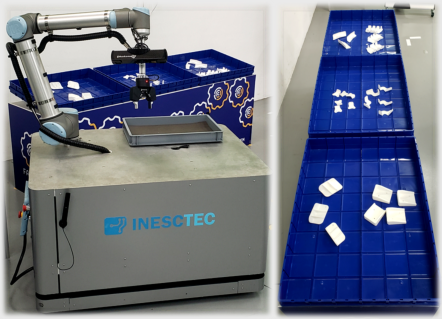
\includegraphics[trim={0cm 0cm 0cm 0cm},clip,width=1\linewidth,angle=0]{Cap5/Figuras/omni_robot_and_bins.pdf}}
\end{tcolorbox}
\caption{(left) Omnidirectional mobile manipulator. (right) Example of objects placed on a bin.}
\label{fig:omni}
}%end resize box
\end{figure}


 \begin{figure}[h!]
 \resizebox{.8\textwidth}{!}{%
 \begin{tcolorbox}
      \centering
      \begin{subfigure}[c]{.23\textwidth}
          \centering
          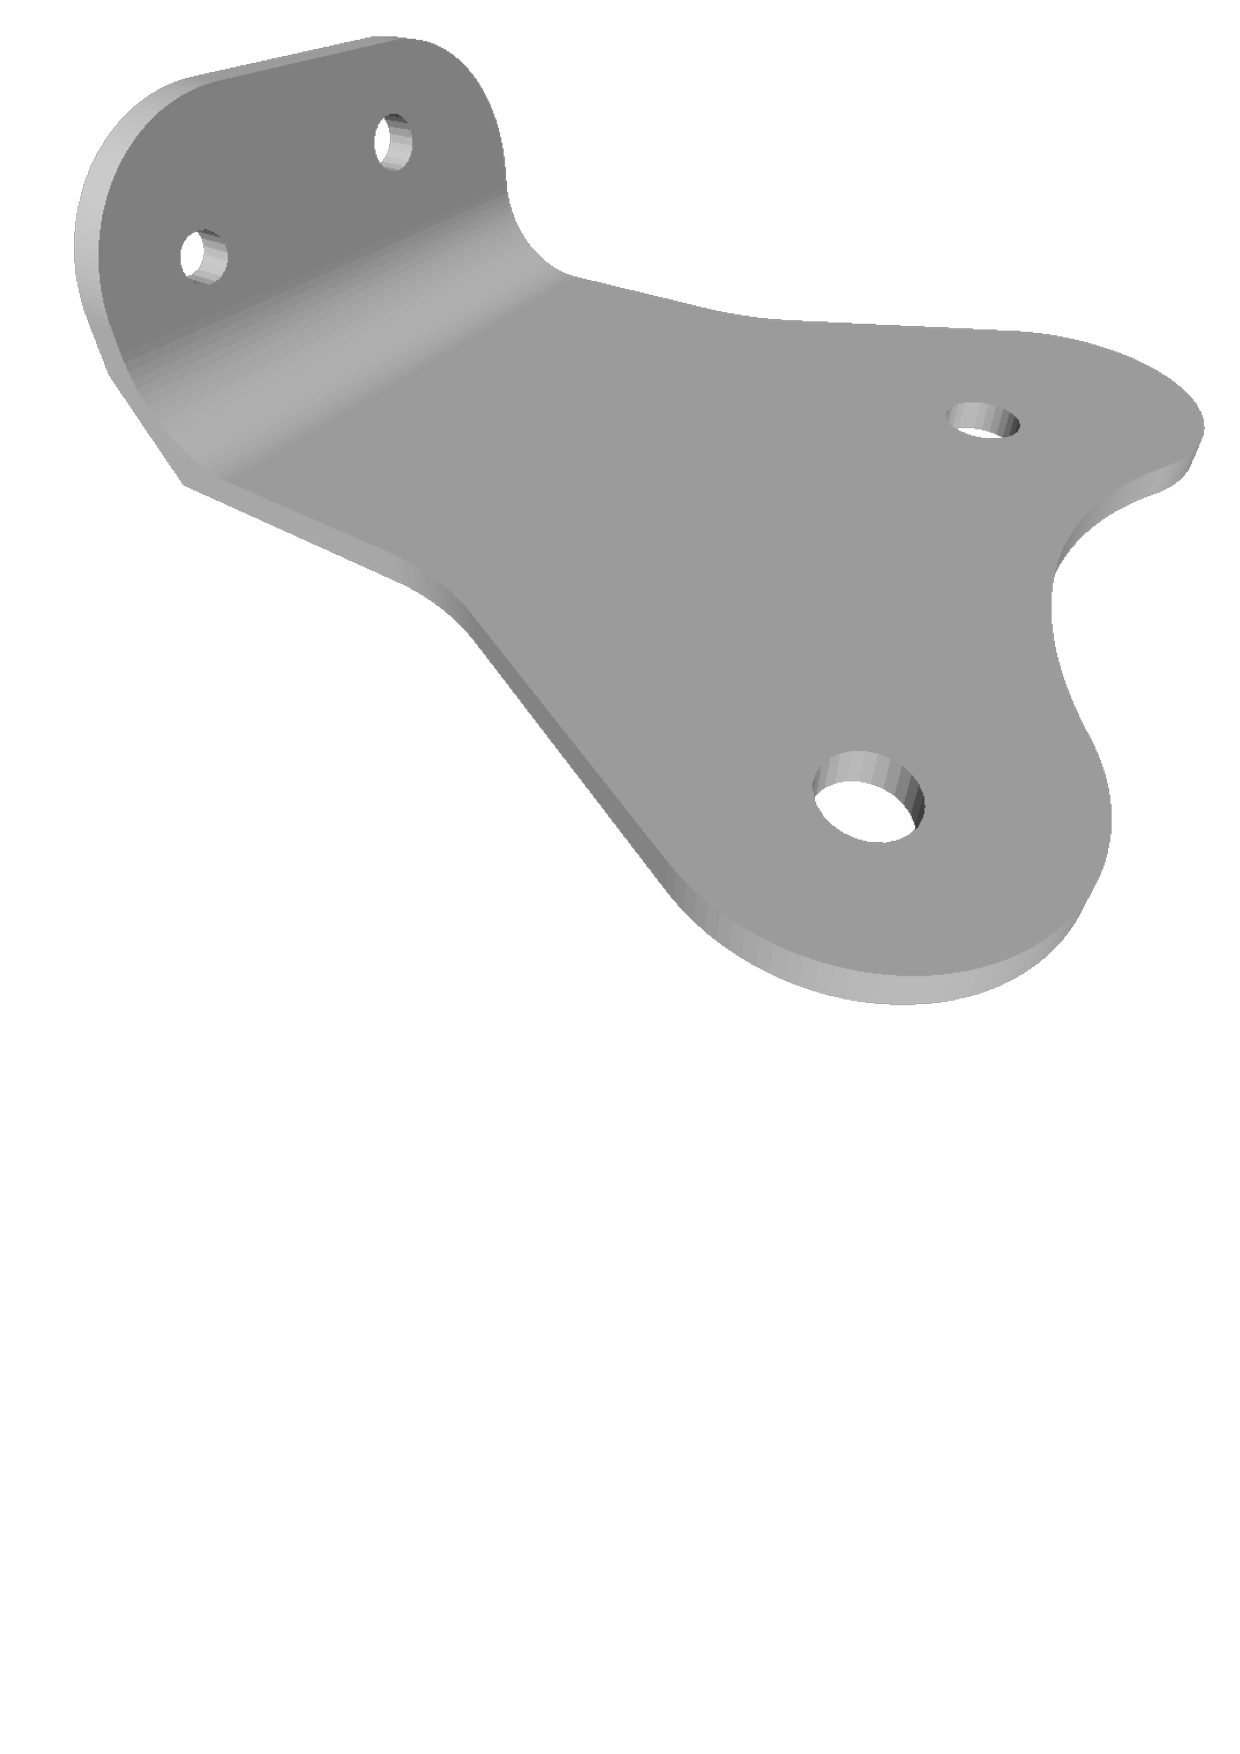
\includegraphics[trim={0cm 12cm 0cm .5cm},clip,width=1\linewidth,angle=0]{Cap5/Figuras/objects/bracket.pdf}
          \caption{}
          \label{fig:bracket}
      \end{subfigure}
      \hfill
      \begin{subfigure}[c]{.23\textwidth}
          \centering
          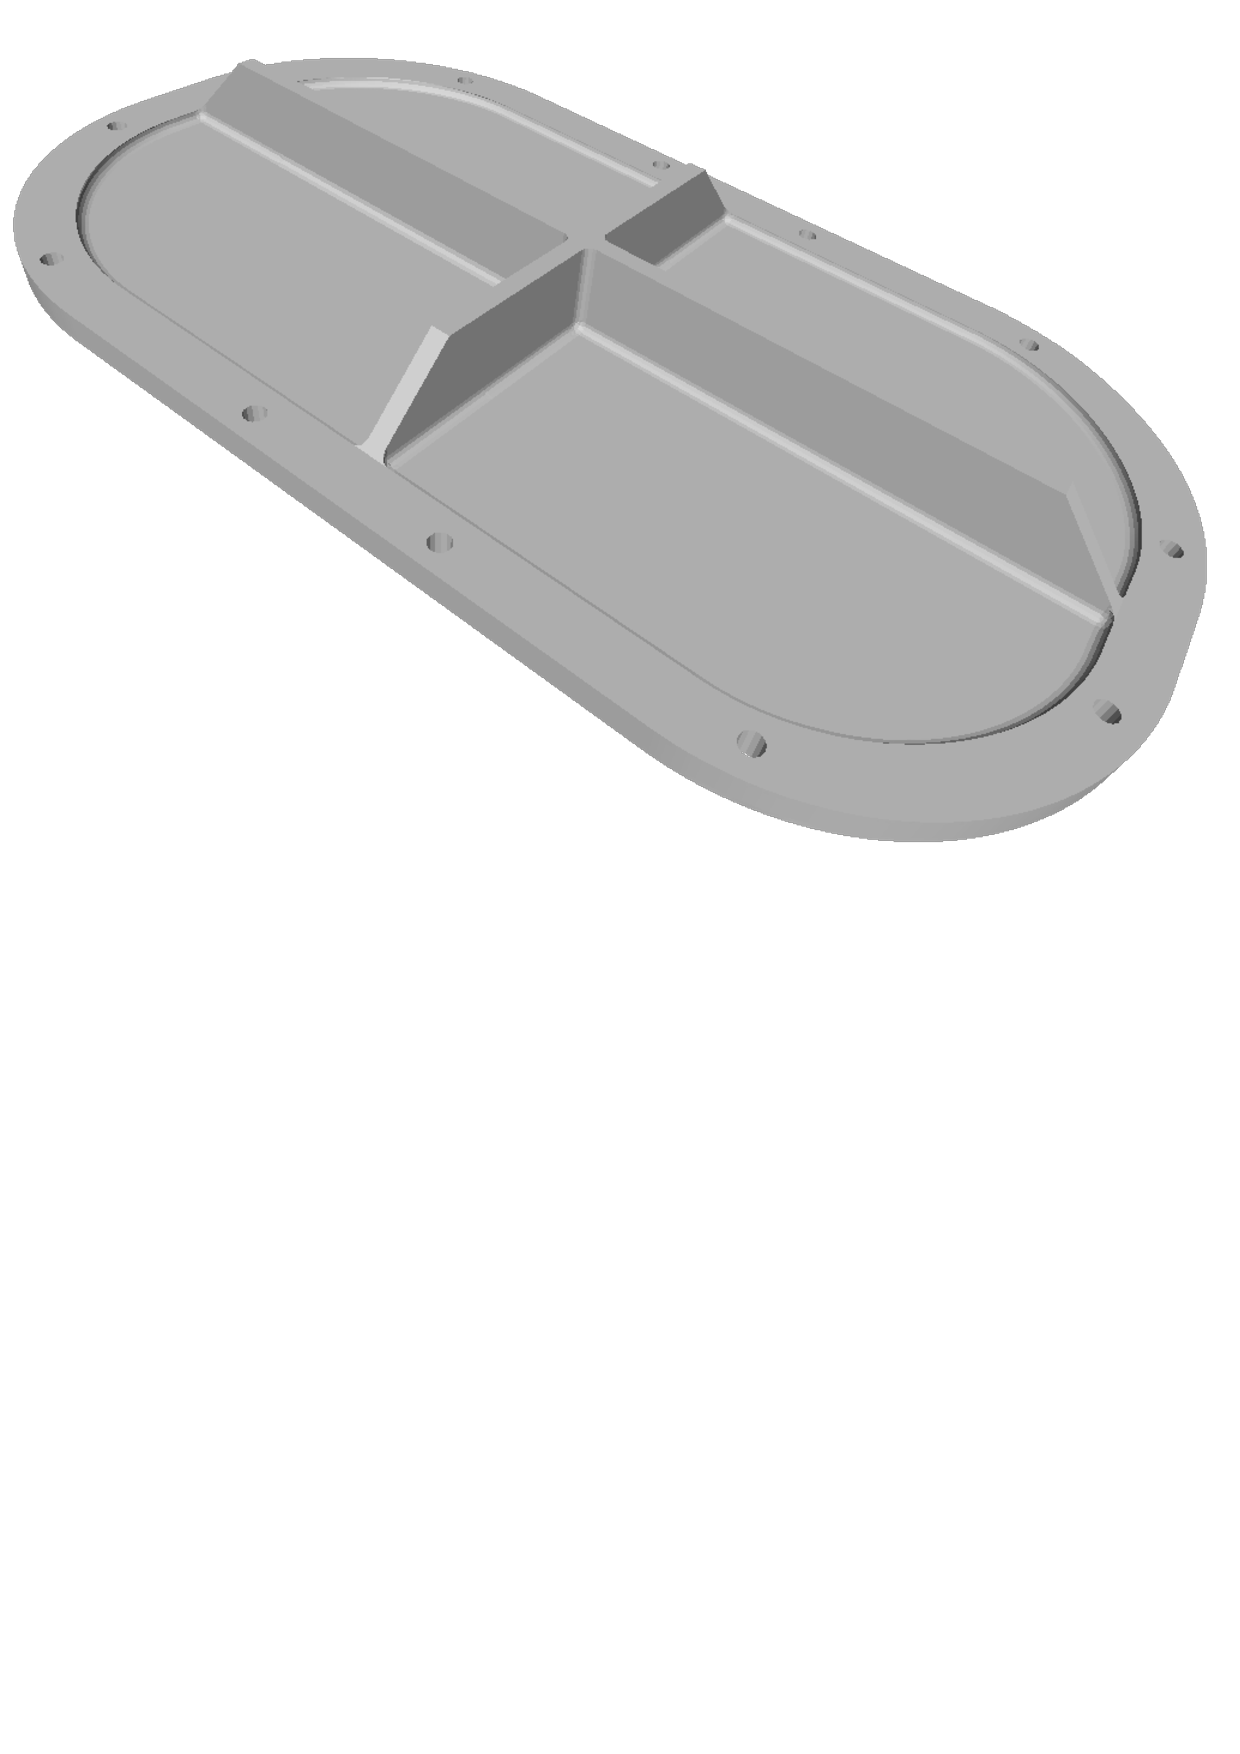
\includegraphics[trim={0cm 12cm 0cm 0cm},clip,width=1\linewidth,angle=0]{Cap5/Figuras/objects/cover_plate.pdf}
          \caption{}
          \label{fig:cover_plate}
      \end{subfigure}
      \hfill
      \begin{subfigure}[c]{.23\textwidth}
          \centering
          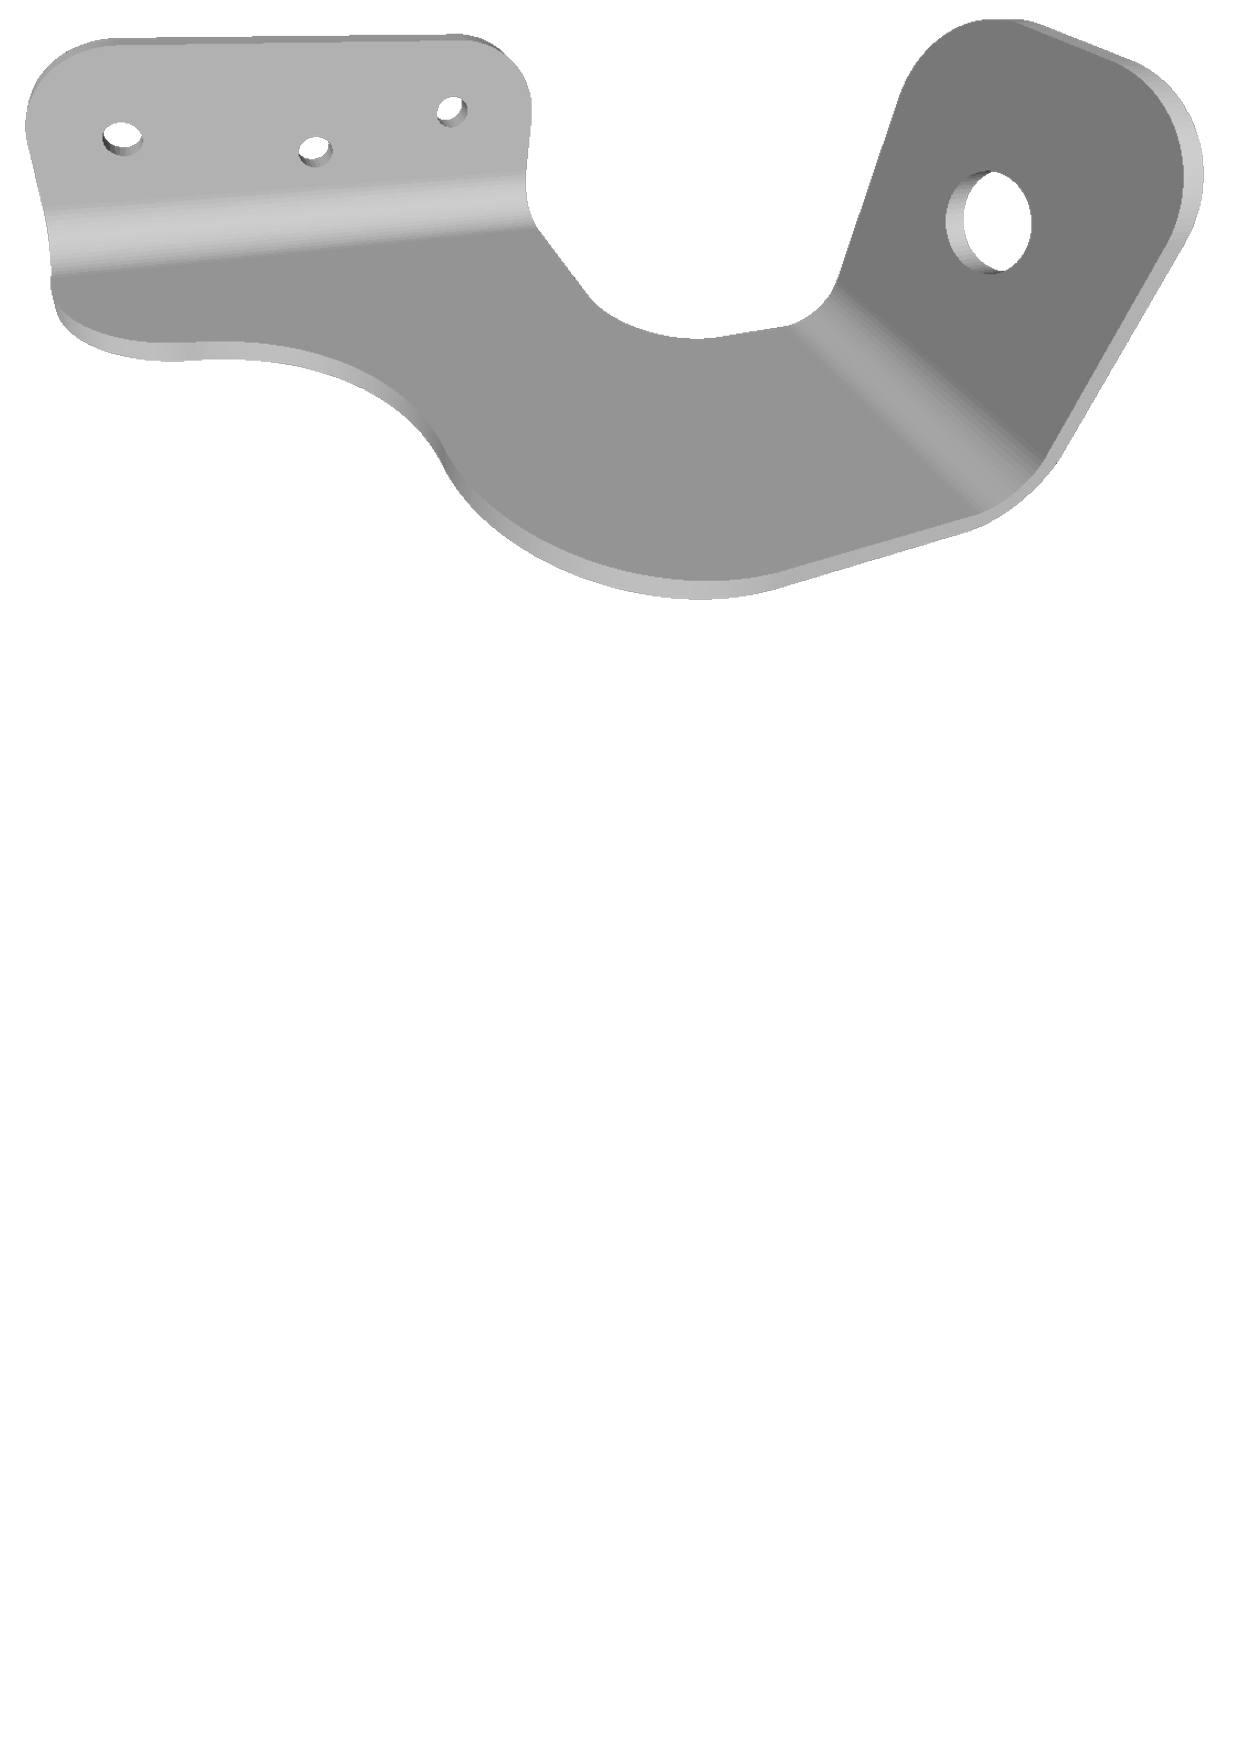
\includegraphics[trim={0cm 17cm 0cm 0cm},clip,width=1\linewidth,angle=0]{Cap5/Figuras/objects/double_side_bracket.pdf}
          \caption{}
          \label{fig:Double_side_bracket}
      \end{subfigure}
      \hfill
      \begin{subfigure}[c]{.23\textwidth}
         \centering
         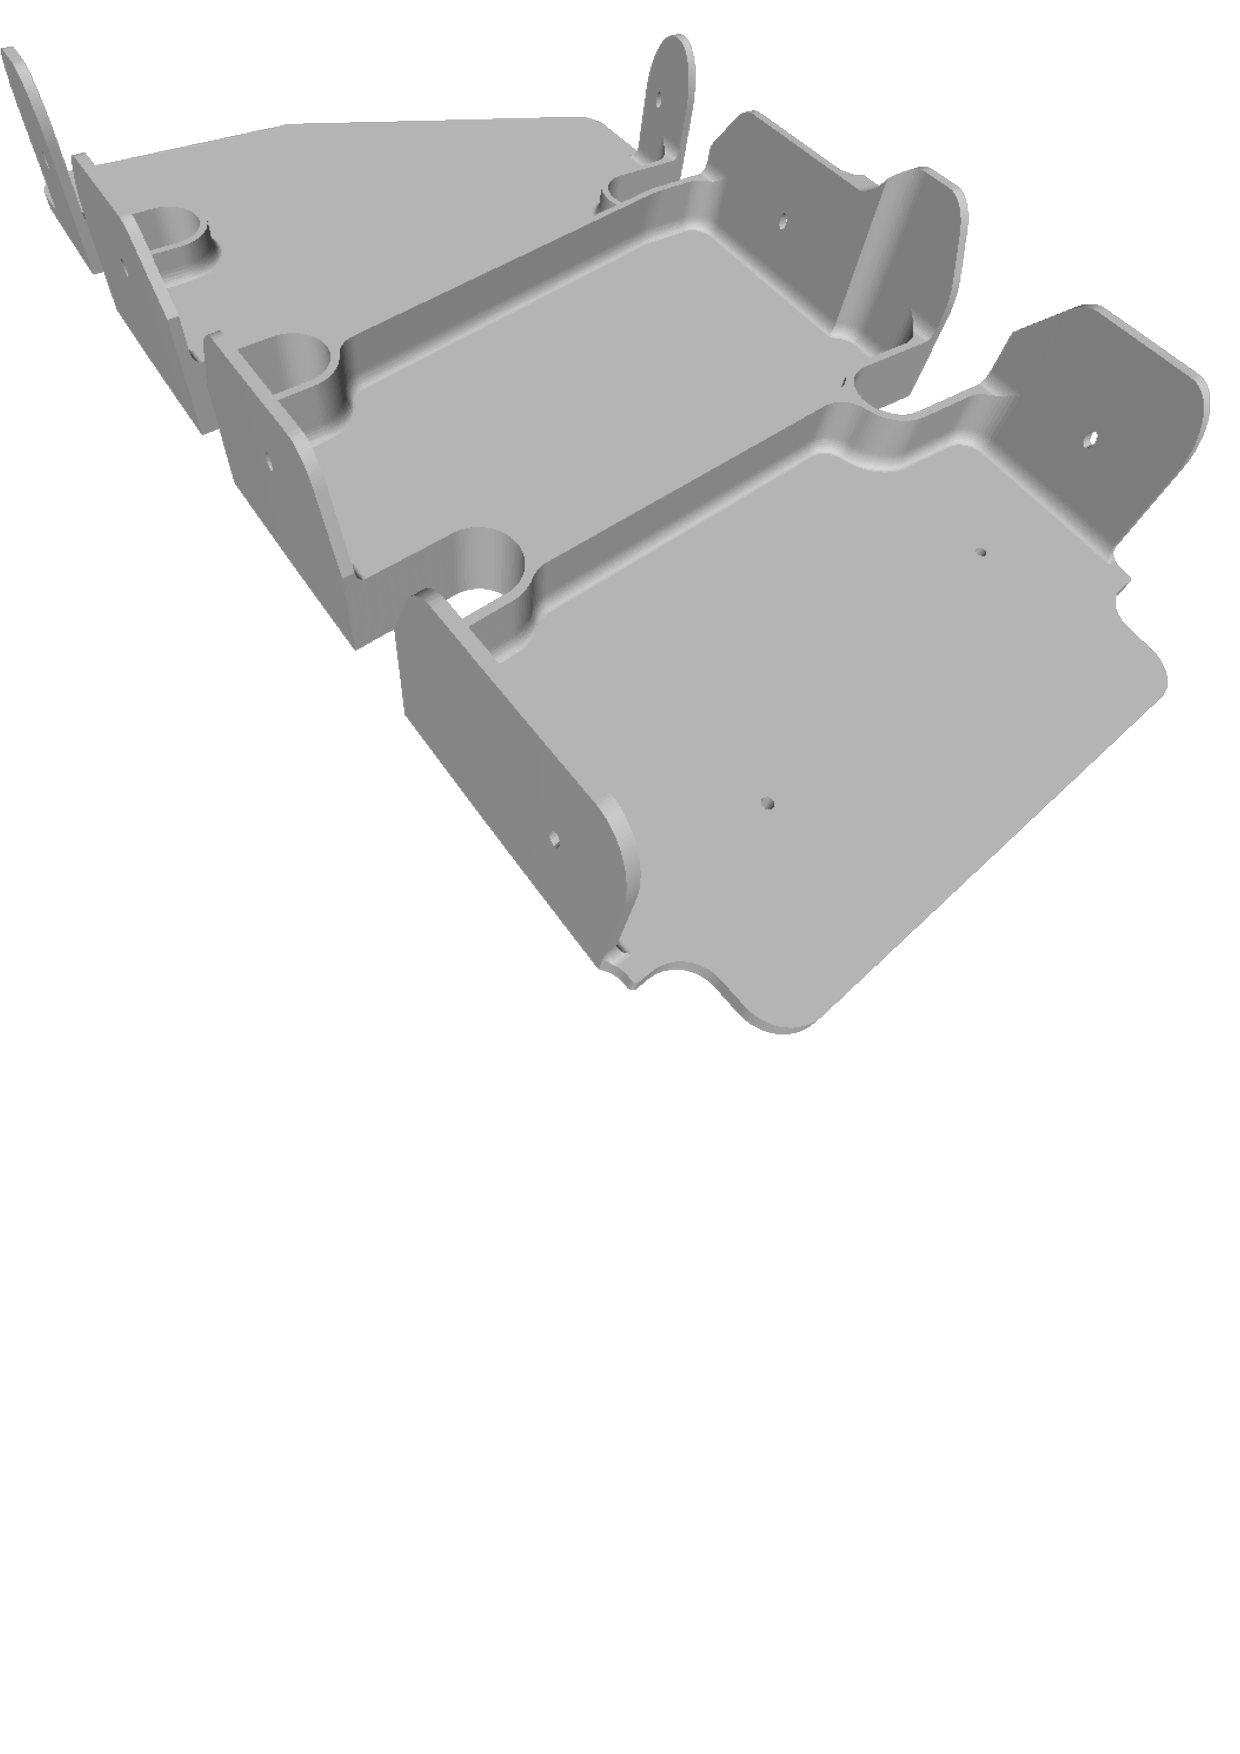
\includegraphics[trim={0cm 9cm 0cm 0cm},clip,width=1\linewidth,angle=0]{Cap5/Figuras/objects/multi_side_bracket.pdf}
         \caption{}
         \label{fig:multi_side_bracket}
      \end{subfigure}
      \hfill
      \begin{subfigure}[c]{.23\textwidth}
         \centering
         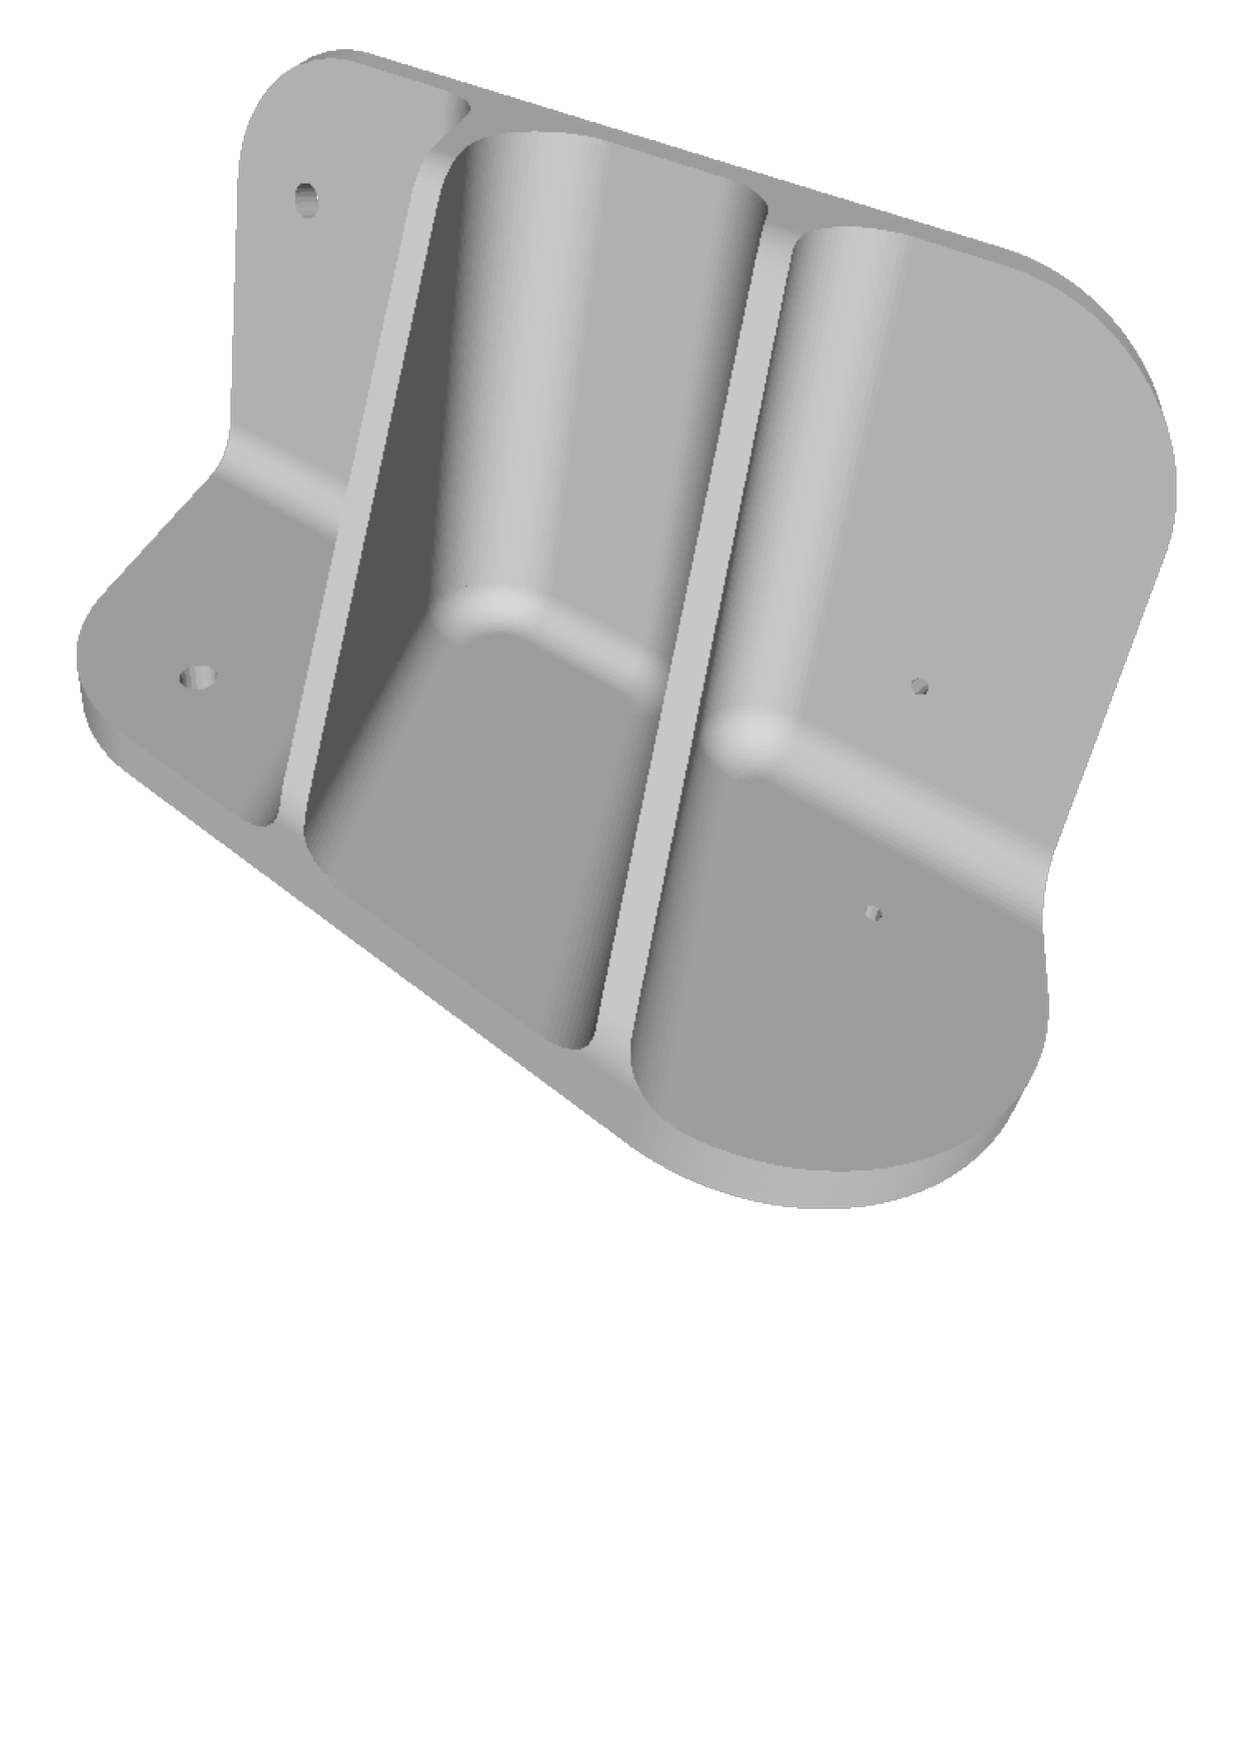
\includegraphics[trim={0cm 9cm 0cm 0cm},clip,width=1\linewidth,angle=0]{Cap5/Figuras/objects/reinforced_bracket.pdf}
         \caption{}
         \label{fig:reinforced_bracket}
      \end{subfigure}
      \hfill
      \begin{subfigure}[c]{.23\textwidth}
         \centering
         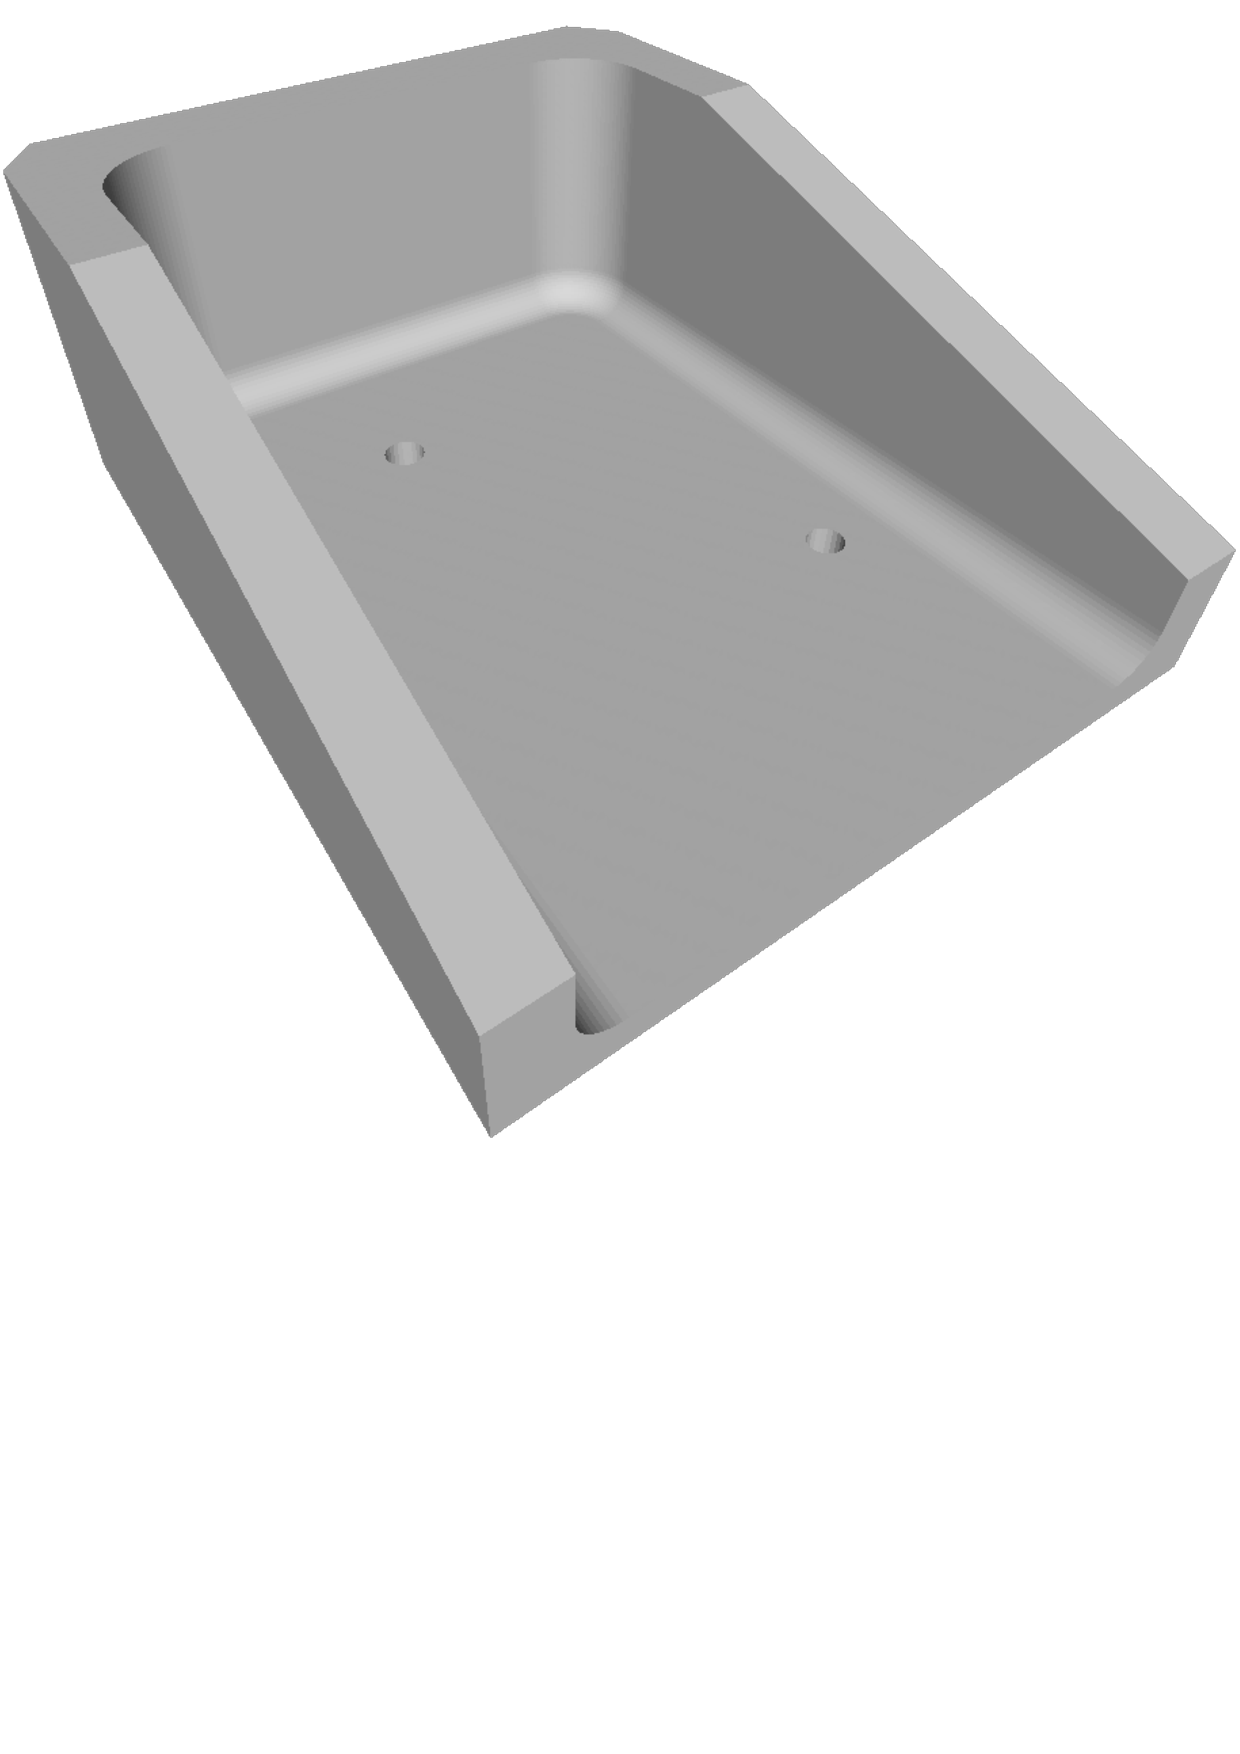
\includegraphics[trim={0cm 9cm 0cm 0cm},clip,width=1\linewidth,angle=0]{Cap5/Figuras/objects/single_side_bracket.pdf}
         \caption{}
         \label{fig:single_side_bracket}
      \end{subfigure}
      \hfill
      \begin{subfigure}[c]{.23\textwidth}
         \centering
         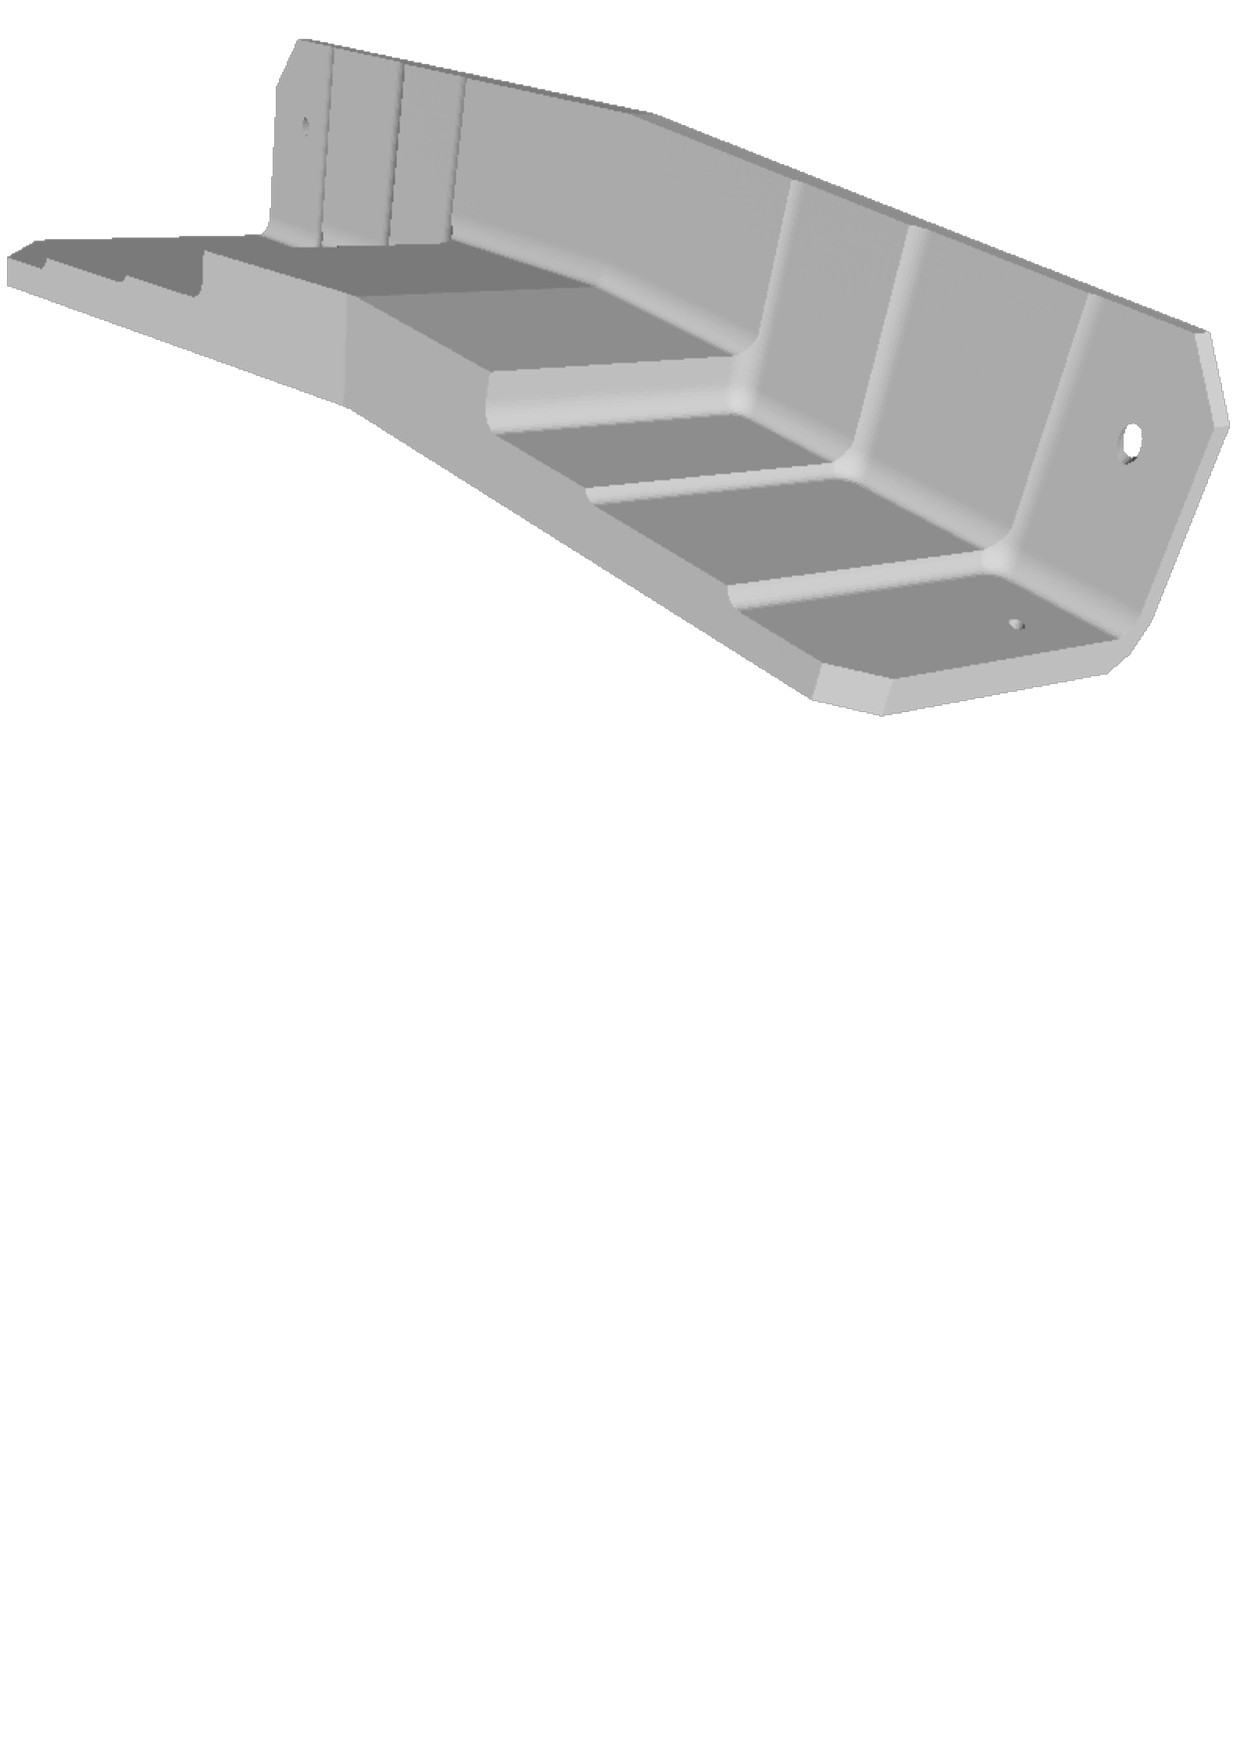
\includegraphics[trim={0cm 17cm 0cm 0cm},clip,width=1\linewidth,angle=0]{Cap5/Figuras/objects/support_bracket.pdf}
         \caption{}
         \label{fig:support_bracket}
      \end{subfigure}
      \hfill
      \begin{subfigure}[c]{.23\textwidth}
         \centering
         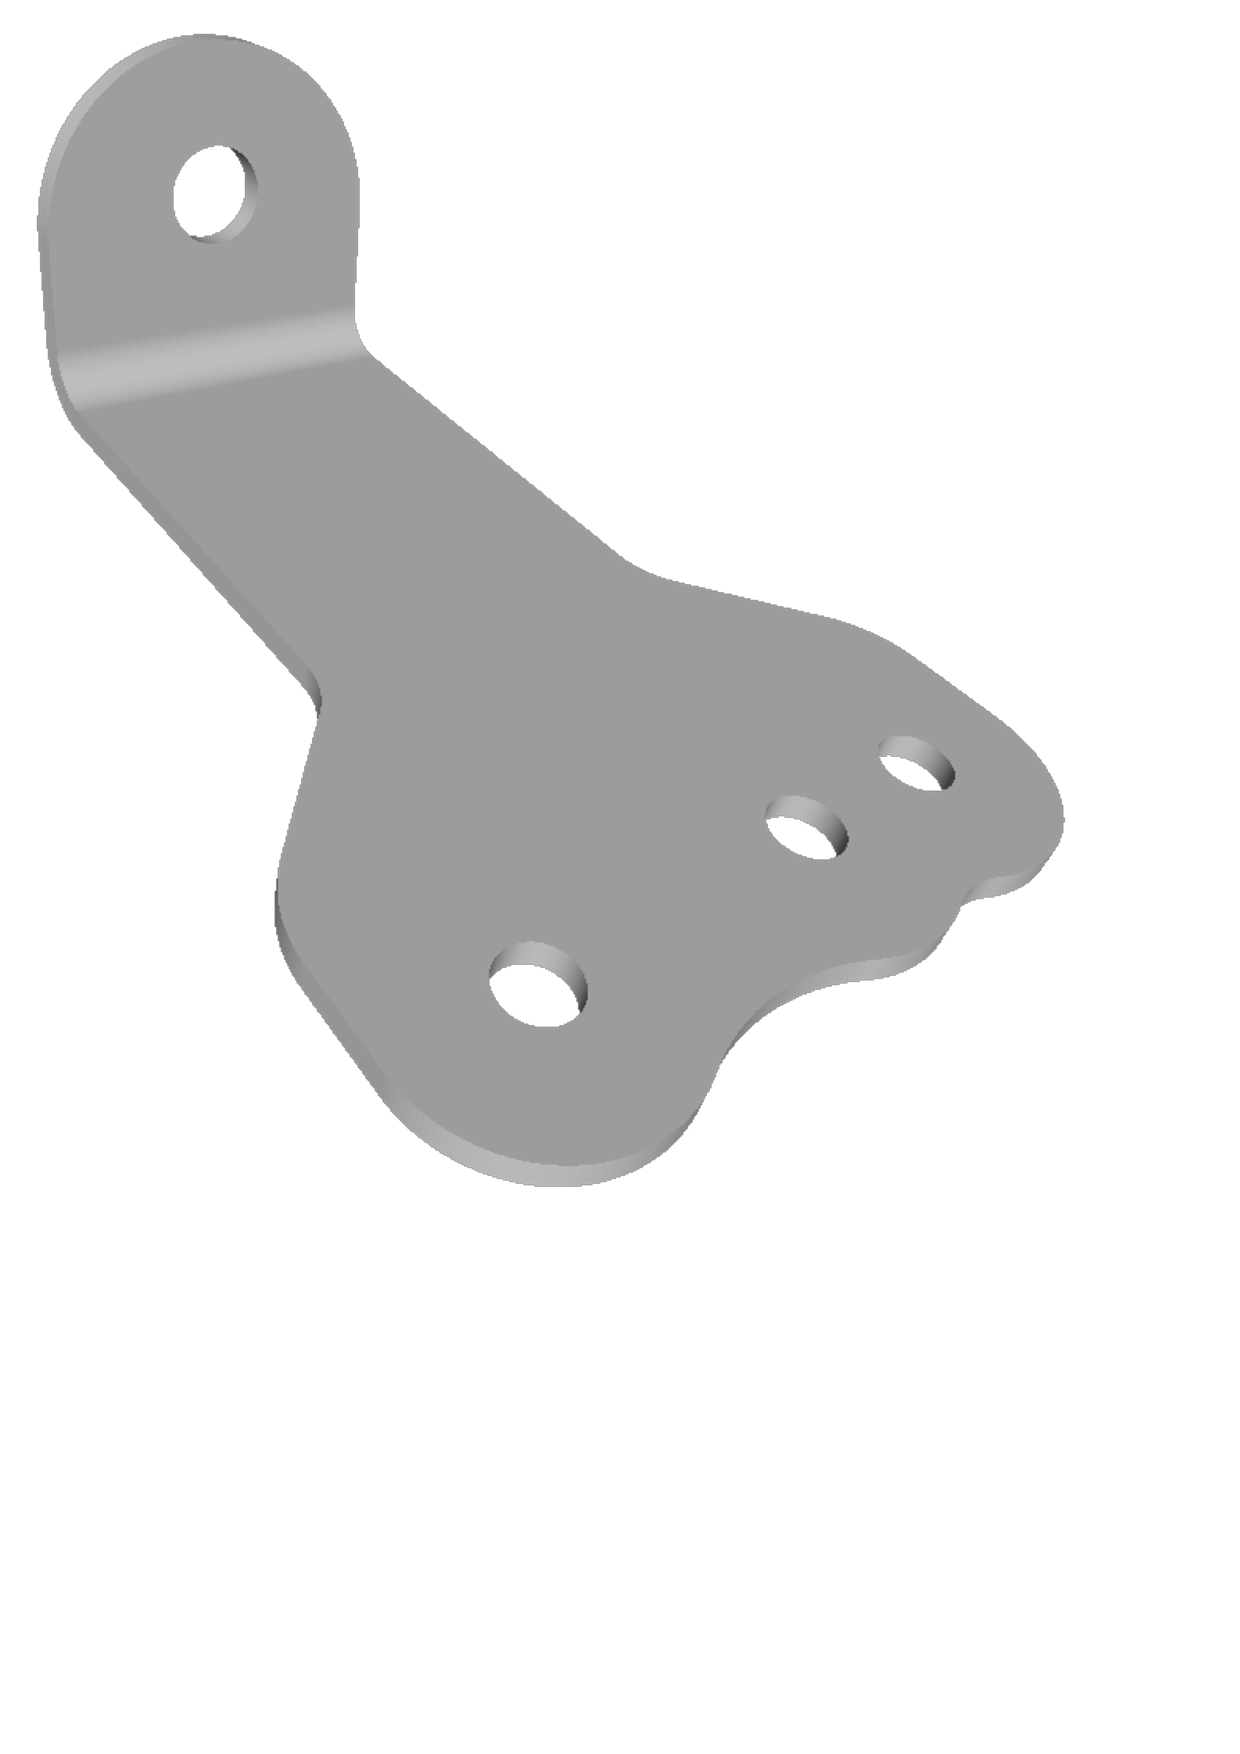
\includegraphics[trim={0cm 8cm 0cm 0cm},clip,width=1\linewidth,angle=0]{Cap5/Figuras/objects/t_bracket.pdf}
         \caption{}
         \label{fig:t_bracket}
      \end{subfigure}
     \end{tcolorbox}
     \caption{Objects from FASTEN setup. (a) Bracket (b) Cover plate (c) Double side bracket (d) Multi side bracket (e) Reinforced bracket (f) Single side bracket (g) Support bracket (h) T-bracket.}
     \label{fig:obj_fasten}
   }%end of resize box      
 \end{figure}

The same robot configuration is used for the Mari4Yard and the Produtech 4S\&C, but with one major difference: a larger gripper is used, the RobotiQ 2F-140~\cite{robotiq_grippers}. The maximum opening of the adaptive fingers of 140 millimetres makes it possible to grasp larger objects, which is the case with the set of marine objects provided by \cred{TODO}. The JPM~\cite{jpm} supplied the objects to Produtech 4S\&C, which deals with intralogistics and fast consumer goods. In these cases, the robot is equipped with a computer with an Intel Core i7-6700HQ processor and a 32GB 2133 MHz memory RAM. The objects for Mari4Yard and Produtech 4S\&C are shown in the Figures~\ref{fig:obj_mari4yard} and ~\ref{fig:obj_produtech} respectively.

%These test-case differences allow to test the pipeline modularity and deployment flexibility. The specific pipeline configuration process and achieved results are presented in the following sections.


 \begin{figure}[h!]
 \resizebox{.8\textwidth}{!}{%
 \begin{tcolorbox}
      \centering
      \begin{subfigure}[c]{.45\textwidth}
          \centering
          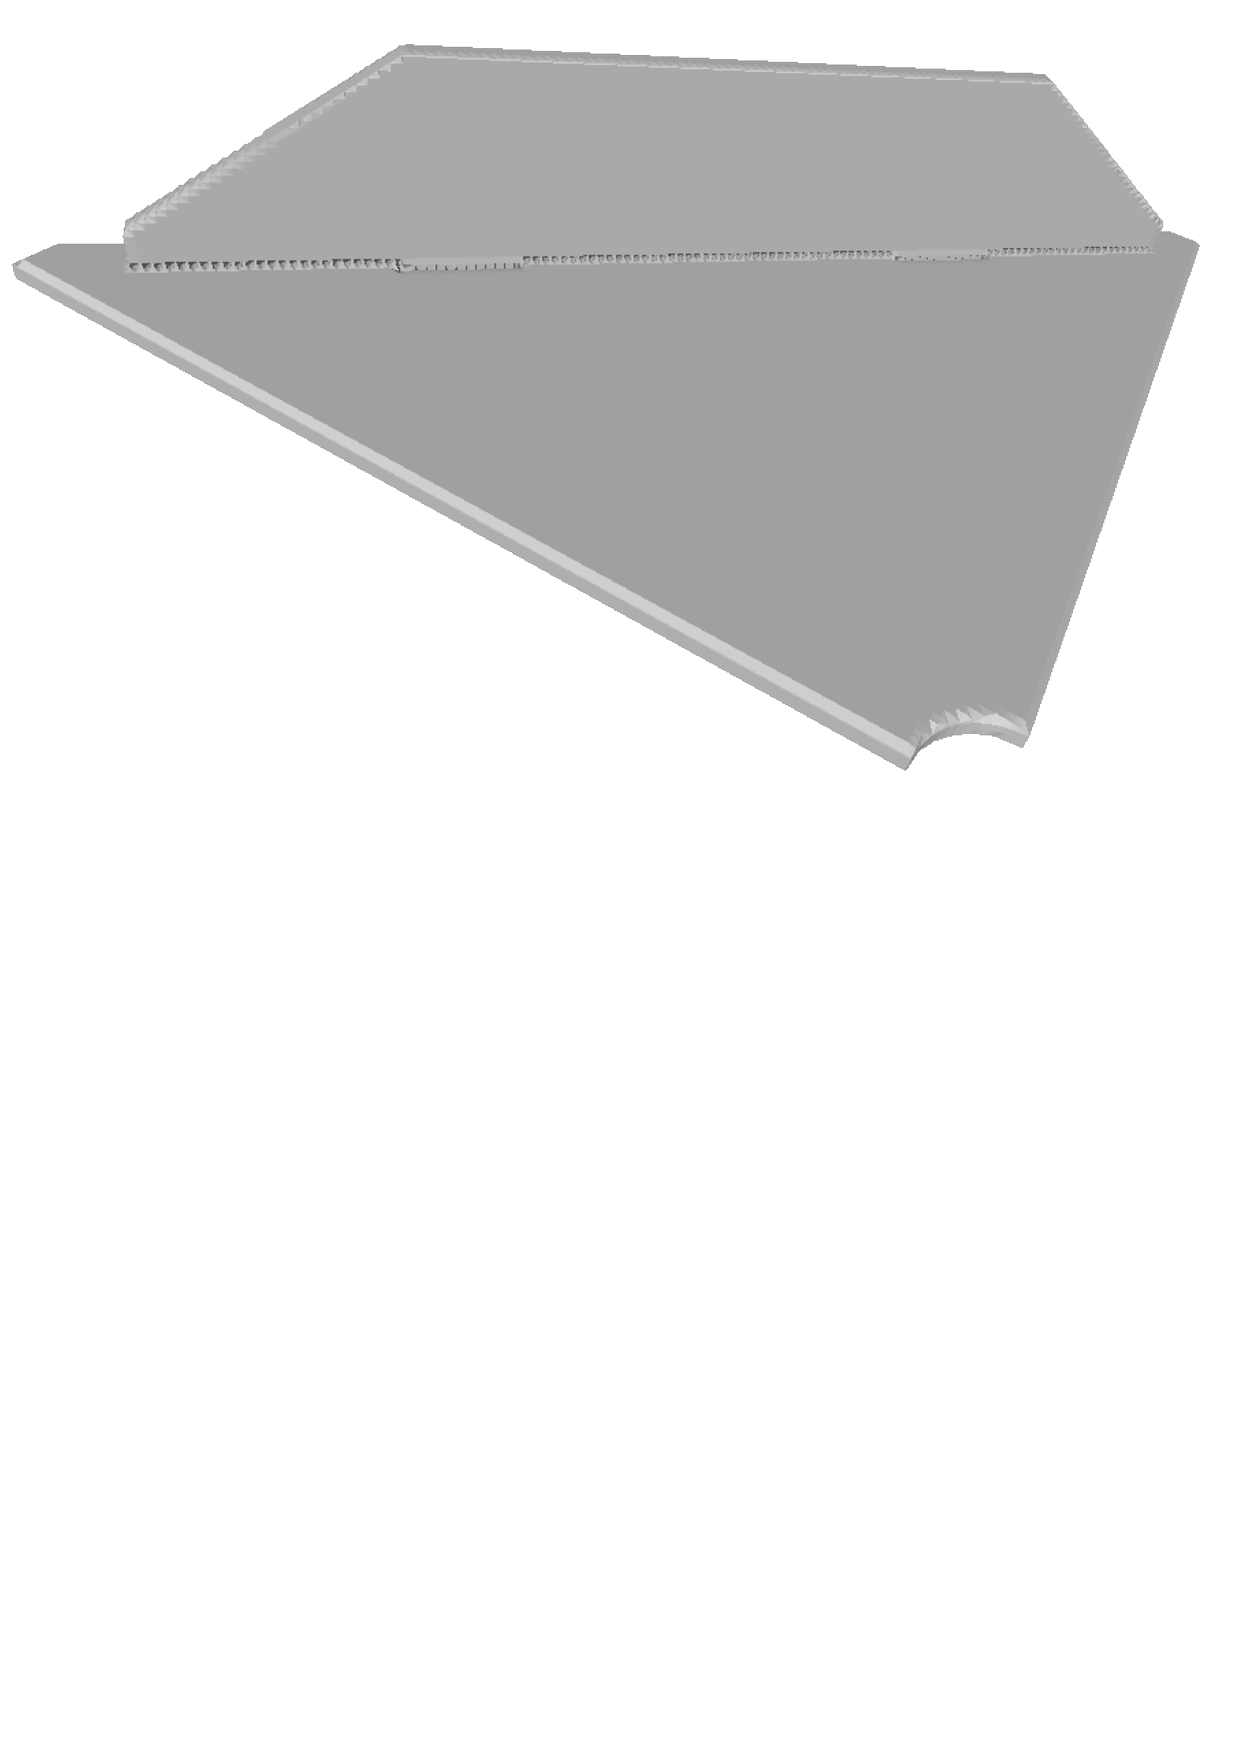
\includegraphics[trim={0cm 16cm 0cm .5cm},clip,width=1\linewidth,angle=0]{Cap5/Figuras/objects/triangle_bracket.pdf}
          \caption{}
          \label{fig:triangle_bracket}
      \end{subfigure}
      \hfill
      \begin{subfigure}[c]{.45\textwidth}
          \centering
          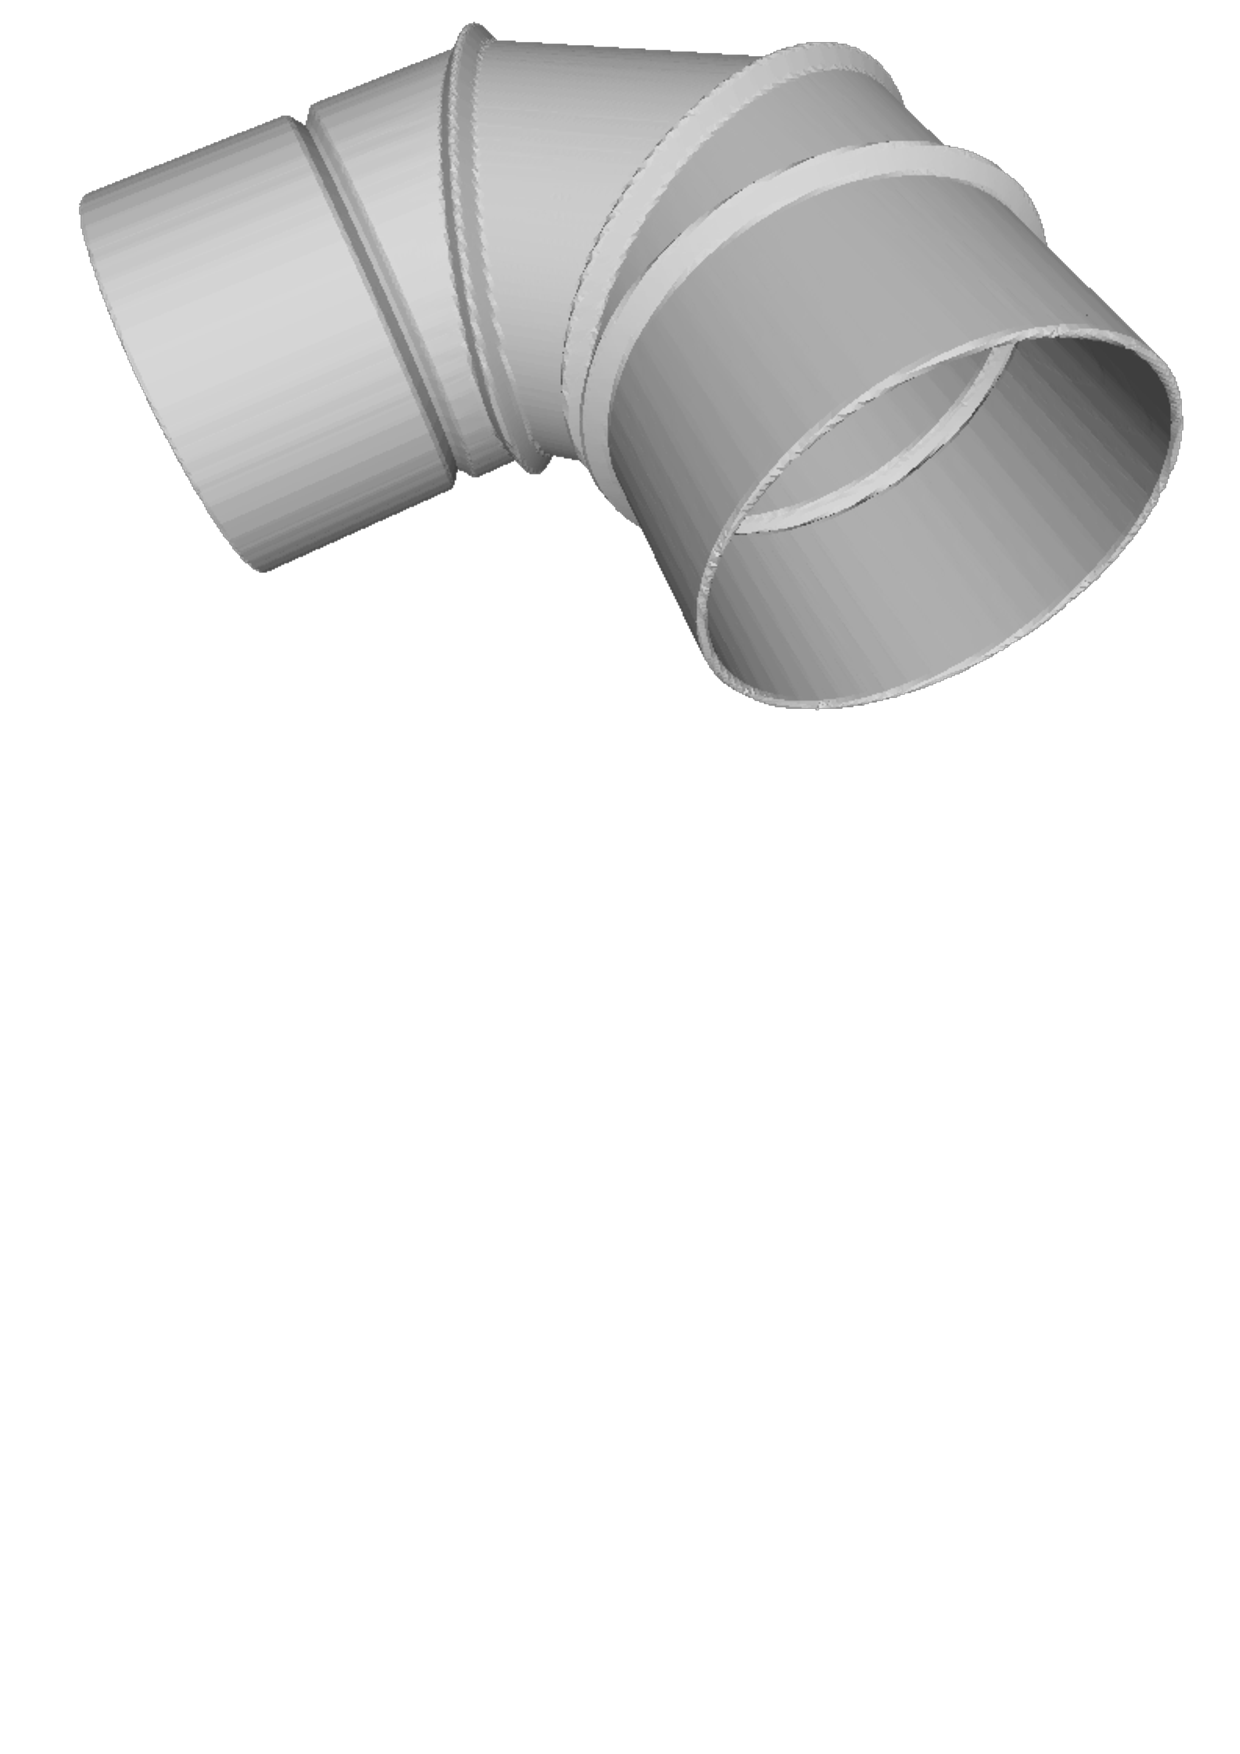
\includegraphics[trim={0cm 16cm 0cm 0cm},clip,width=1\linewidth,angle=0]{Cap5/Figuras/objects/90_elbow_flue_pipe.pdf}
          \caption{}
          \label{fig:90_elbow_flue_pipe}
      \end{subfigure}
     \end{tcolorbox}
     \caption{Objects from MARI4YARD use case. (a) Triangle bracket (b) 90º elbow flue pipe.}
     \label{fig:obj_mari4yard}
   }%end of resize box      
 \end{figure}

 \begin{figure}[h!]
 \resizebox{.75\textwidth}{!}{%
 \begin{tcolorbox}
      \centering
      \begin{subfigure}[c]{.32\textwidth}
          \centering
          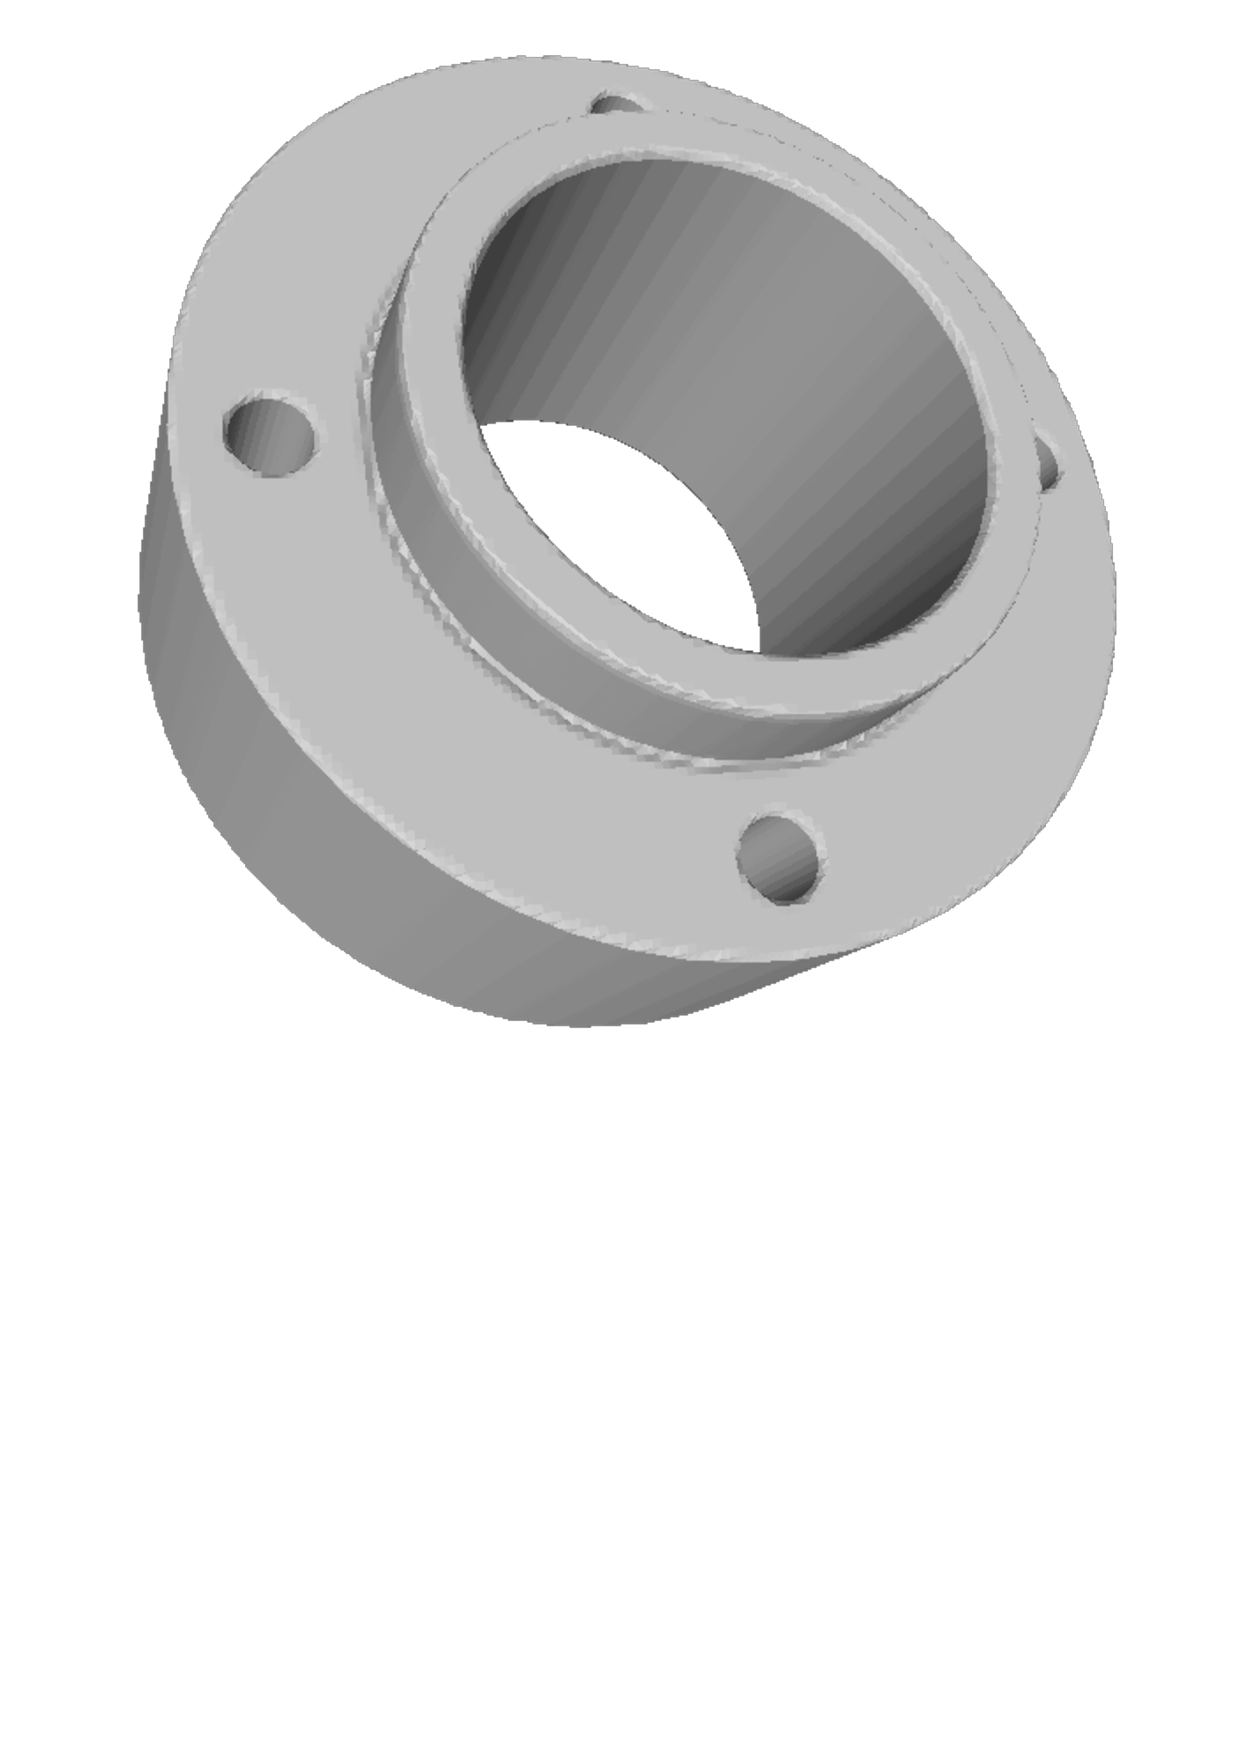
\includegraphics[trim={0cm 12cm 0cm .5cm},clip,width=1\linewidth,angle=0]{Cap5/Figuras/objects/falange_piece.pdf}
          \caption{}
          \label{fig:falange_piece}
      \end{subfigure}
      \hfill
      \begin{subfigure}[c]{.32\textwidth}
          \centering
          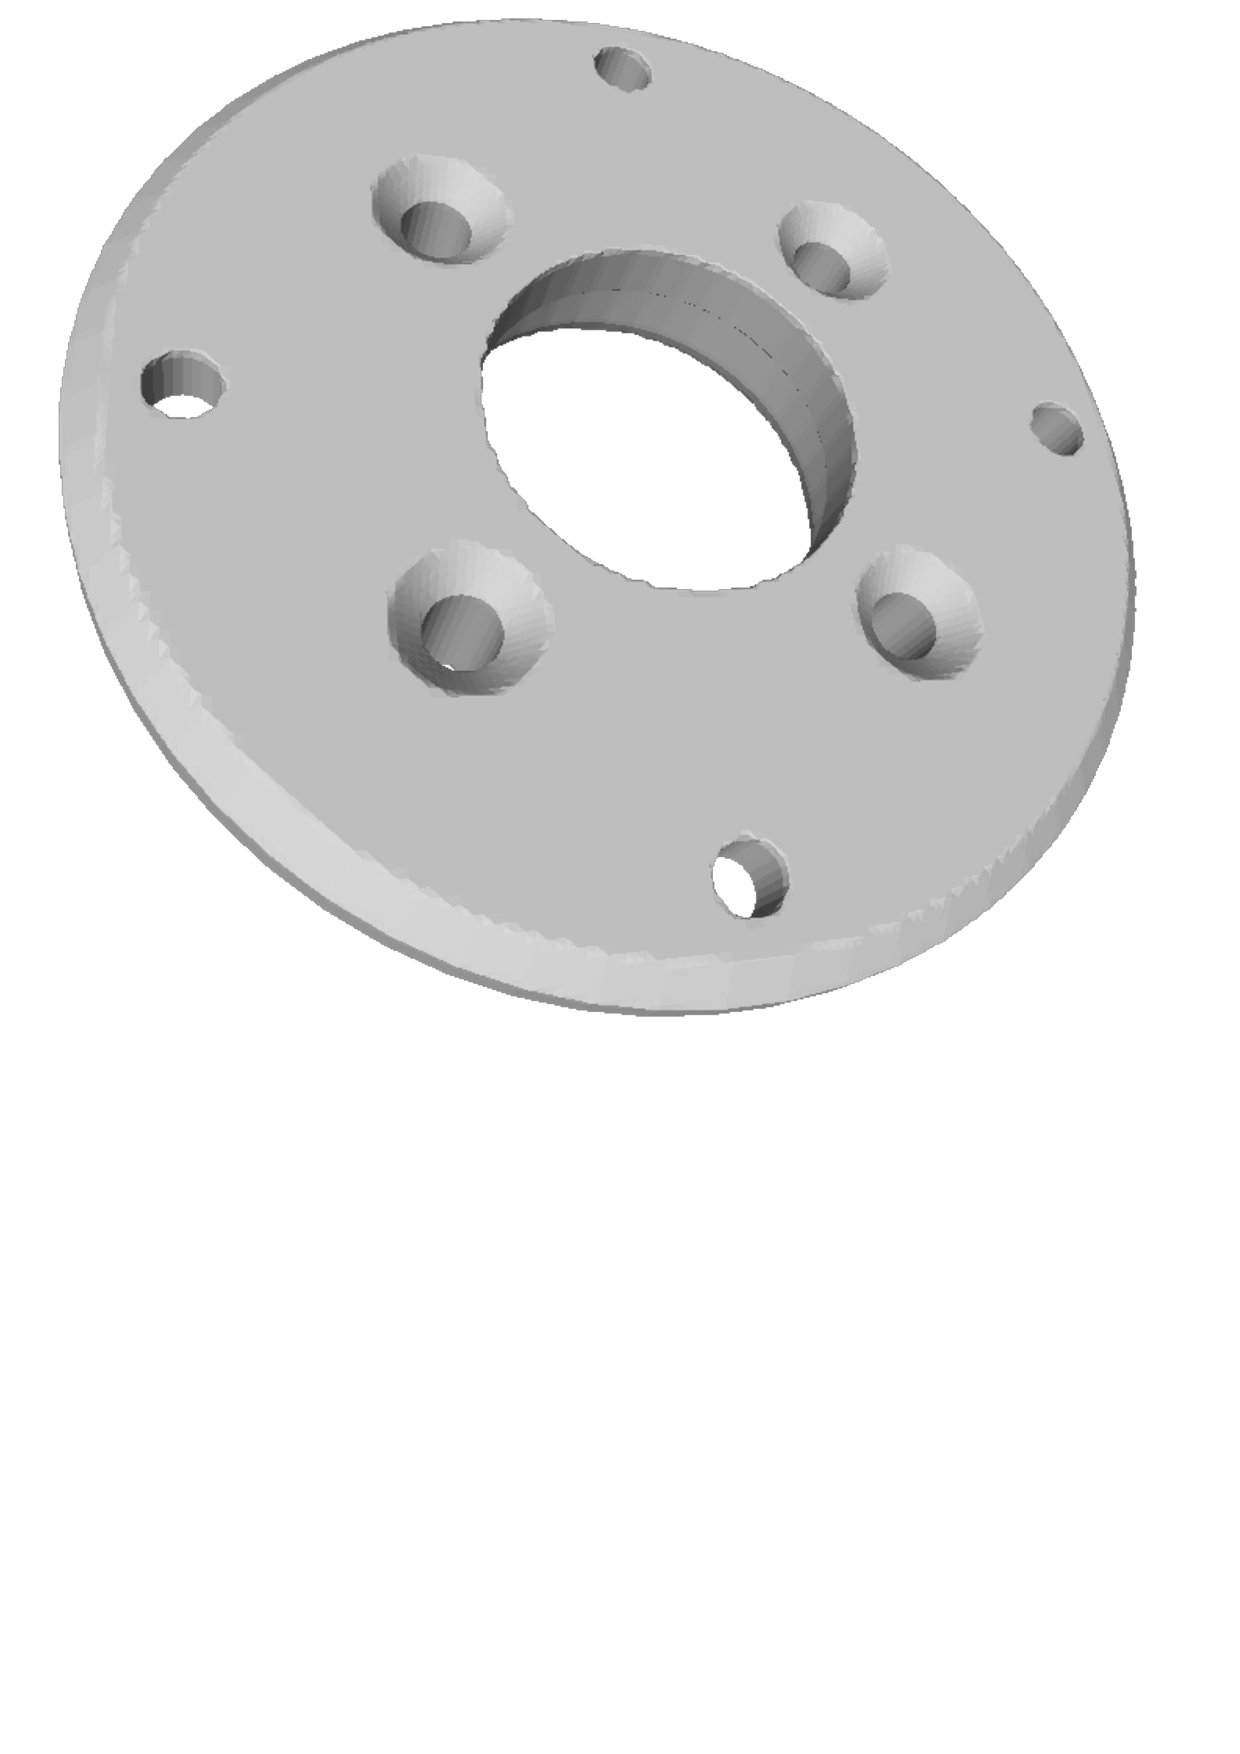
\includegraphics[trim={0cm 12cm 0cm 0cm},clip,width=1\linewidth,angle=0]{Cap5/Figuras/objects/bearing_holder.pdf}
          \caption{}
          \label{fig:bearing_holder}
      \end{subfigure}
      \hfill
      \begin{subfigure}[c]{.32\textwidth}
          \centering
          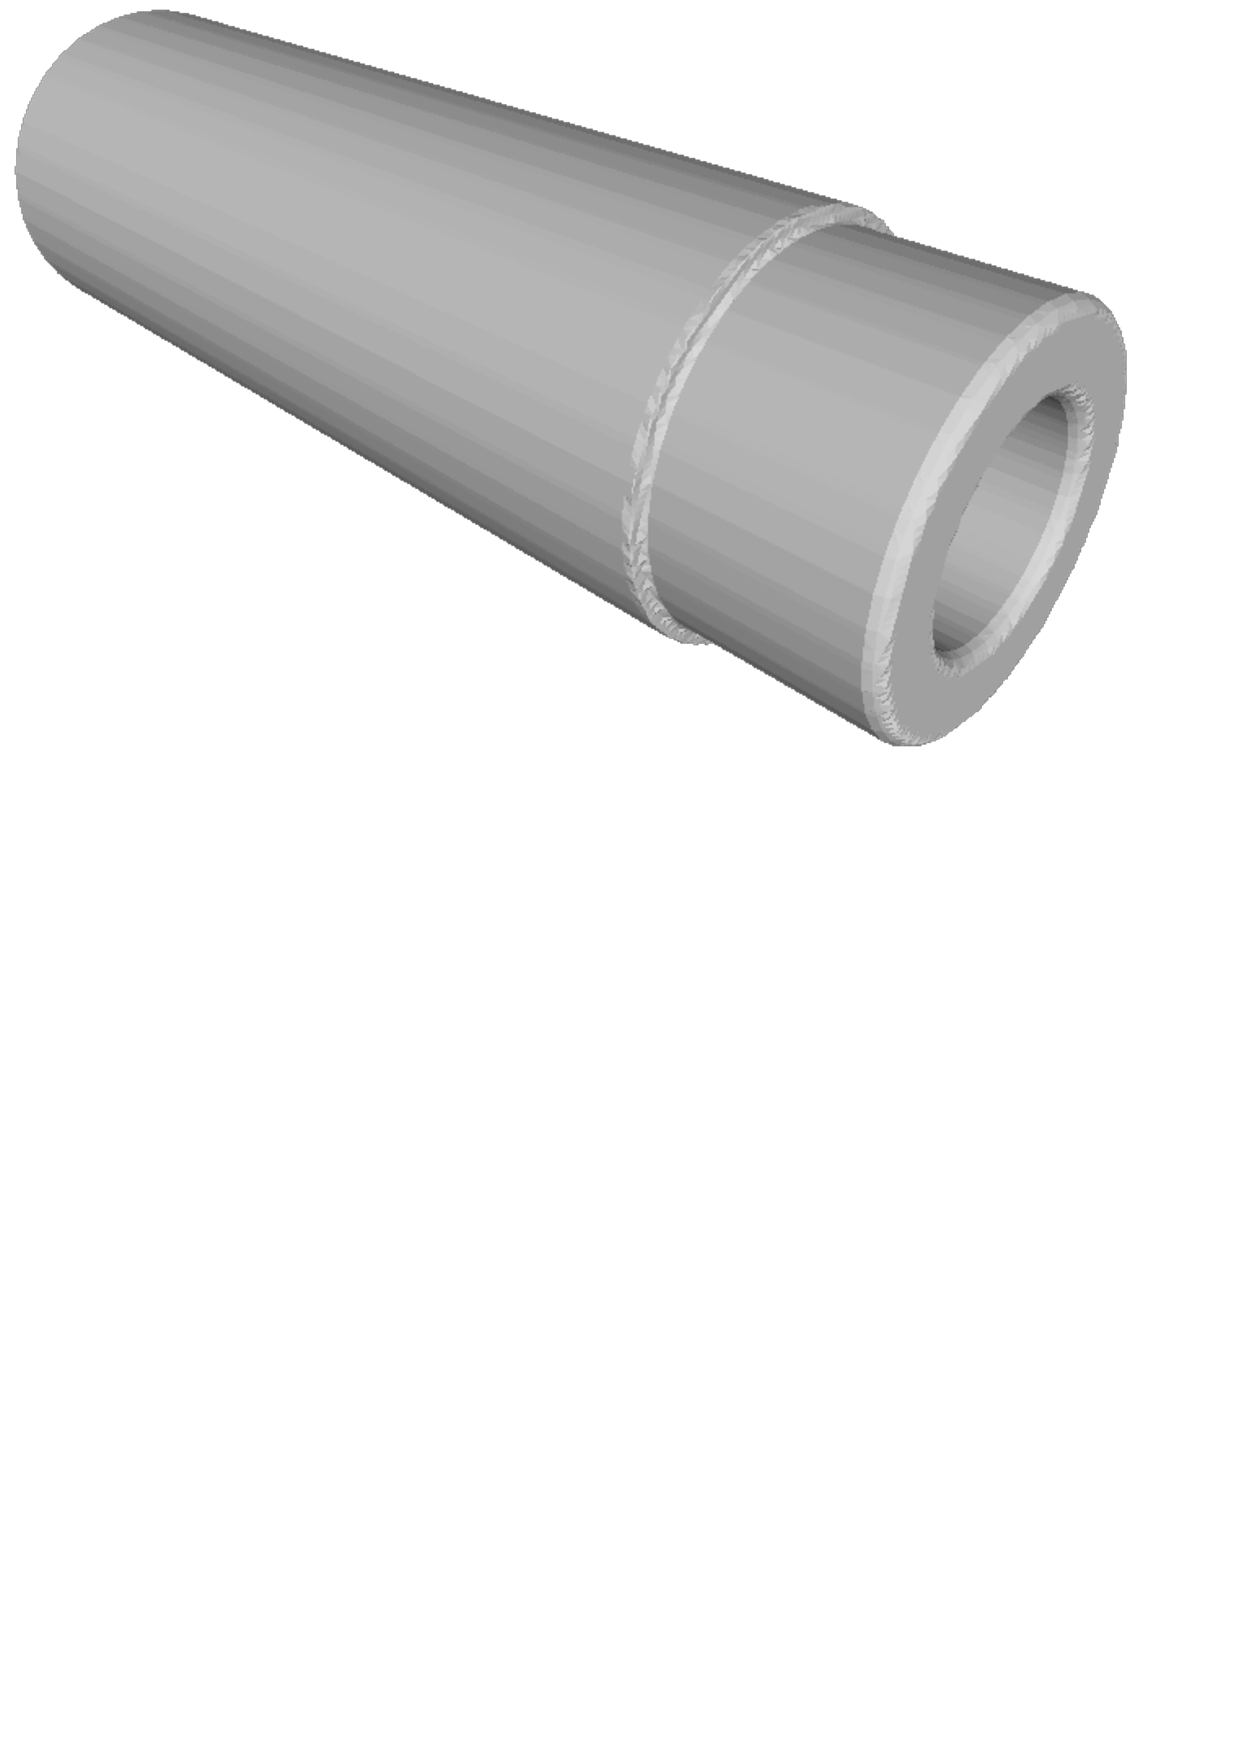
\includegraphics[trim={0cm 17cm 0cm 0cm},clip,width=1\linewidth,angle=0]{Cap5/Figuras/objects/rod.pdf}
          \caption{}
          \label{fig:rod}
      \end{subfigure}
     \end{tcolorbox}
     \caption{Objects from PRODUTECH 4S\&C use case. (a) Falange piece (b) Bearing holder (c) Rod.}
     \label{fig:obj_produtech}
   }%end of resize box      
 \end{figure}


\section{Grasping Architecture Evaluation}
\label{cap5:grasping_planner_evaluation}


Once the grippers are defined in all projects, their 3D model is represented in Figure~\ref{fig:gripper_models}: the left one is used to test and visualise the possible grasping solutions, while the second one is effectively used in the optimisation step. Both models are modelled with joint movement capabilities. However, only the second model considers the contact model, i.e. the interaction of the physical model with the visual model. Consequently, the model used in the optimisation is simplified and reduces the computational complexity and possible collisions between the links of the gripper itself.

\begin{figure}[h!]
\resizebox{.7\textwidth}{!}{%
\begin{tcolorbox}
\centerline{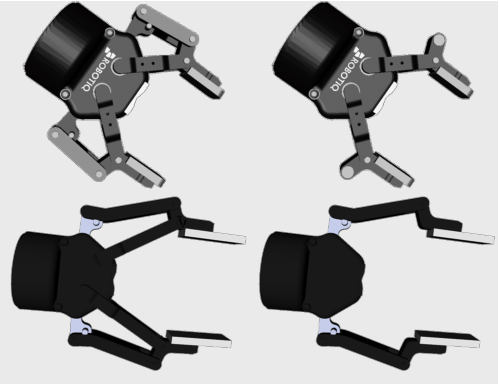
\includegraphics[trim={0cm 0cm 0cm 0cm},clip,width=1\linewidth,angle=0]{Cap5/Figuras/2f_models.pdf}}
\end{tcolorbox}
\caption{Gripper 3D models used. Complete model (left) and simplified model (right).}
\label{fig:gripper_models}
}%end resize box
\end{figure}

% TODO: Continuar correção textual daquin este capitulo

An arbitrary number of contact points are selected for the contact model, these points constitute the \ac{ICR}, and they belong to the fingertips (Figure~\ref{fig:icr}). The considered number of points in the \ac{ICR} affects the algorithm performance, i.e., a large set of points increases the grasping reliability but could compromises the algorithm convergence.

\begin{figure}[h!]
\resizebox{.8\textwidth}{!}{%
\begin{tcolorbox}
\centerline{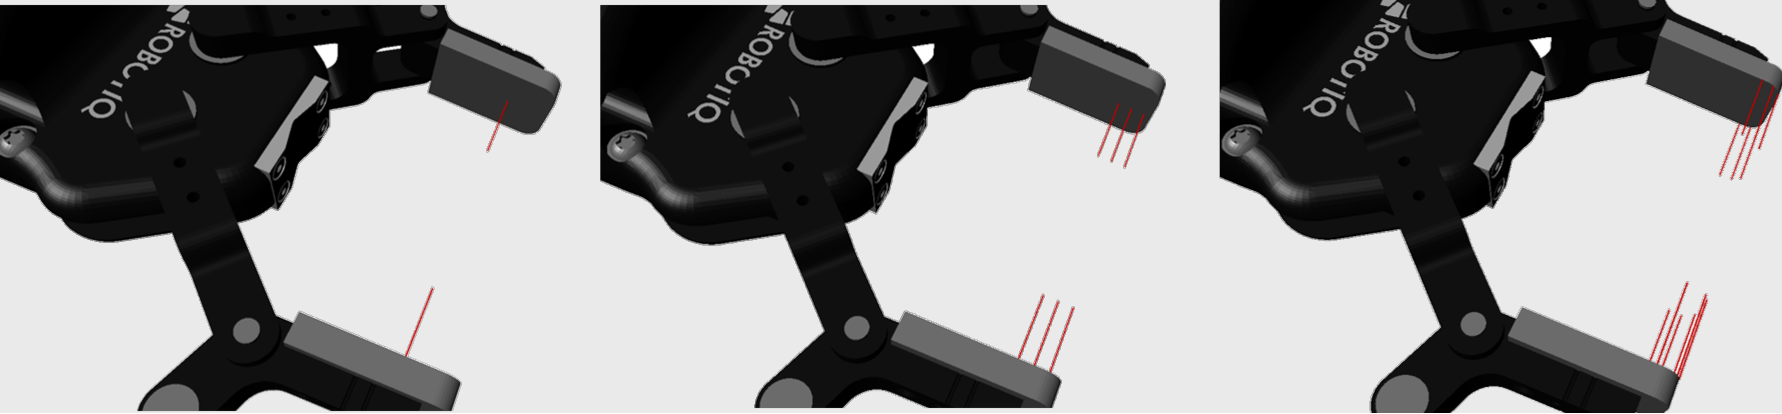
\includegraphics[trim={0cm 0cm 0cm 0cm},clip,width=1\linewidth,angle=0]{Cap5/Figuras/contact_points.pdf}}
\end{tcolorbox}
\caption{Possible configuration of \ac{ICR}. From left to right the number of contact points increases. The model becomes more reliable but convergence of the algorithm is more prone to issues.}
\label{fig:icr}
}%end resize box
\end{figure}

In the presented use cases, the grippers have only one \textit{eingengrasp} (Section~\ref{sec:sim_ann}), simplifying the convergence of the \ac{SANN} algorithm. This approach is adequate to model all joint movement as only one group since the gripper does not have independent fingers and only performs the opening-closing procedure.


The candidate's dataset build starts by setting the active pair for each project. Additionally, a fine-tuning of \ac{SANN} parameters is also configured according to the definitions of Section~\ref{sec:sim_ann} and~\ref{cap4:modular_grasping_architecture:sec:grasping_synthesis:subsec:graspit}. 


%To run the grasping synthesis and initialize the process of Figure~\ref{fig:grasping_graspit_module_workflow}, it is configured each object to be grasped, the gripper type, the $\epsilon$-value (the quality metric used, discussed in Section~\ref{cap2:related_work:sec:grasping_representation}) and the maximum iterations thresholds. A fine-tuning of \ac{SANN} parameters is also setup.


%The Grasping Viewer interface (seen in Figure~\ref{fig:bracket}) shows the progress of grasp finding for each iteration.
%The Figure~\ref{fig:grasping_graspit_module_workflow} present At the end of each \ac{SANN}, a set of good grasps is stored and a new simulation is launched until the maximum iterations are reached. 
After the grasping synthesis process executed all iterations of the optimisation algorithm, the ``Post-processor'' pipeline is called by setting the distance filter, Section~\ref{cap4:modular_grasping_architecture:sec:grasping_synthesis:subsec:postprocessor:subsubsec:distance_filter}, which evaluates all grasping candidates and eliminates redundant grasping poses. This pipeline merges candidates that are close to each other by angular and linear distance based on configurable thresholds. It also deployed the \ac{TCP} angle twin heuristics (Section~\ref{cap4:modular_grasping_architecture:sec:grasping_synthesis:subsec:postprocessor:subsubsec:tcp_angle_twin}) because the grippers are $180^o$ symmetric over attack axis and duplicating each candidate increases the dataset diversity. The object angle twin, Section~\ref{cap4:modular_grasping_architecture:sec:grasping_synthesis:subsec:postprocessor:subsubsec:obj_angle_twin} is also used in the case of symmetric objects, such as falange piece, bearing holder and rod objects. This heuristic saves processing time by avoiding excessive optimisation iterations.

The Figures~\ref{fig:obj_fasten},~\ref{fig:obj_mari4yard} and ~\ref{fig:obj_produtech} elucidate the generated dataset for all projects objects. The candidates are presented in the format of 3D frames over the working object. These dataset are exported in the proposed standard, Section~\ref{cap4:modular_grasping_architecture:sec:grasping_dataset}, and deployed in the robot which will be used by the embedded ``Grasping Selection'' pipeline, in run-time grasping operation.

 \begin{figure}[h!]
 \resizebox{.8\textwidth}{!}{%
 \begin{tcolorbox}
      \centering
      \begin{subfigure}[c]{.23\textwidth}
          \centering
          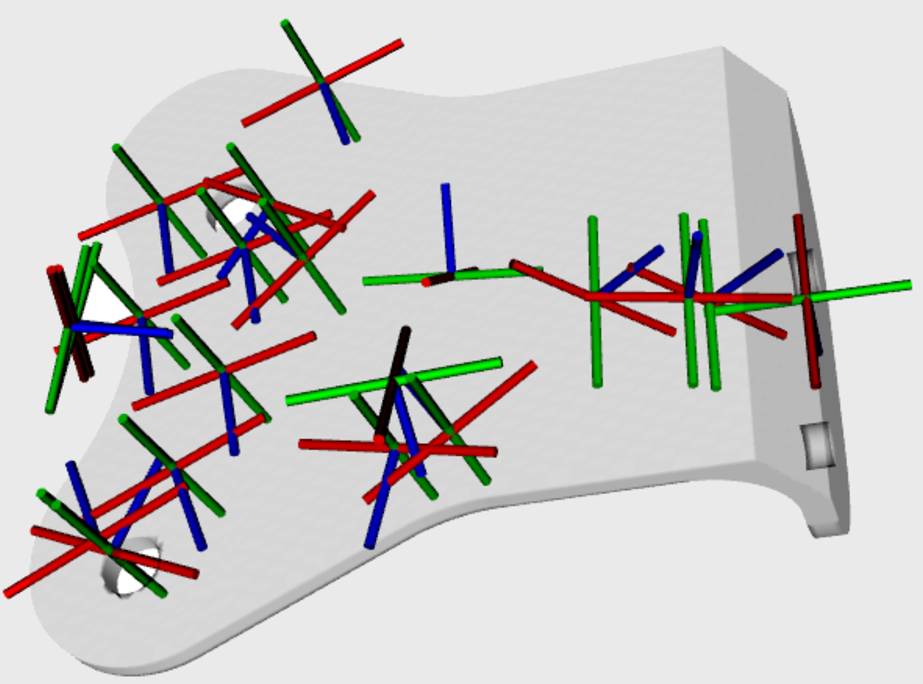
\includegraphics[trim={0cm 0cm 0cm 0cm},clip,width=1\linewidth,angle=0]{Cap5/Figuras/candidates_plot/bracket_candidates.pdf}
          \caption{}
          \label{fig:bracket_candidates}
      \end{subfigure}
      \hfill
      \begin{subfigure}[c]{.23\textwidth}
          \centering
          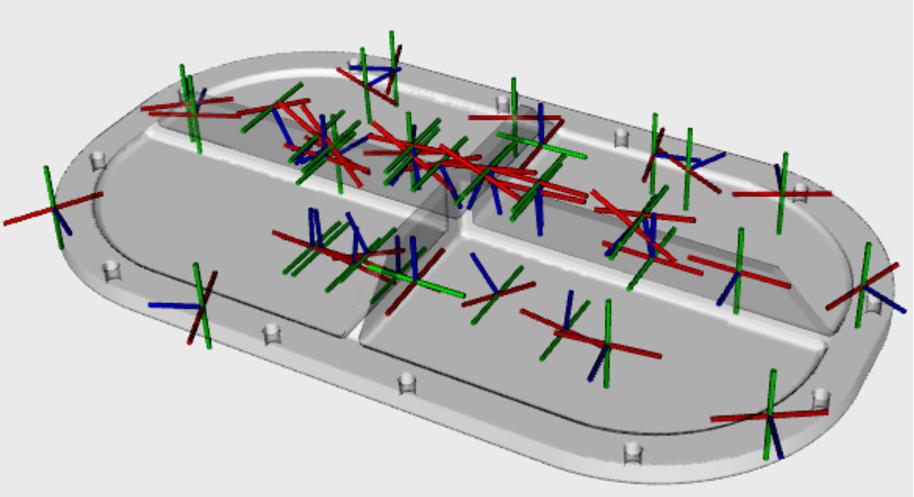
\includegraphics[trim={0cm 0cm 0cm 0cm},clip,width=1\linewidth,angle=0]{Cap5/Figuras/candidates_plot/cover_plate_candidates.pdf}
          \caption{}
          \label{fig:cover_plate_candidates}
      \end{subfigure}
      \hfill
      \begin{subfigure}[c]{.23\textwidth}
          \centering
          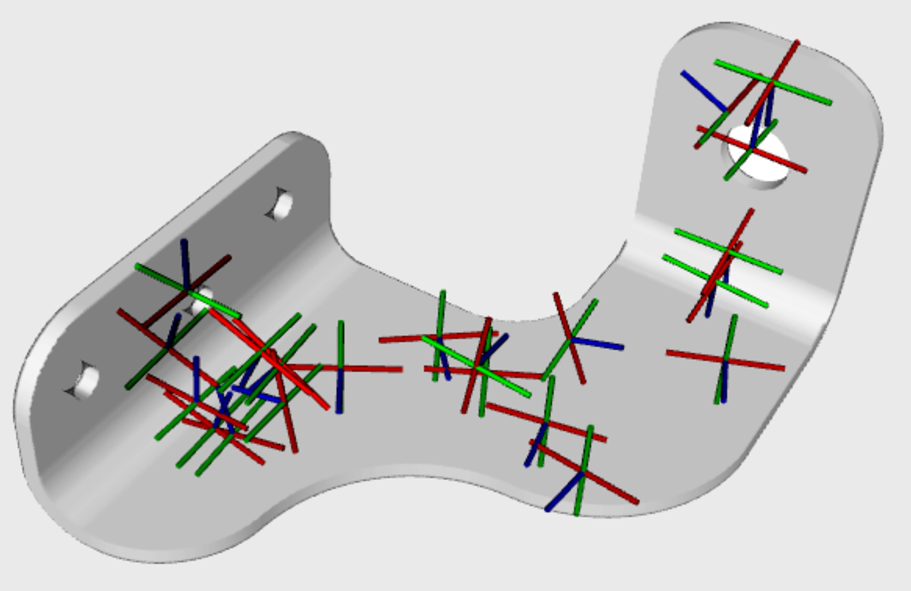
\includegraphics[trim={0cm 0cm 0cm 0cm},clip,width=1\linewidth,angle=0]{Cap5/Figuras/candidates_plot/double_side_bracket_candidates.pdf}
          \caption{}
          \label{fig:double_side_bracket_candidates}
      \end{subfigure}
      \hfill
      \begin{subfigure}[c]{.23\textwidth}
         \centering
         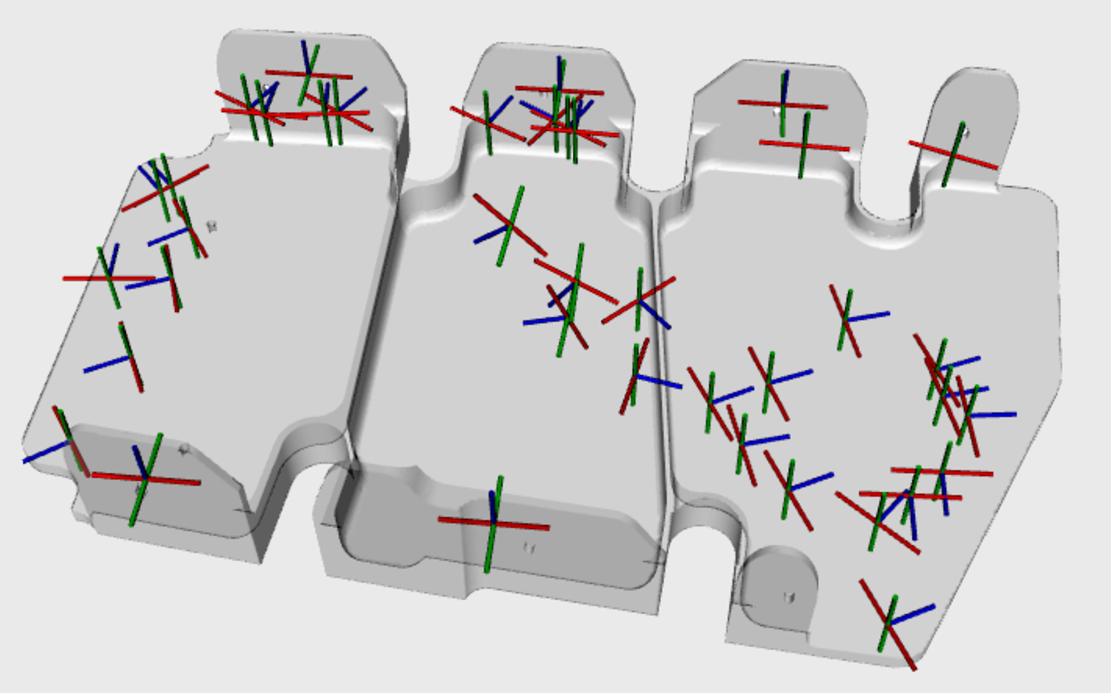
\includegraphics[trim={0cm 0cm 0cm 0cm},clip,width=1\linewidth,angle=0]{Cap5/Figuras/candidates_plot/multi_side_bracket_candidates.pdf}
         \caption{}
         \label{fig:multi_side_bracket_candidates}
      \end{subfigure}
      \hfill
      \begin{subfigure}[c]{.23\textwidth}
         \centering
         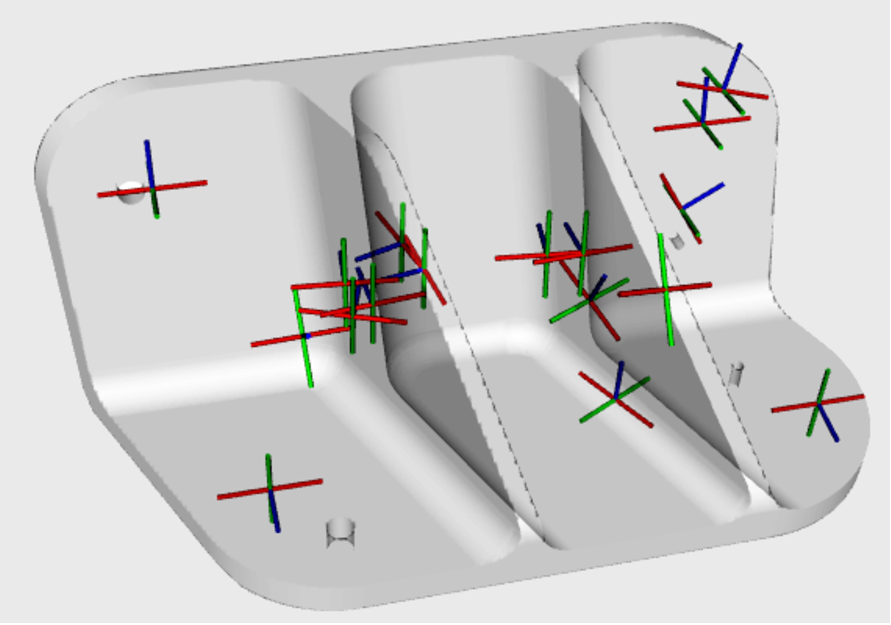
\includegraphics[trim={0cm 0cm 0cm 0cm},clip,width=1\linewidth,angle=0]{Cap5/Figuras/candidates_plot/reinforced_bracket_candidates.pdf}
         \caption{}
         \label{fig:reinforced_bracket_candidates}
      \end{subfigure}
      \hfill
      \begin{subfigure}[c]{.23\textwidth}
         \centering
         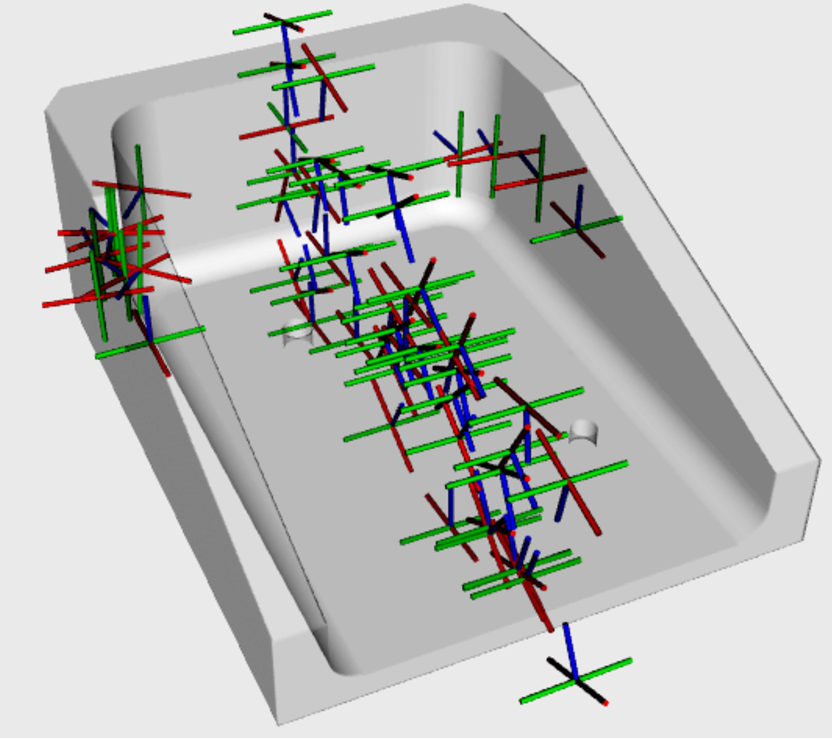
\includegraphics[trim={0cm 0cm 0cm 0cm},clip,width=1\linewidth,angle=0]{Cap5/Figuras/candidates_plot/single_side_bracket_candidates.pdf}
         \caption{}
         \label{fig:single_side_bracket_candidates}
      \end{subfigure}
      \hfill
      \begin{subfigure}[c]{.23\textwidth}
         \centering
         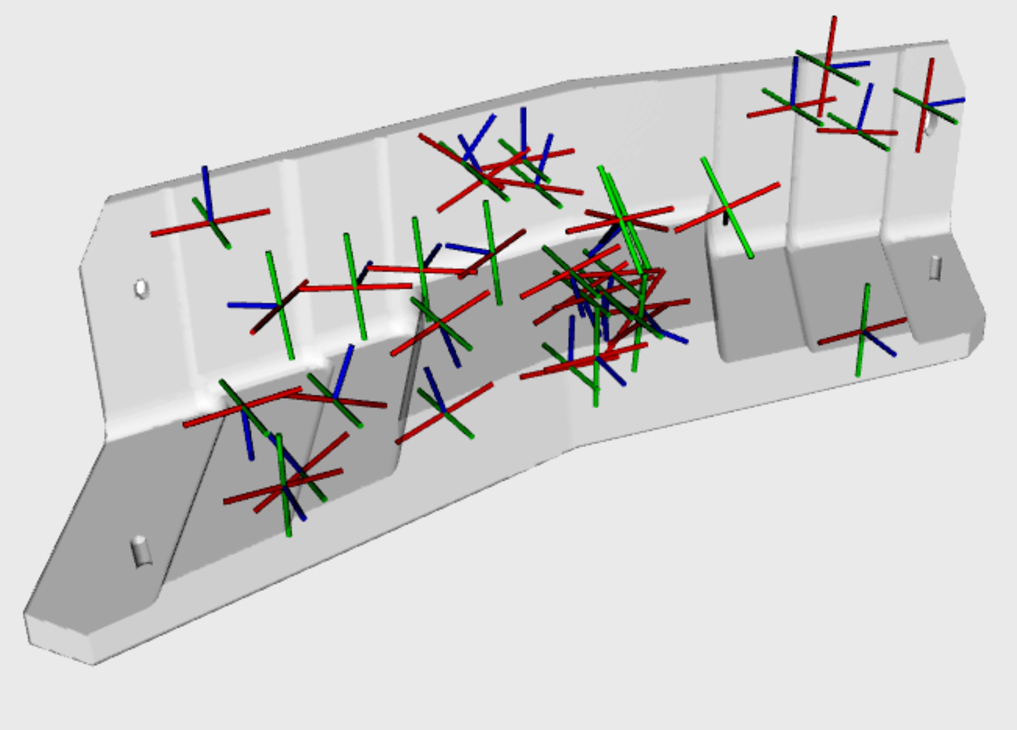
\includegraphics[trim={0cm 0cm 0cm 0cm},clip,width=1\linewidth,angle=0]{Cap5/Figuras/candidates_plot/support_bracket_candidates.pdf}
         \caption{}
         \label{fig:support_bracket_candidates}
      \end{subfigure}
      \hfill
      \begin{subfigure}[c]{.23\textwidth}
         \centering
         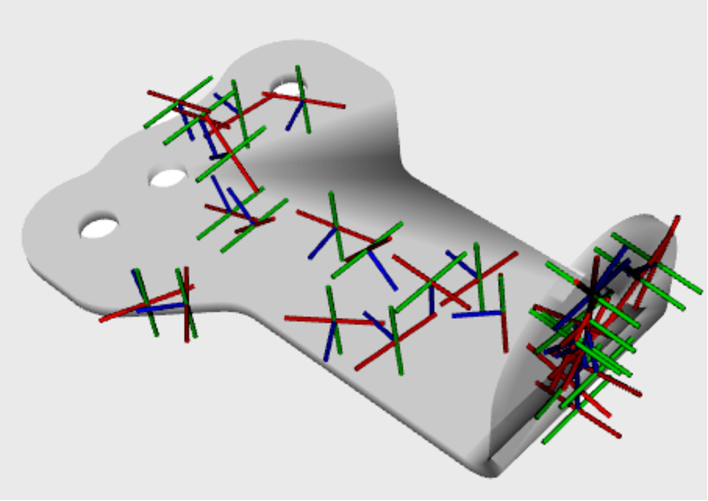
\includegraphics[trim={0cm 0cm 0cm 0cm},clip,width=1\linewidth,angle=0]{Cap5/Figuras/candidates_plot/t_bracket_candidates.pdf}
         \caption{}
         \label{fig:t_bracket_candidates}
      \end{subfigure}
     \end{tcolorbox}
     \caption{Candidates dataset for FASTEN use case.(a) Bracket (b) Cover plate (c) Double side bracket (d) Multi side bracket (e) Reinforced bracket (f) Single side bracket (g) Support bracket (h) T-bracket.}
     \label{fig:obj_candiudates_fasten}
   }%end of resize box      
 \end{figure}
 
 \begin{figure}[h!]
 \resizebox{.8\textwidth}{!}{%
 \begin{tcolorbox}
      \centering
      \begin{subfigure}[c]{.45\textwidth}
          \centering
          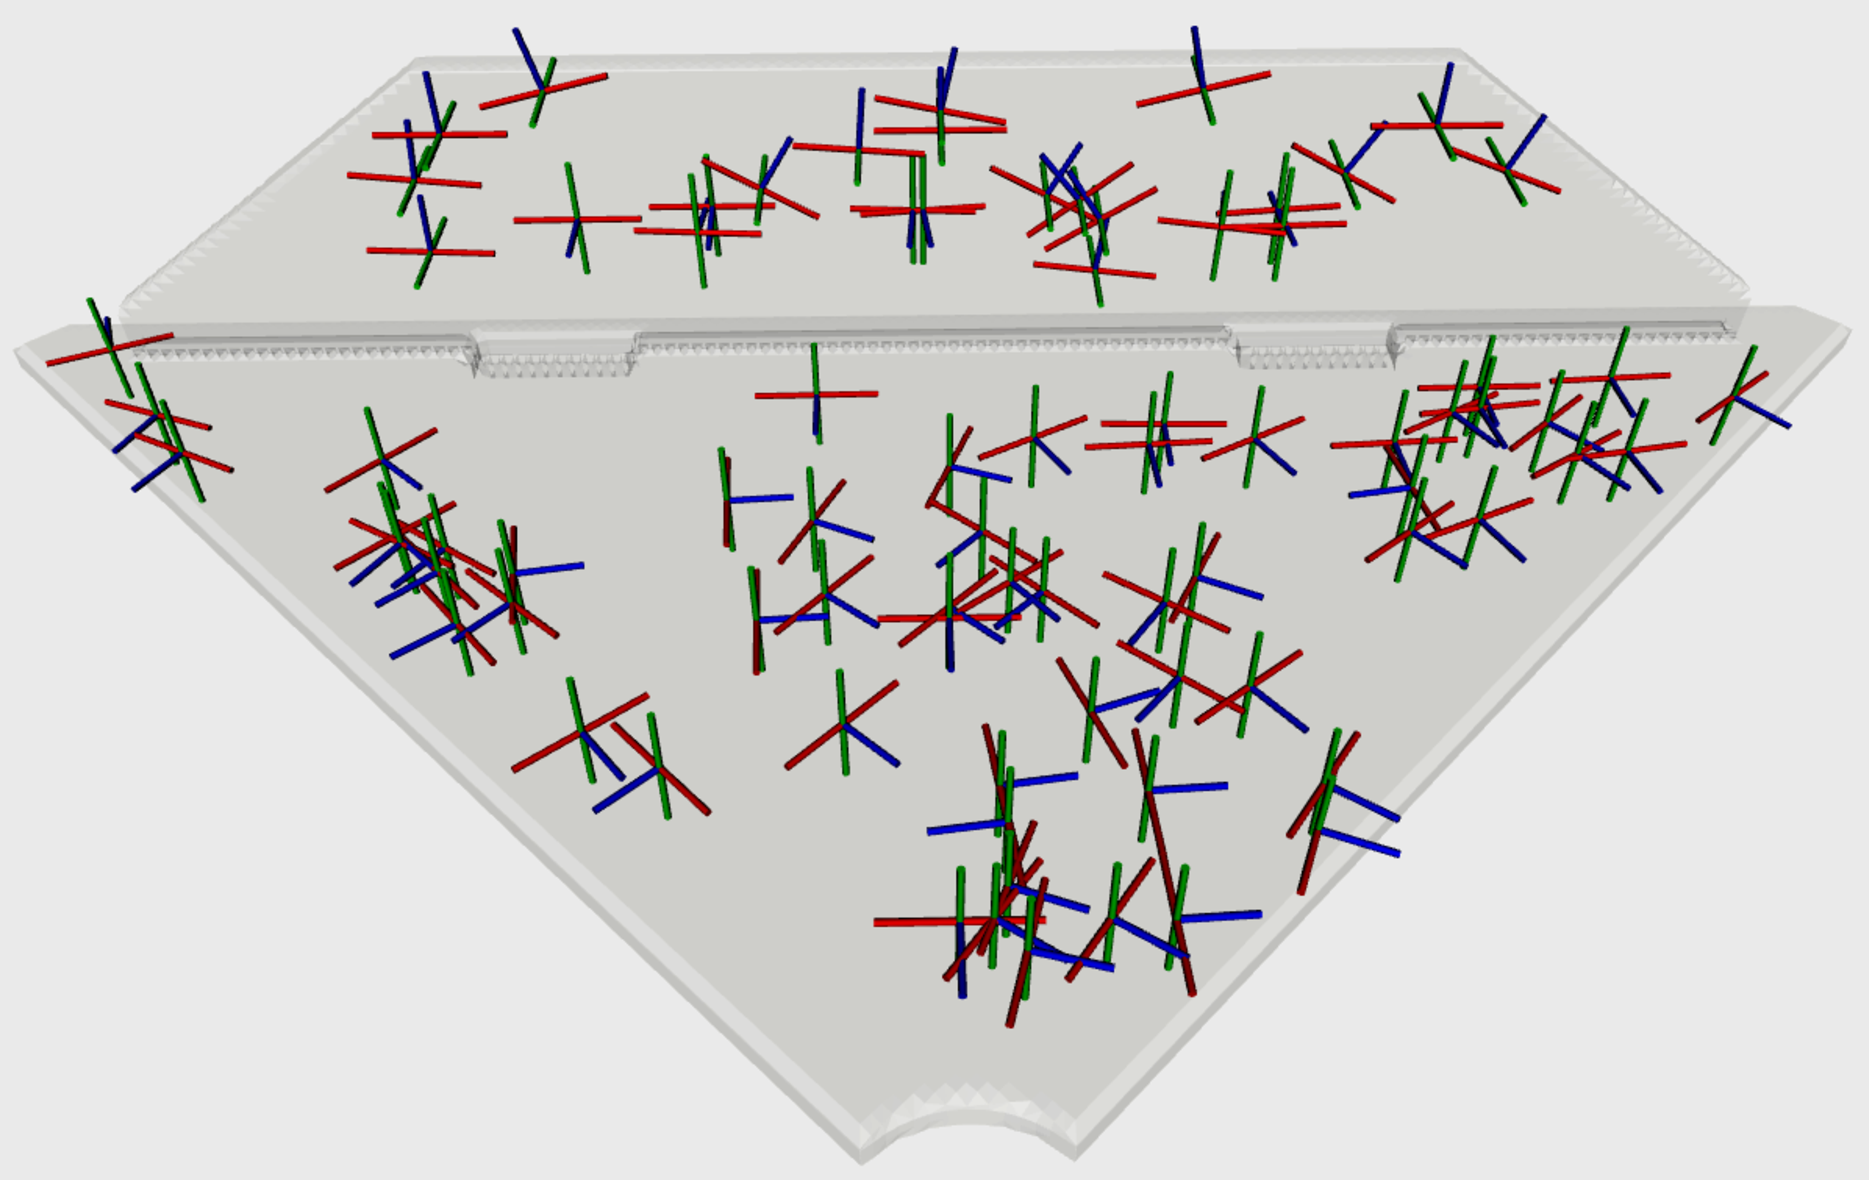
\includegraphics[trim={0cm 0cm 0cm 0cm},clip,width=1\linewidth,angle=0]{Cap5/Figuras/candidates_plot/triangle_bracket_candidates.pdf}
          \caption{}
          \label{fig:triangle_bracket_candidates}
      \end{subfigure}
      \hfill
      \begin{subfigure}[c]{.45\textwidth}
          \centering
          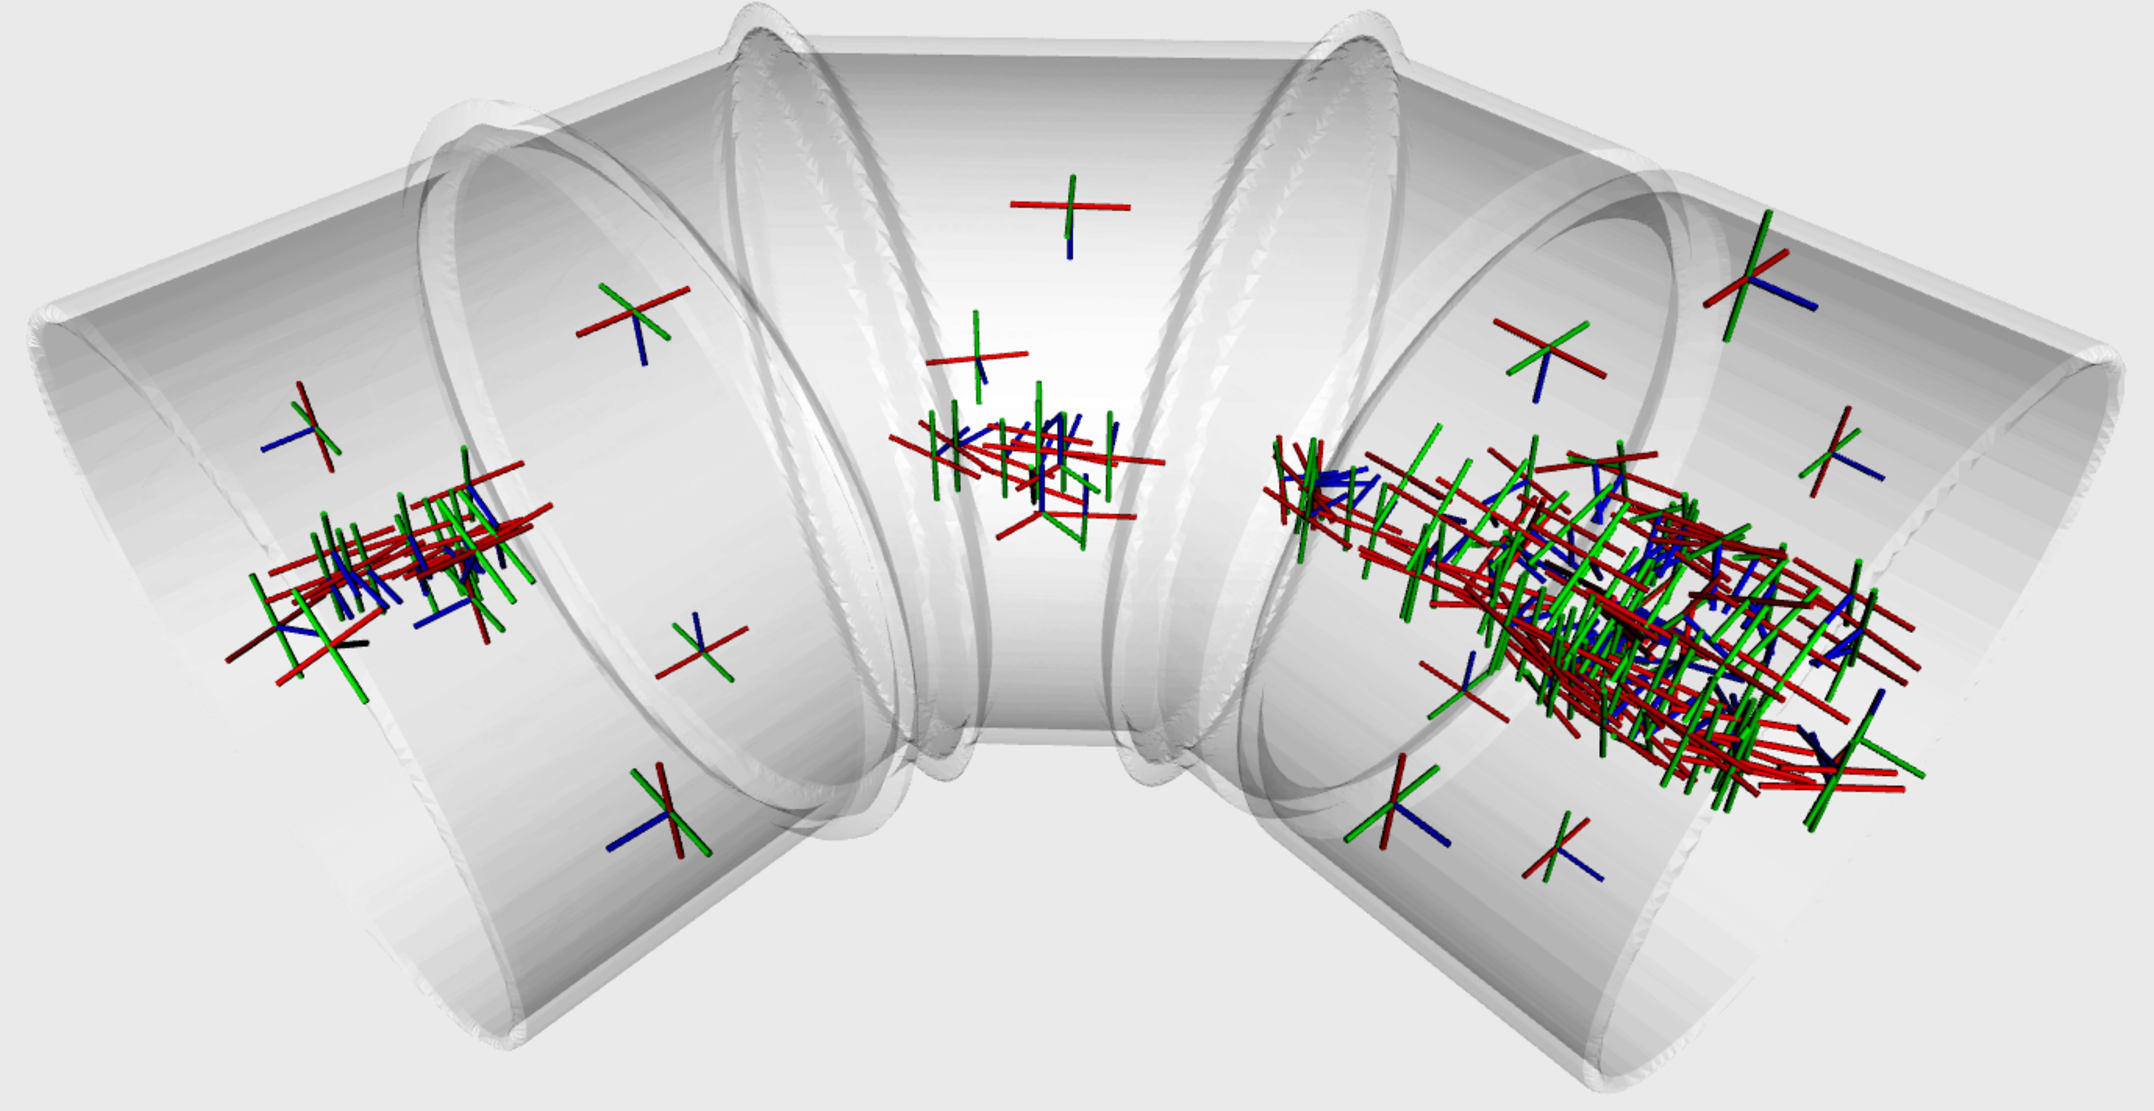
\includegraphics[trim={0cm 0cm 0cm 0cm},clip,width=1\linewidth,angle=0]{Cap5/Figuras/candidates_plot/90_elbow_flue_pipe_candidates.pdf}
          \caption{}
          \label{fig:90_elbow_flue_pipe_candidates}
      \end{subfigure}
     \end{tcolorbox}
     \caption{Candidates dataset for MARI4YARD use case.(a) Triangle bracket (b) 90º elbow flue pipe.}
     \label{fig:obj_candiudates_mari4yard}
   }%end of resize box      
 \end{figure}

 \begin{figure}[h!]
 \resizebox{.75\textwidth}{!}{%
 \begin{tcolorbox}
      \centering
      \begin{subfigure}[c]{.32\textwidth}
          \centering
          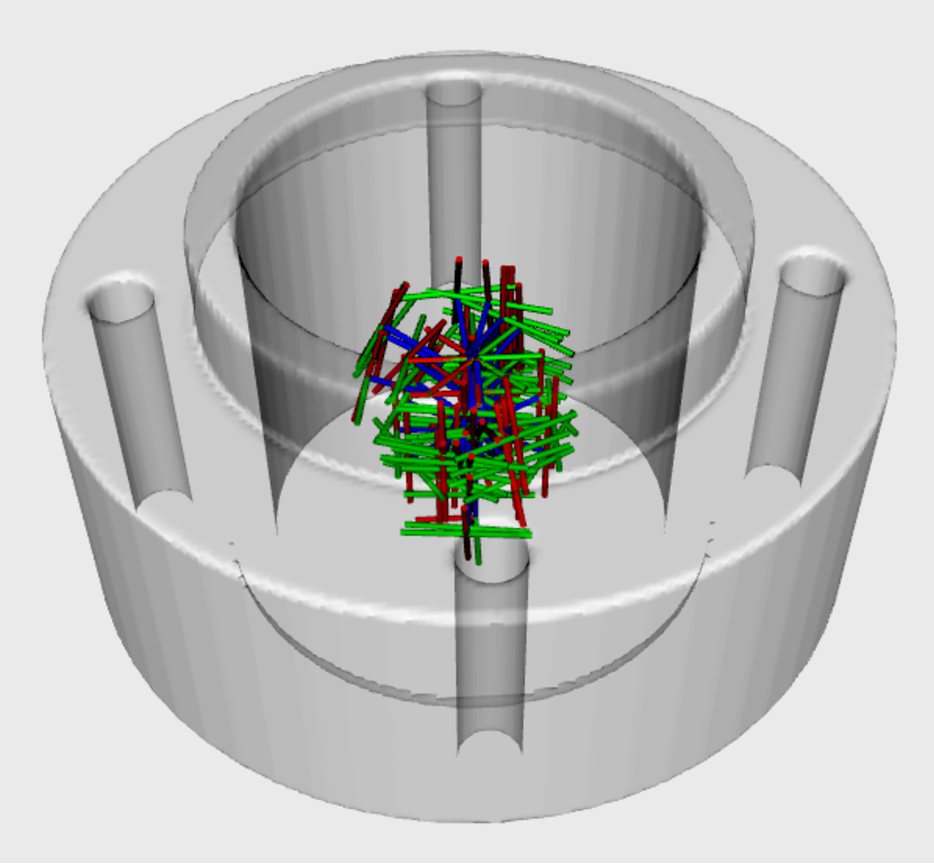
\includegraphics[trim={0cm 0cm 0cm 0cm},clip,width=1\linewidth,angle=0]{Cap5/Figuras/candidates_plot/falange_piece_candidates.pdf}
          \caption{}
          \label{fig:falange_piece_candidates}
      \end{subfigure}
      \hfill
      \begin{subfigure}[c]{.32\textwidth}
          \centering
          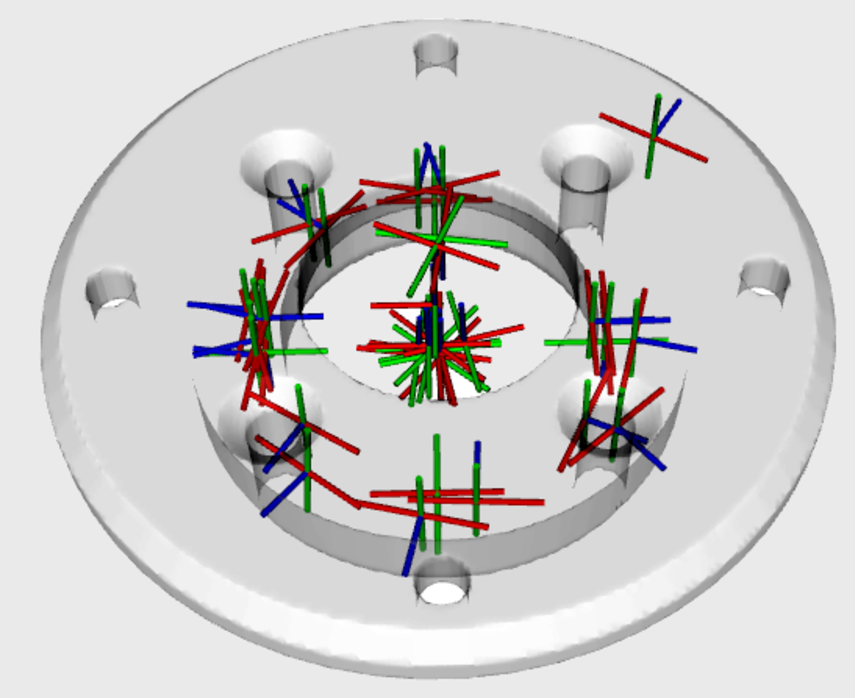
\includegraphics[trim={0cm 0cm 0cm 0cm},clip,width=1\linewidth,angle=0]{Cap5/Figuras/candidates_plot/bearing_holder_candidates.pdf}
          \caption{}
          \label{fig:bearing_holder_candidates}
      \end{subfigure}
      \hfill
      \begin{subfigure}[c]{.125\textwidth}
          \centering
          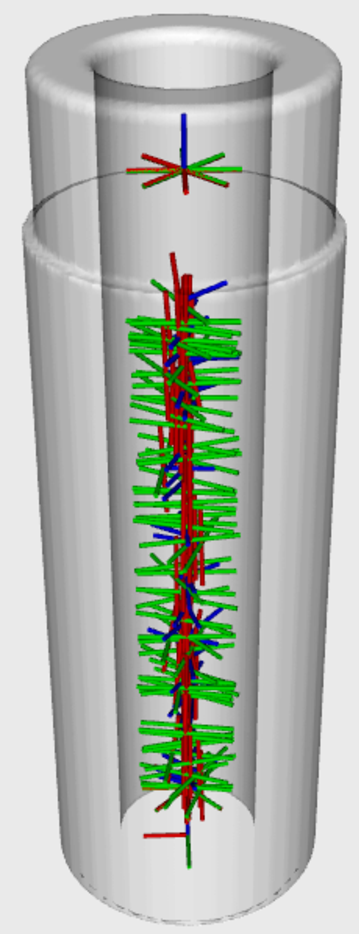
\includegraphics[trim={0cm 0cm 0cm 0cm},clip,width=1\linewidth,angle=0]{Cap5/Figuras/candidates_plot/rod_candidates.pdf}
          \caption{}
          \label{fig:rod_candidates}
      \end{subfigure}
     \end{tcolorbox}
     \caption{Candidates dataset for PRODUTECH 4S\&C use case.(a) Falange piece (b) Bearing holder (c) Rod.}
     \label{fig:obj_candiudates_produtech}
   }%end of resize box      
 \end{figure}

Table~\ref{tab:grasping_synthesis_performance} presents the elapsed time and the candidate dataset's size for each object. The computer setup to build the dataset in Fasten objects is a medium-end computer with 12GB of RAM and 1.80GHz CPU (i7-8550U); for Mari4Yard and Produtech 4S\&C a better-end computer with 16GB of RAM and 2.60GHz CPU (i7-10750H). It is important to note that these PCs are not the ones embedded in the robot. The \ac{SANN} iterations are different according to the size and shape complexity of each piece, e.g. in the case of the multi-side bracket, which possesses small (the seven lateral lumps) and large (the base) graspable surfaces, the \ac{SANN} tends to converge to the largest region, i.e., to the easiest graspable part of the object shape. Therefore, a higher number of iterations may improve the detection of small graspable regions since the initial gripper's position can avoid the recurrence of the minima local problem.

\begin{table}[h!]
\resizebox{.65\textwidth}{!}{%
\begin{tcolorbox}
\centering
\caption{Deployed grasping synthesis performance.}
\label{tab:grasping_synthesis_performance}
\resizebox{1\textwidth}{!}{%
\begin{tabular}{@{}cccc@{}}
\toprule
\textbf{Object}              & \textbf{SA iterations} & \textbf{Elapsed time} & \textbf{Dataset size} \\ \midrule
\textbf{Bracket}             & 30                     & 00:22:33              & 48                    \\
\textbf{Cover plate}         & 30                     & 00:45:07              & 70                    \\
\textbf{Double side bracket} & 30                     & 00:48:04              & 42                    \\
\textbf{Multi side bracket}  & 80                     & 02:38:27              & 150                   \\
\textbf{Reinforced bracket}  & 30                     & 00:39:24              & 37                    \\
\textbf{Single side bracket} & 30                     & 00:42:16              & 83                    \\
\textbf{Support bracket}     & 30                     & 00:32:48              & 44                    \\
\textbf{T-bracket}           & 30                     & 00:34:22              & 46                    \\ \midrule
\textbf{Triangle bracket}    & 50                     & 00:64:43              & 152                   \\
\textbf{90º elbow flue pipe} & 50                     & 00:47:31              & 200                   \\ \midrule
\textbf{Falange piece}       & 50                     & 00:51:52              & 92                    \\
\textbf{Bearing holder}      & 50                     & 00:45:51              & 62                    \\
\textbf{Rod}                 & 50                     & 00:46:54              & 158                   \\ \bottomrule
\end{tabular}%
}
\end{tcolorbox}
}
\end{table}

It is also important to consider the \ac{ICR} model presented in Figure~\ref{fig:icr}. As already mentioned, this affects the algorithm's performance. \ac{ICR}s allocated in the inner part of the gripper could lead the algorithm to not converge. In that case, the fingertip's edge can collide with the object before the \ac{ICR} reaches the contact,  i.e., the \ac{ICR} does not touch the lumps' surface in the case of the multi-side bracket. If many contact points are selected, a contact region larger than the actual grasping region could be originated, and this could lead to a situation where not every contact point belongs to the object. Small \ac{ICR} or \ac{ICR} located very near the fingertip edge instead can generate stable but unpractical grasping. Another source of errors is due to differences between the 3D model used in the Grasp Synthesis stage and the real gripper, see~Figure~\ref{fig:failed_candidates}.

\begin{figure}[h!]
\resizebox{0.6\textwidth}{!}{%
\begin{tcolorbox}
\centerline{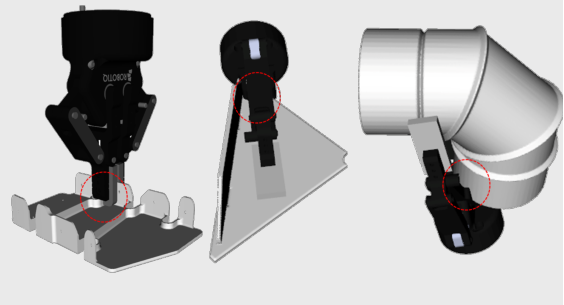
\includegraphics[trim={0cm 0cm 0cm 0cm},clip,width=1\linewidth,angle=0]{Cap5/Figuras/candidates_with_gripper/failed_candidates.pdf}}
\end{tcolorbox}
\caption{Some excluded unfeasible grasping candidates. The unsuspected collisions are highlighted in red circles. These collision is due to 3D model inconsistencies and by the algorithm parameters calibration.}
\label{fig:failed_candidates}
}%end resizebox
\end{figure}

Therefore, it is important that a human supervisor, with the developed grasping viewer ``Post-processor'' (Section~\ref{cap4:modular_grasping_architecture:sec:grasping_synthesis:subsec:postprocessor:subsubsec:viewers}) analyses and selects the grasps hypothesis to be applied in the real scenario. This led to the \ac{GPSR} evaluation proposed in the current thesis where the ground-truth is the human supervisor. The \ac{GPSR} for each used object is presented in Table~\ref{tab:grasping_synthesis_gpsr}. Figure~\ref{fig:candidates_plot} shows some successful example candidates.

%\begin{table}[h!]
%\resizebox{0.25\textwidth}{!}{%
%\begin{tcolorbox}
%\centering
%\caption{Grasping Prediction Success Rate for all used objects.}
%\label{tab:grasping_synthesis_gpsr}
%\resizebox{\textwidth}{!}{%
%\begin{tabular}{@{}cc@{}}
%\toprule
%\textbf{Object}              & \textbf{GPSR} \\ \midrule
%\textbf{Bracket}             & 75\%          \\
%\textbf{Cover plate}         & 97\%          \\
%\textbf{Double side bracket} & 86\%          \\
%\textbf{Multi side bracket}  & 50\%          \\
%\textbf{Reinforced bracket}  & 70\%          \\
%\textbf{Single side bracket} & 100\%         \\
%\textbf{Support bracket}     & 100\%         \\
%\textbf{T-bracket}           & 91\%          \\ \midrule
%\textbf{Triangle bracket}    & 94\%          \\
%\textbf{90º elbow flue pipe} & 97\%          \\ \midrule
%\textbf{Falange piece}       & 100\%         \\
%\textbf{Bearing holder}      & 100\%         \\
%\textbf{Rod}                 & 100\%         \\ \bottomrule
%\end{tabular}%
%}
%\end{tcolorbox}
%}
%\end{table}

\begin{table}[h!]
\centering
\resizebox{1\textwidth}{!}{%
\begin{tcolorbox}
\centering
\caption{Achieved \ac{GPSR} for all use cases.}
\label{tab:grasping_synthesis_gpsr}
\resizebox{1\textwidth}{!}{%
\begin{tabular}{@{}cccccccccccccc@{}}
\toprule
\textbf{Object} &
  \textbf{Bracket} &
  \textbf{\begin{tabular}[c]{@{}c@{}}Cover\\ Plate\end{tabular}} &
  \textbf{\begin{tabular}[c]{@{}c@{}}Double\\ side\\ bracket\end{tabular}} &
  \textbf{\begin{tabular}[c]{@{}c@{}}Multi\\ side\\ bracket\end{tabular}} &
  \textbf{\begin{tabular}[c]{@{}c@{}}Reinforced\\ Bracket\end{tabular}} &
  \textbf{\begin{tabular}[c]{@{}c@{}}Single\\ side\\ bracket\end{tabular}} &
  \textbf{\begin{tabular}[c]{@{}c@{}}Support\\ bracket\end{tabular}} &
  \textbf{T-bracket} &
  \textbf{\begin{tabular}[c]{@{}c@{}}Triangle\\ Bracket\end{tabular}} &
  \textbf{\begin{tabular}[c]{@{}c@{}}90º elbow\\ flue pipe\end{tabular}} &
  \textbf{\begin{tabular}[c]{@{}c@{}}Falange\\ piece\end{tabular}} &
  \textbf{\begin{tabular}[c]{@{}c@{}}Bearing\\ Holder\end{tabular}} &
  \textbf{Rod} \\ \midrule
\textbf{GPSR} &
  75\% &
  97\% &
  86\% &
  70\% &%50\% &
  70\% &
  100\% &
  100\% &
  91\% &
  94\% &
  97\% &
  100\% &
  100\% &
  100\% \\ \bottomrule
\end{tabular}%
}
\end{tcolorbox}
}
\end{table}


 \begin{figure}[h!]
 \resizebox{.75\textwidth}{!}{%
 \begin{tcolorbox}
      \centering
      \begin{subfigure}[c]{1\textwidth}
          \centering
          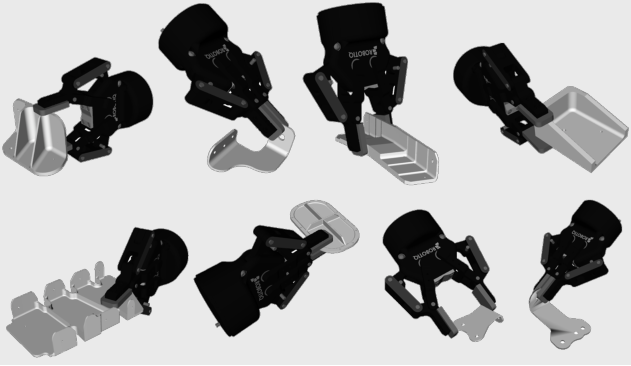
\includegraphics[trim={0cm 0cm 0cm 0cm},clip,width=1\linewidth,angle=0]{Cap5/Figuras/candidates_with_gripper/2f85_candidates.pdf}
          \caption{RobotiQ 2F85 candidates.}
          \label{fig:2f85_candidates}
      \end{subfigure}
      \hfill
      \begin{subfigure}[c]{1\textwidth}
          \centering
          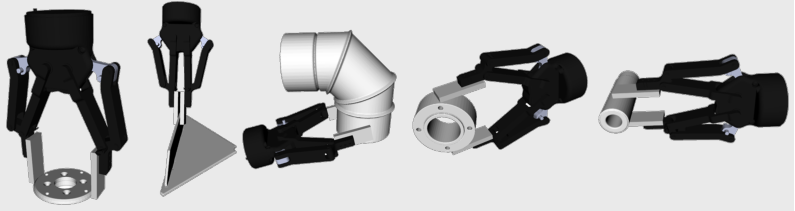
\includegraphics[trim={0cm 0cm 0cm 0cm},clip,width=1\linewidth,angle=0]{Cap5/Figuras/candidates_with_gripper/2f140_candidates.pdf}
          \caption{RobotiQ 2F140 candidates.}
          \label{fig:2f140_candidates}
      \end{subfigure}
     \end{tcolorbox}
     \caption{Candidate examples over Grasp Viewer.}
     \label{fig:candidates_plot}
   }%end of resize box      
 \end{figure}
 

Once the candidate's datasets are built, and the \ac{GPSR} evaluated, the next stage is to deploy them into the robot and assesses the grasping selection pipeline (Section~\ref{cap4:modular_grasping_architecture:sec:grasp_selection}) in run-time operation. The pipeline is configured with the premise of less effort, i.e. euclidean distance, giving preference to near candidates from the \ac{TCP} and roll, pitch yaw movement limit of $-35^o$ to $35^o$, $-35^o$ to $35^o$ and $-180^o$ to $180^o$ w.r.t \ac{TCP}. The workspace filter is used to limit the bin boxes used in all use cases, the workspace cone is limited from the bin box centre to a maximum radius of 55cm and opening of 70º from the normal axis. All values are set empirically. In the end, the joint space filter is applied using the robot URDF model with the gripper in usage in each project and the collision box is calibrated according to it avoiding. For the case of Mari4Yard grasping selection pipeline, the \ac{COG} distance heuristics is also deployed since the objects are bigger and this heuristic improves the \ac{GHSR} and \ac{HGSR} avoiding torque movements between the active-pair. 

A total of 20 grasping attempts were performed on each object. The success rates are presented in Table~\ref{tab:grasping_selection_results}. It is important to note that, if any grasping attempt is failed in some grasping assessment category, this grasping is not considered in the next assessment class, e.g. the reinforced bracket \ac{GRSR} is $95.00\%$, with 19 successful attempts whose define the next the \ac{GHSR} total attempts. In this specific case, the \ac{GHSR} failed in two grasping holding movements, which lead to 17 successes grasping over 19.

\begin{table}[h!]
\resizebox{0.5\textwidth}{!}{%
\begin{tcolorbox}
\centering
\caption{Anchieved \ac{GRSR}, \ac{GHSR} and \ac{HGSR} for the use cases with the proposed pipeline.}
\label{tab:grasping_selection_results}
\resizebox{\textwidth}{!}{%
\begin{tabular}{@{}ccll@{}}
\toprule
\textbf{Object}              & \textbf{GRSR} & \textbf{GHSR}             & \textbf{HGSR}             \\ \midrule
\textbf{Bracket}             & $100\%$   & $85.00\%$ & $100\%$  \\
\textbf{Cover plate}         & $95.00\%$ & $100\%$   & $100\%$   \\
\textbf{Double side bracket} & $100\%$   & $100\%$   & $100\%$   \\
\textbf{Multi side bracket}  & $100\%$     & $95.00\%$    & $100\%$   \\
\textbf{Reinforced bracket}  & $95.00\%$    & $89.47\%$ & $100\%$   \\
\textbf{Single side bracket} & $100\%$   & $100\%$ & $100\%$ \\
\textbf{Support bracket}     & $95.00\%$    & $100\%$   & $100\%$   \\
\textbf{T-bracket}           & $100\%$   & $90.00\%$ & $100\%$   \\ \midrule
\textbf{Triangle bracket}    & $95.00\%$    & $100\%$   & $100\%$   \\
\textbf{90º elbow flue pipe} & $100\%$   & $95.00\%$    & $94.73\%$ \\ \midrule
\textbf{Falange piece}       & $90.00\%$    & $94.44\%$ & $100\%$   \\
\textbf{Bearing holder}      & $95.00\%$    & $100\%$   & $100\%$   \\
\textbf{Rod}                 & $100\%$   & $100\%$   & $100\%$   \\ \bottomrule
\end{tabular}%
}
\end{tcolorbox}
}
\end{table}

An important parameter to be evaluated is the decision time, i.e. the time between the object pose estimation and the candidate selection. These tests were conducted into MariYard and Produtech 4S\&C pieces and presented in Table~\ref{tab:grasping_selection_time}. A priori, the tests were performed with direct estimation method (Section~\ref{cap4:modular_grasping_architecture:sec:grasp_selection}) leading to the decision time of first table column. However, it was verified that the grasping dataset loading into robot memory consumes a large fraction of the total elapsed time. Using the ``pre-load'' ``Grasping Selection'' function, it was verified a considered reduction in these times led to the table's second column values. The elapsed times presented in the table are run-time applicable processing times in comparison with the ``Grasping Synthesis'' achieved time, Table~\ref{tab:grasping_synthesis_performance}, justifying the strategy to divide the overall grasping planner into offline and run-time pipeline strategies.

\begin{table}[h!]
\resizebox{0.5\textwidth}{!}{%
\begin{tcolorbox}
\centering
\caption{Grasping Selection elapsed decision time.}
\label{tab:grasping_selection_time}
\resizebox{\textwidth}{!}{%
\begin{tabular}{@{}ccc@{}}
\toprule
\multirow{2}{*}{\textbf{Object}} &
  \multicolumn{2}{c}{\textbf{Elapsed Decision Time {[}s{]}}} \\ \cmidrule(l){2-3} 
 &
  \textbf{\begin{tabular}[c]{@{}c@{}}Direct \\ Estimation\end{tabular}} &
  \textbf{\begin{tabular}[c]{@{}c@{}}Pre-load Support\\ Estimation\end{tabular}} \\ \midrule
\textbf{Triangle bracket}    & 1.786 & 0.121 \\
\textbf{90º elbow flue pipe} & 2.516 & 0.105 \\ \midrule
\textbf{Falange piece}       & 1.197 & 0.049 \\
\textbf{Bearing holder}      & 0.853 & 0.041 \\
\textbf{Rod}                 & 1.871 & 0.078 \\ \bottomrule
\end{tabular}%
}
\end{tcolorbox}
}
\end{table}


Finally, the Figure~\ref{fig:demo_mari4yard} presents the proposed pipeline applied into the Mari4Yard bin-picking demonstrator. The Figure~\ref{fig:embraer_result} shows the success robot grasping results in Embraer Portugal facilities. %The complete mission video can be verified at \textbf{TODO}


 \begin{figure}[h!]
 \resizebox{0.65\textwidth}{!}{%
 \begin{tcolorbox}
      \centering
      \begin{subfigure}[c]{1\textwidth}
          \centering
          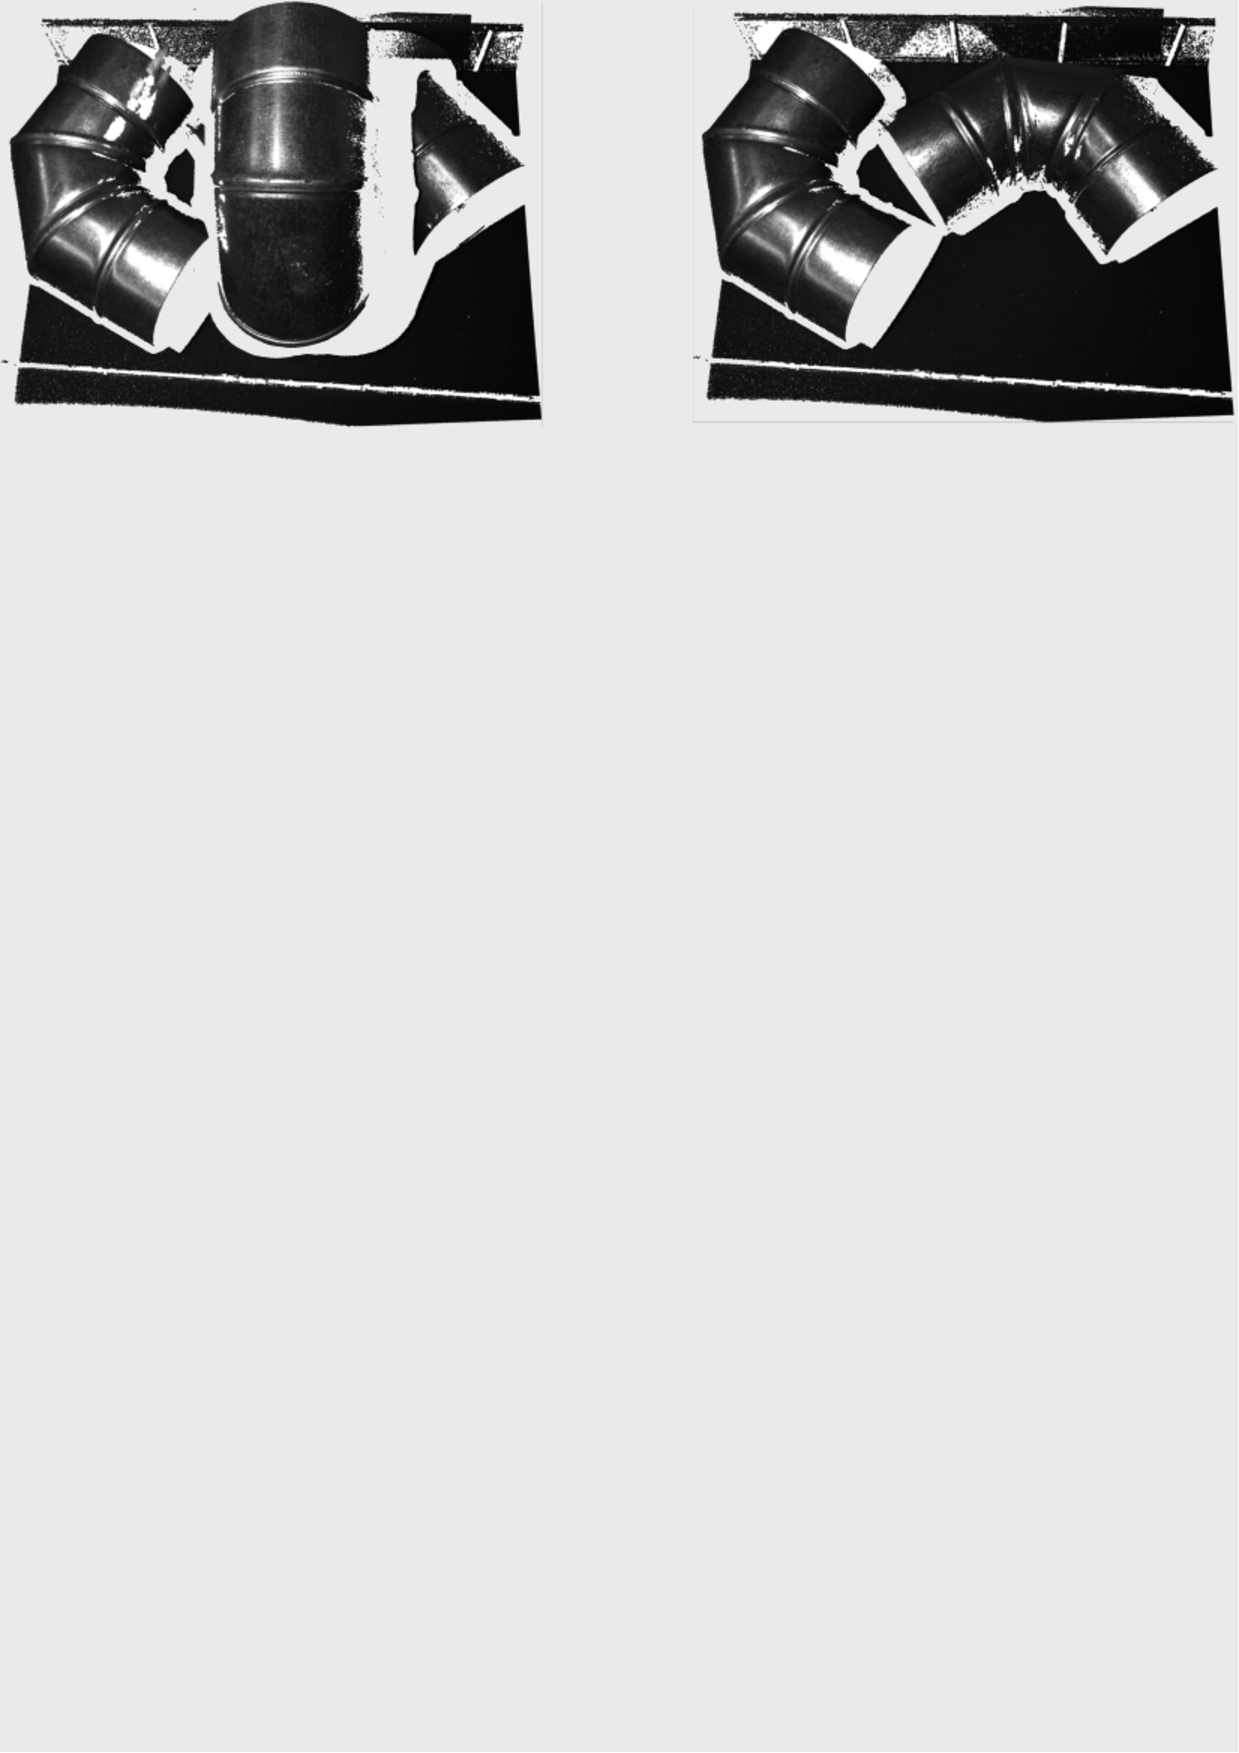
\includegraphics[trim={0cm 23cm 0cm 0cm},clip,width=1\linewidth,angle=0]{Cap5/Figuras/picking_mari4yard/capture_image.pdf}
          \caption{Scene point cloud image.}
          \label{fig:bracket}
      \end{subfigure}
      \hfill
      \begin{subfigure}[c]{1\textwidth}
          \centering
          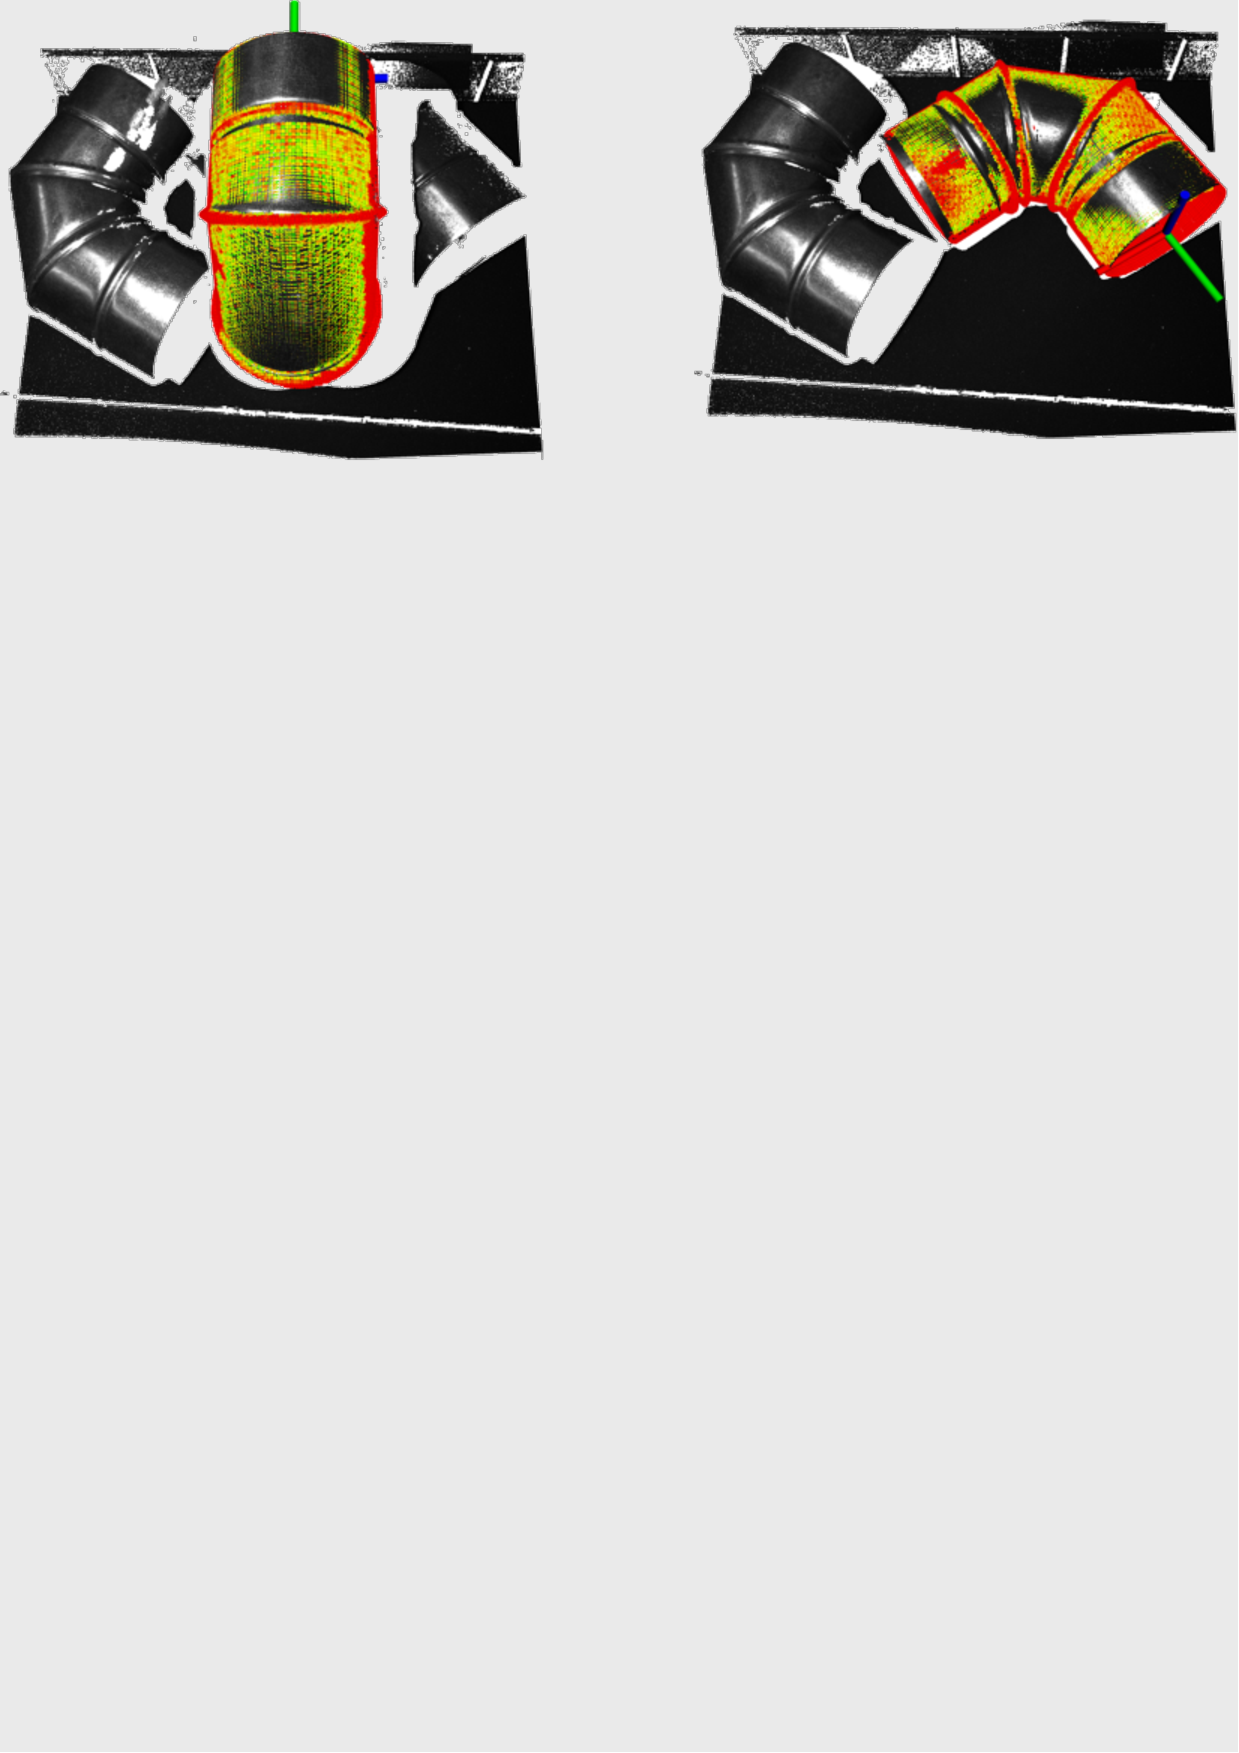
\includegraphics[trim={0cm 23cm 0cm 0cm},clip,width=1\linewidth,angle=0]{Cap5/Figuras/picking_mari4yard/object_detection.pdf}
          \caption{Object pose estimation.}
          \label{fig:cover_plate}
      \end{subfigure}
      \hfill
      \begin{subfigure}[c]{1\textwidth}
          \centering
          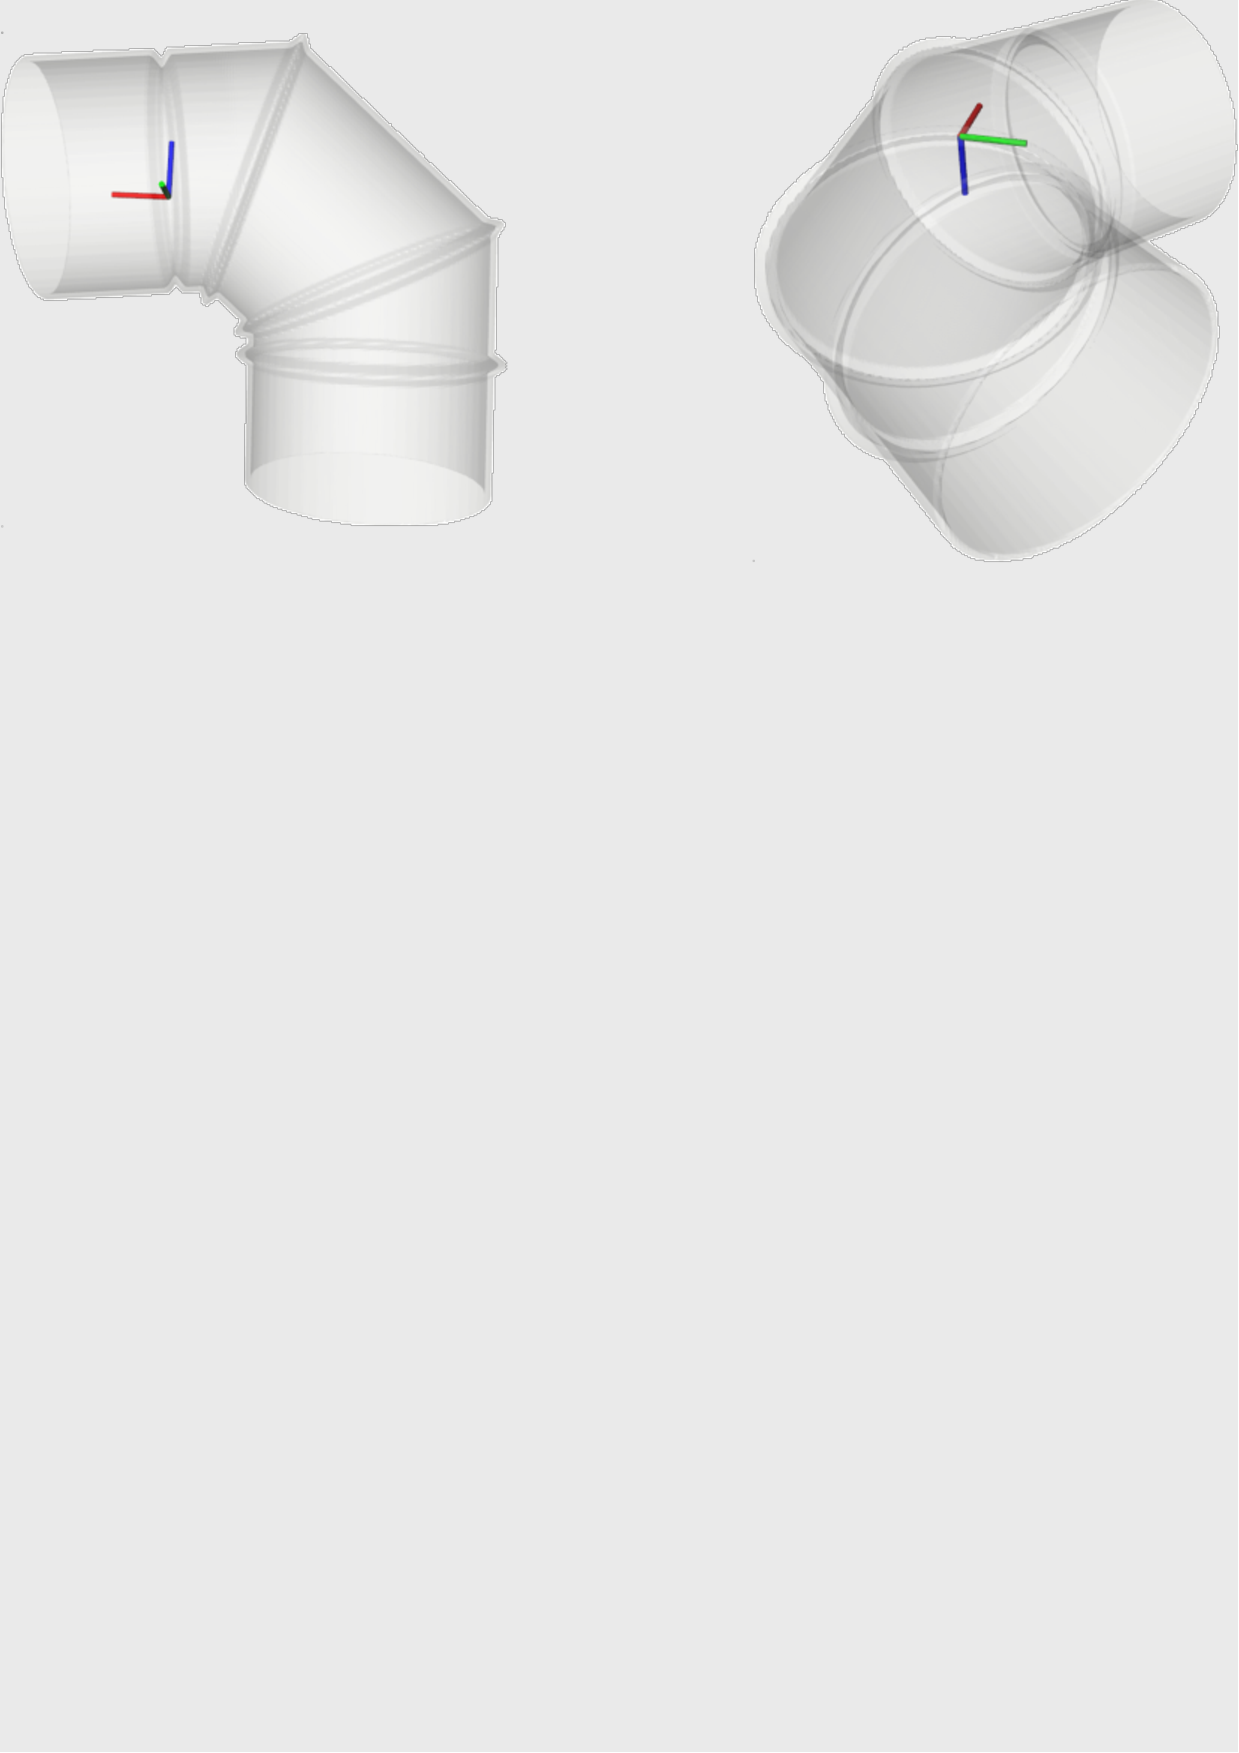
\includegraphics[trim={0cm 20cm 0cm 0cm},clip,width=1\linewidth,angle=0]{Cap5/Figuras/picking_mari4yard/grasping_selection.pdf}
          \caption{Grasping selection pipeline choosing the best candidate.}
          \label{fig:Double_side_bracket}
      \end{subfigure}
      \hfill
      \begin{subfigure}[c]{1\textwidth}
         \centering
          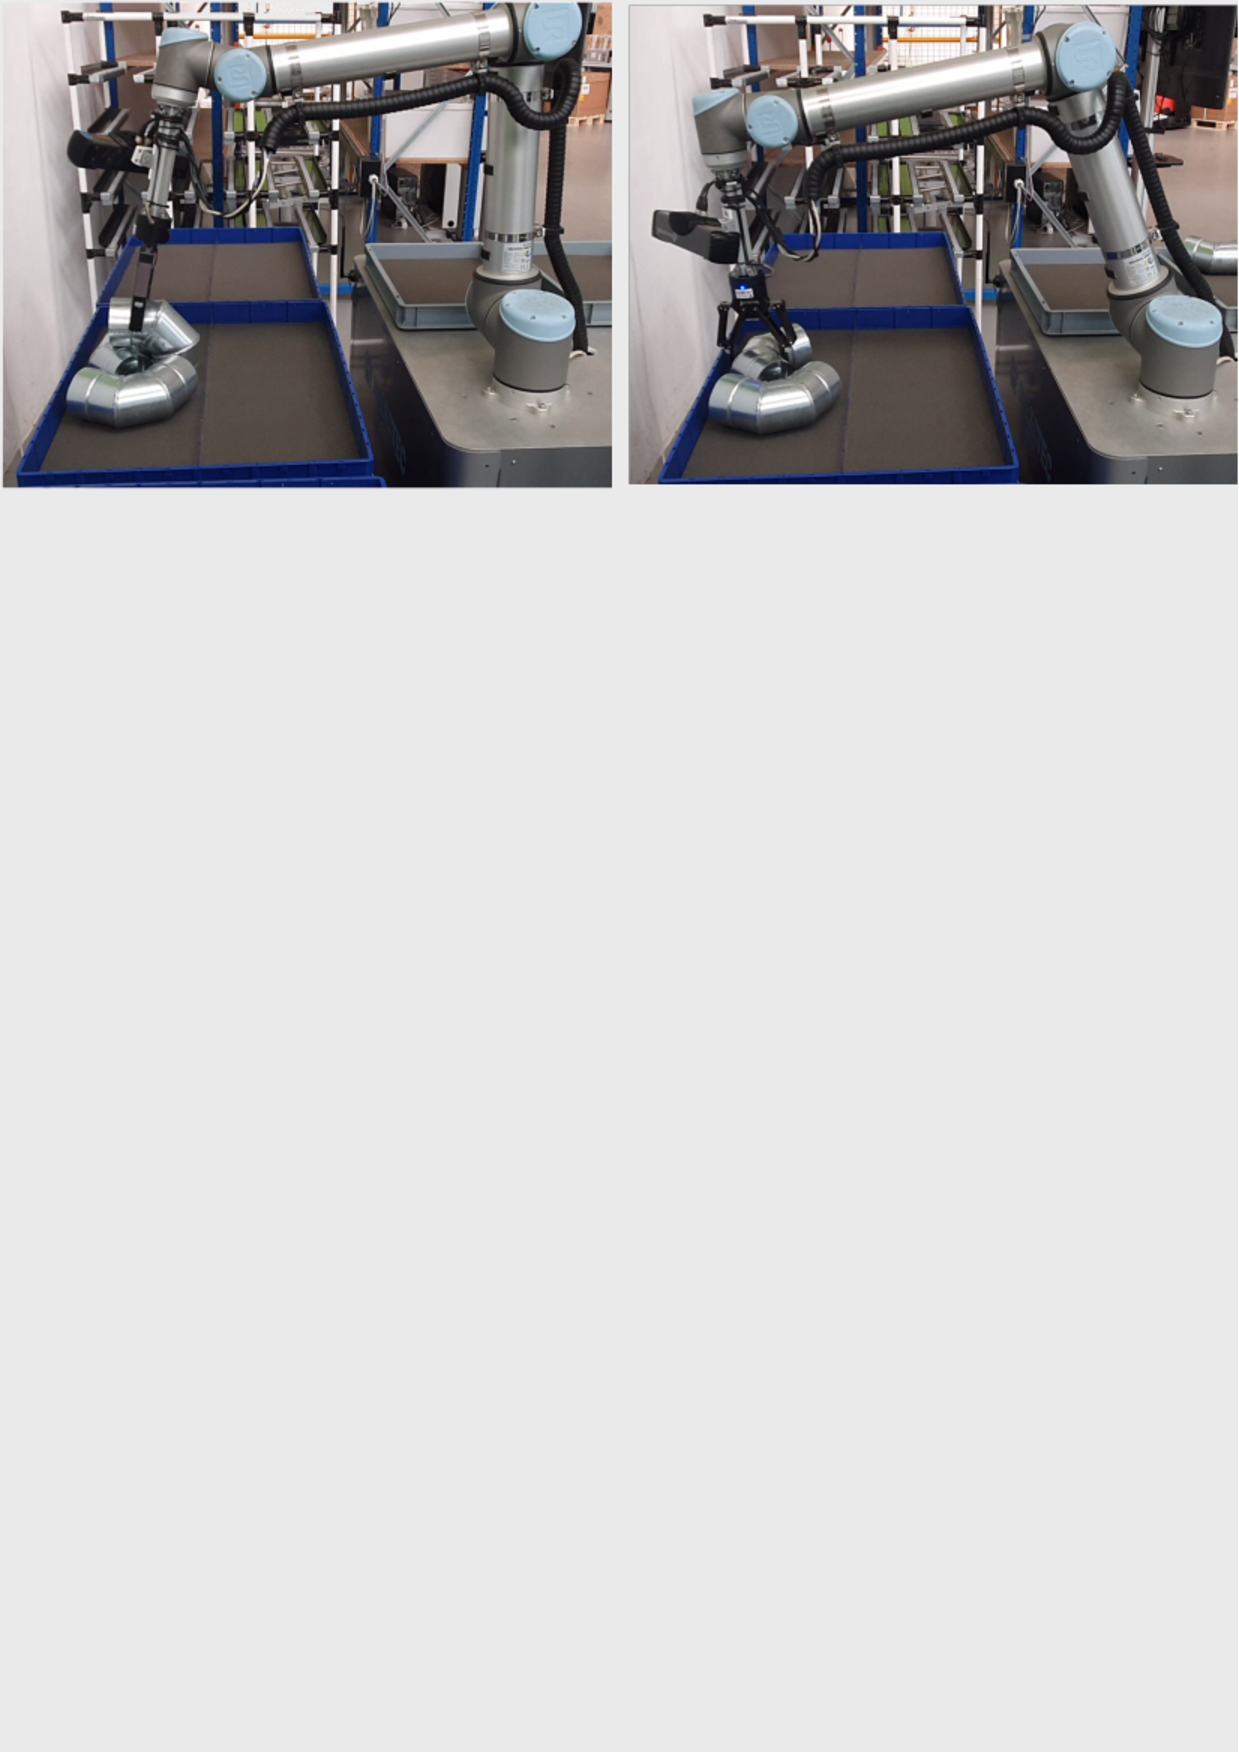
\includegraphics[trim={0cm 22cm 0cm 0cm},clip,width=1\linewidth,angle=0]{Cap5/Figuras/picking_mari4yard/grasping.pdf}
         \caption{The grasping procedure.}
         \label{fig:multi_side_bracket}
      \end{subfigure}
     \end{tcolorbox}
     \caption{Mari4Yard bin-picking demonstrator.}
     \label{fig:demo_mari4yard}
   }%end of resize box      
 \end{figure}

\begin{figure}[h!]
	\resizebox{0.75\textwidth}{!}{%
    \begin{tcolorbox}
    \centering
	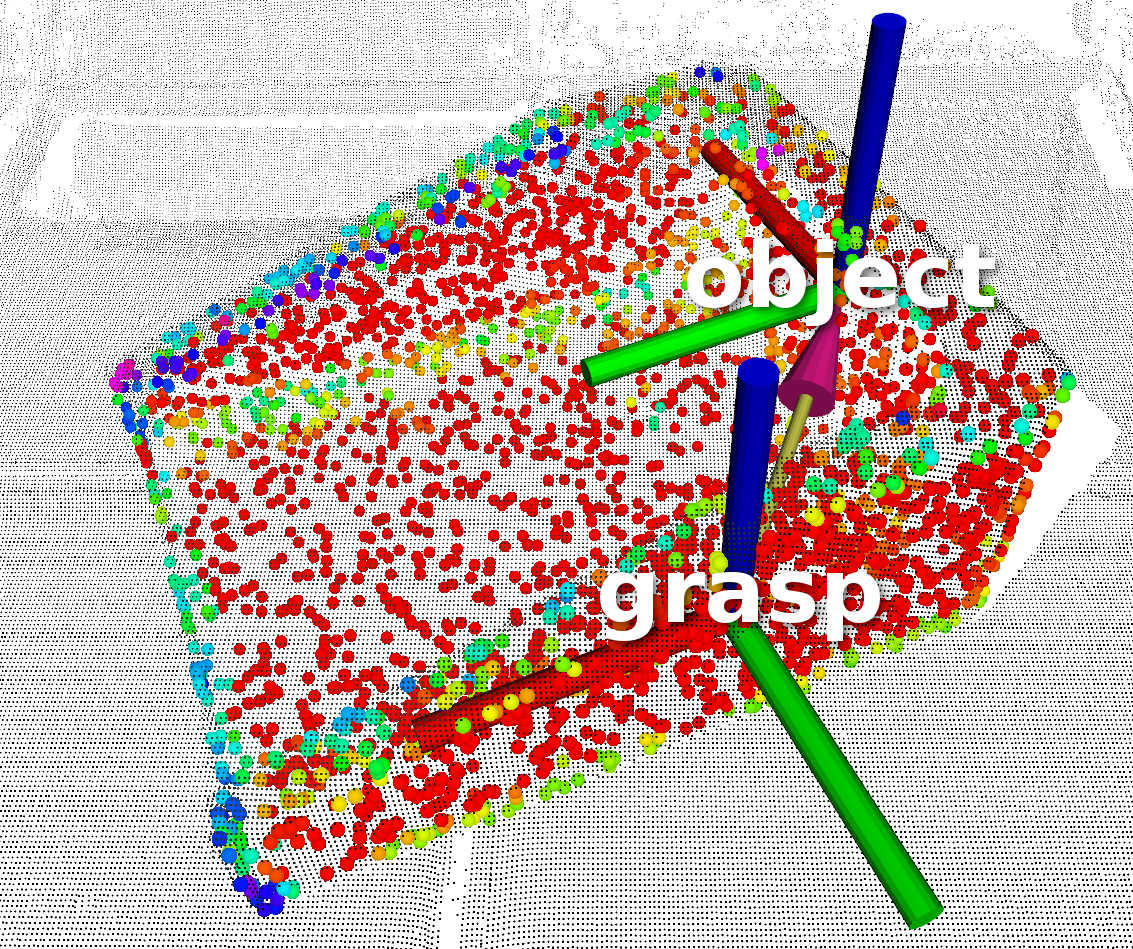
\includegraphics[height=.15\textheight]{Cap5/Figuras/picking_embraer//perception-1}
	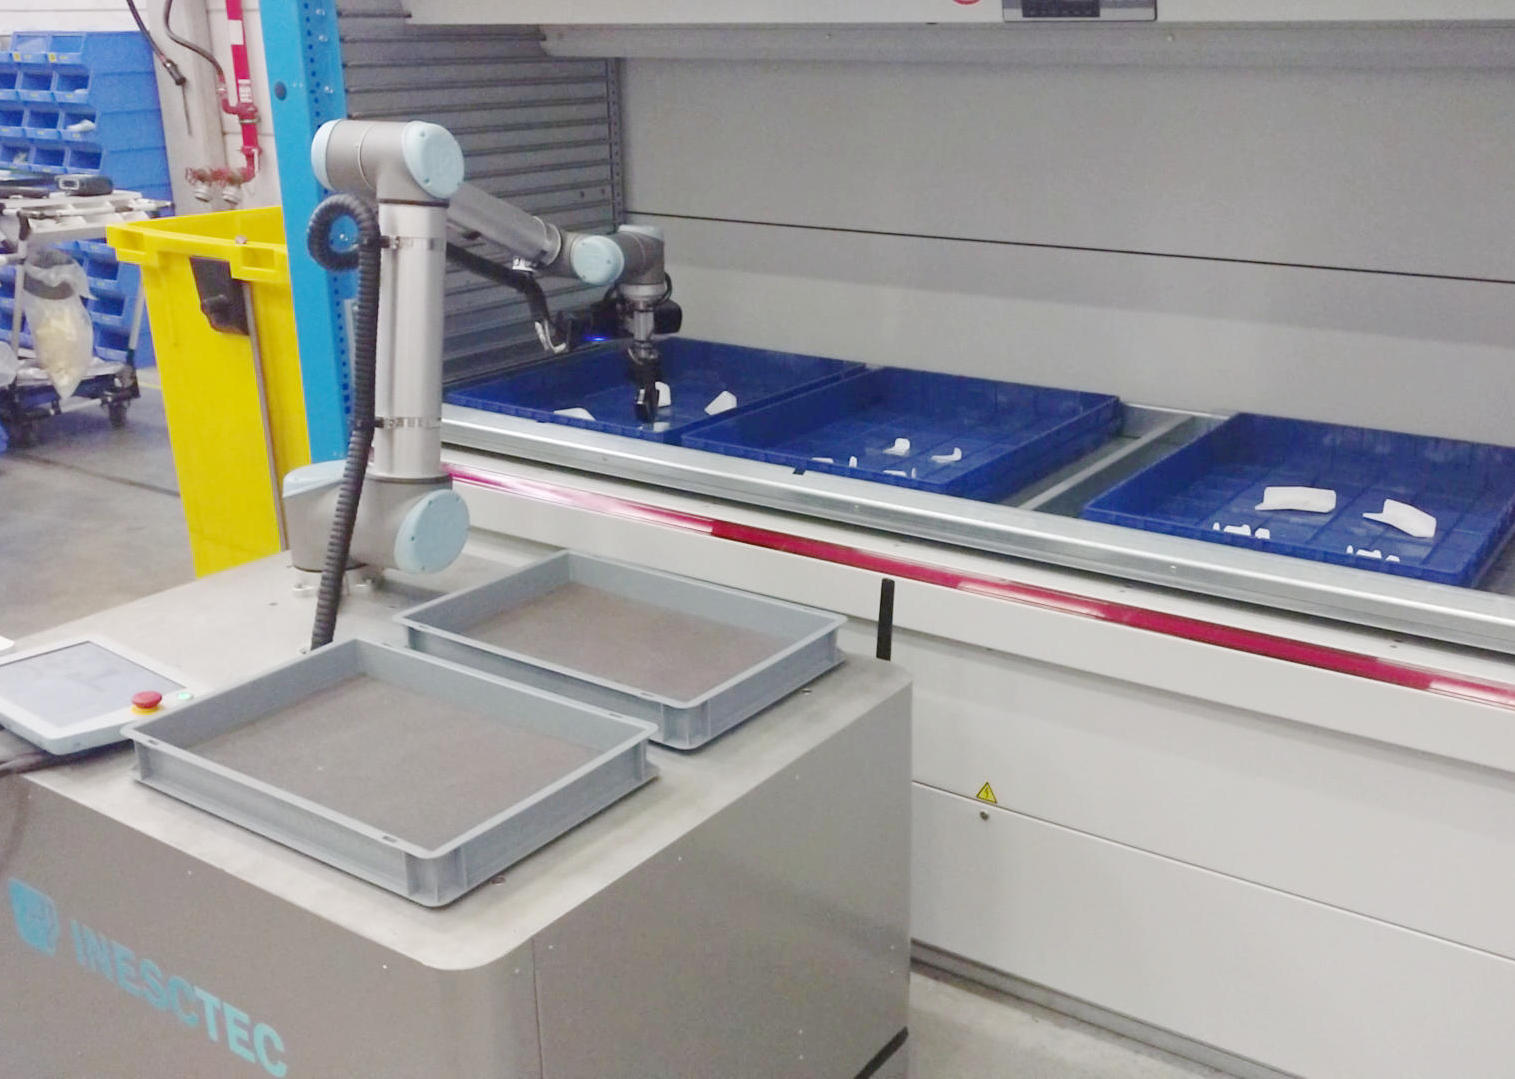
\includegraphics[height=.15\textheight]{Cap5/Figuras/picking_embraer/back-1}
	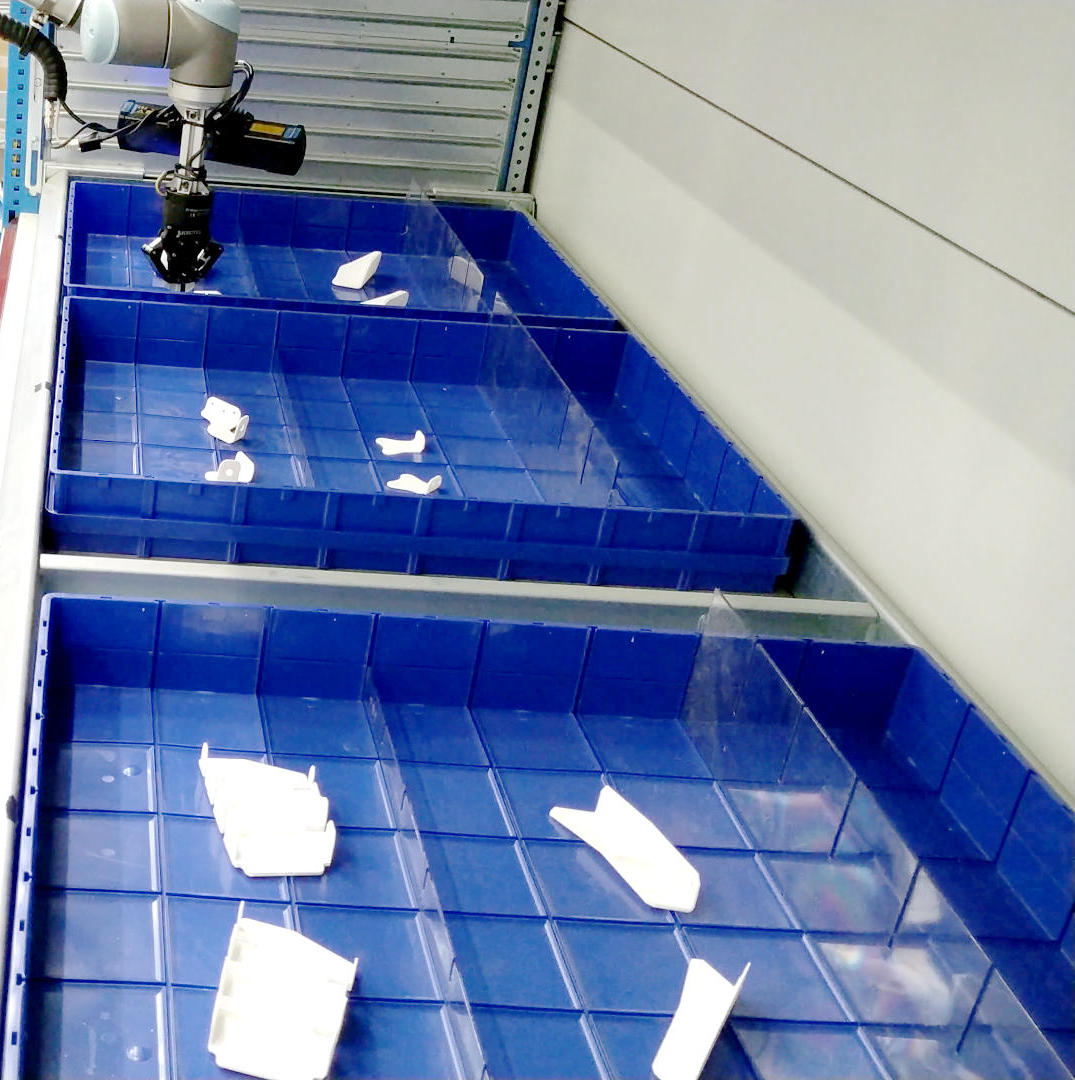
\includegraphics[height=.15\textheight]{Cap5/Figuras/picking_embraer/side-1}\\
	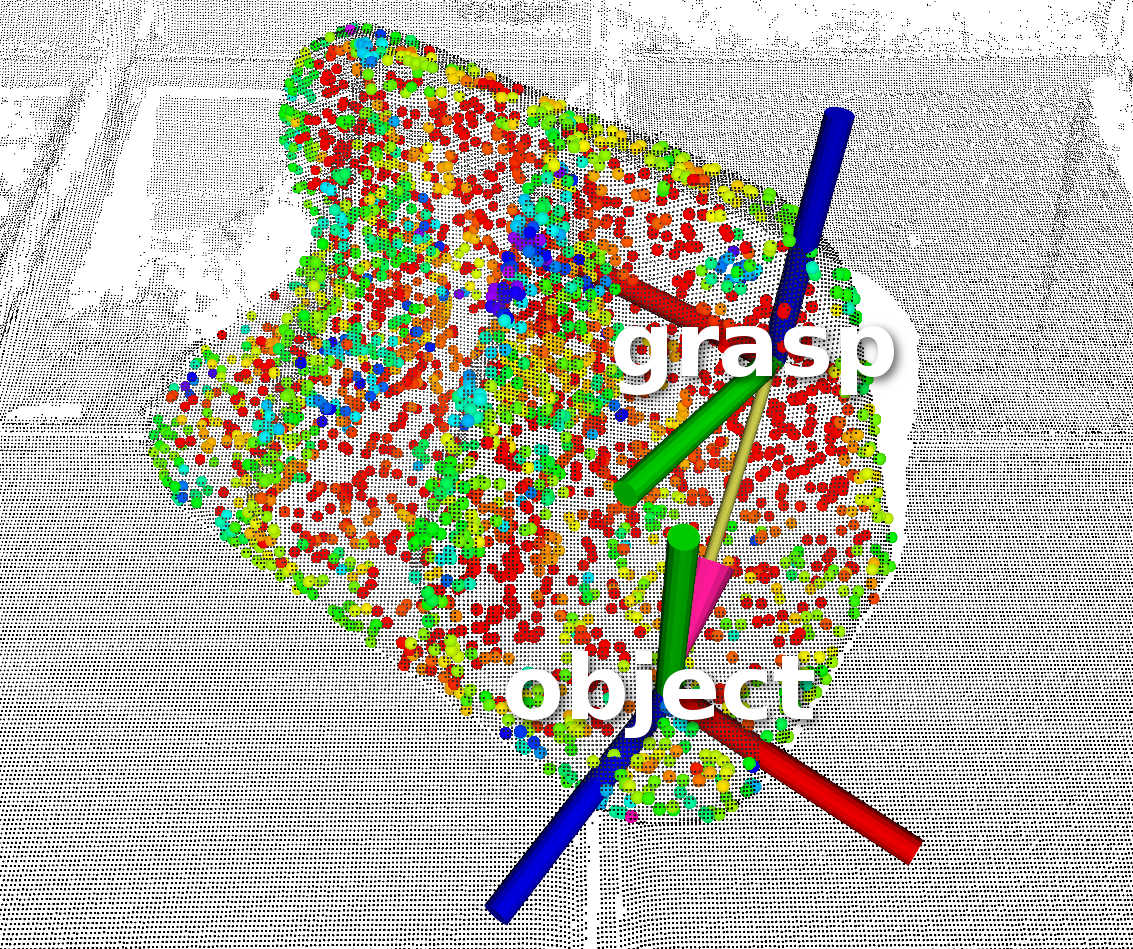
\includegraphics[height=.15\textheight]{Cap5/Figuras/picking_embraer/perception-2}
	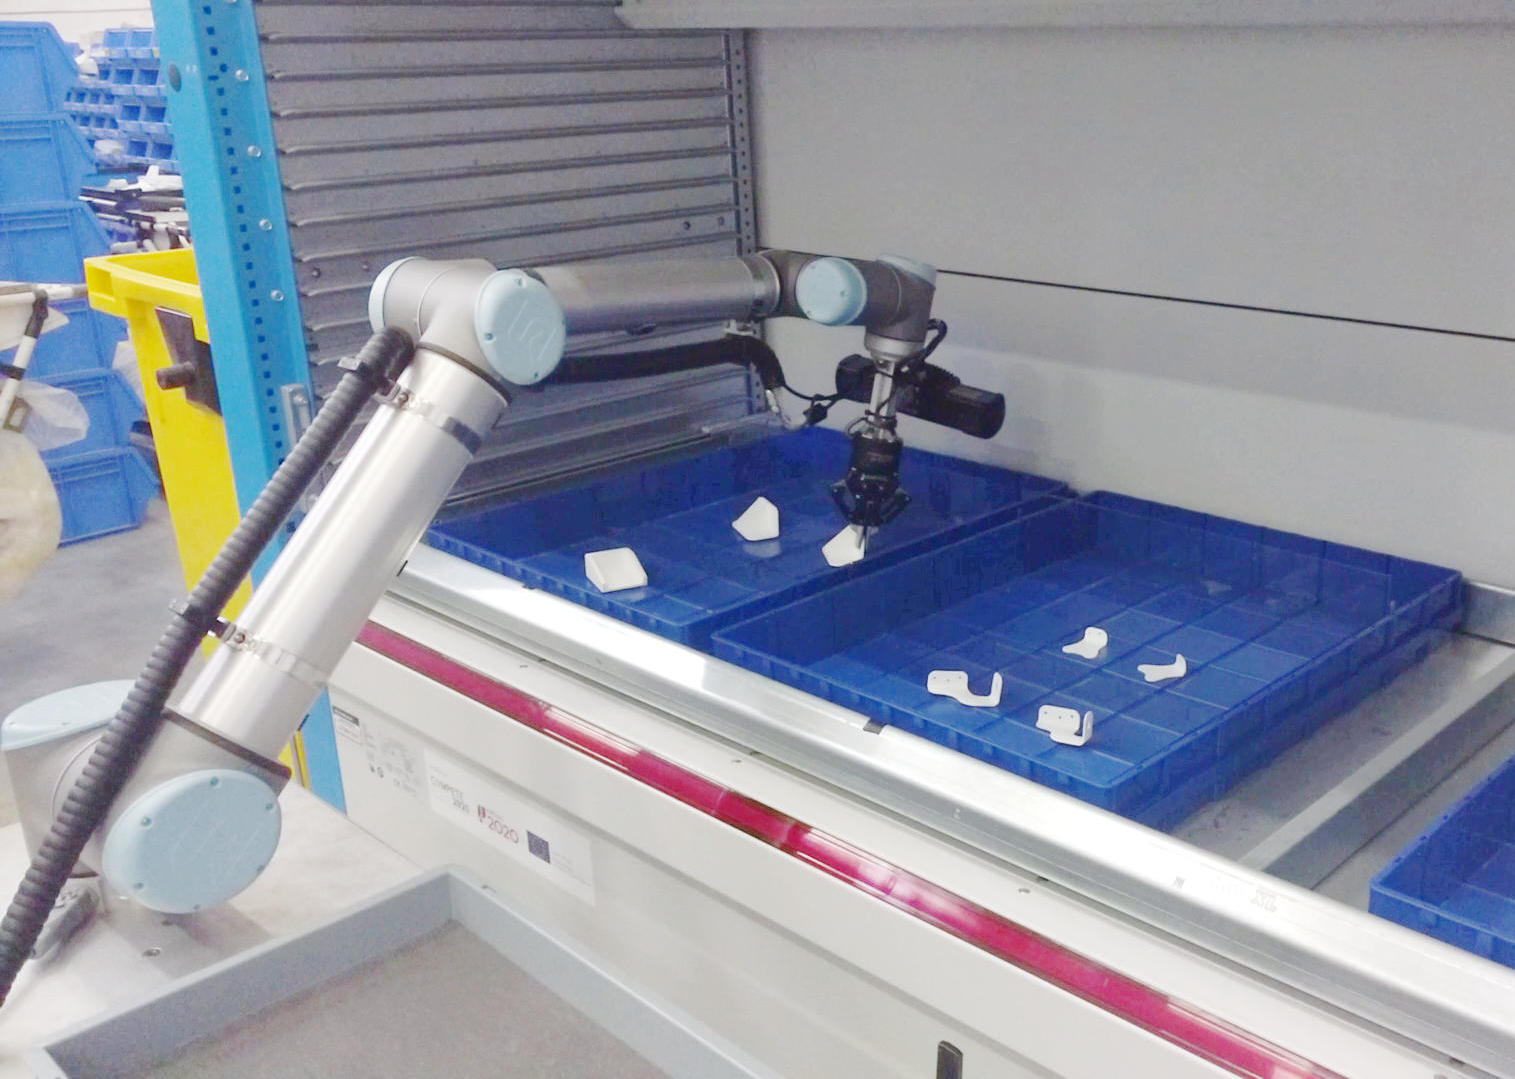
\includegraphics[height=.15\textheight]{Cap5/Figuras/picking_embraer/back-2}
	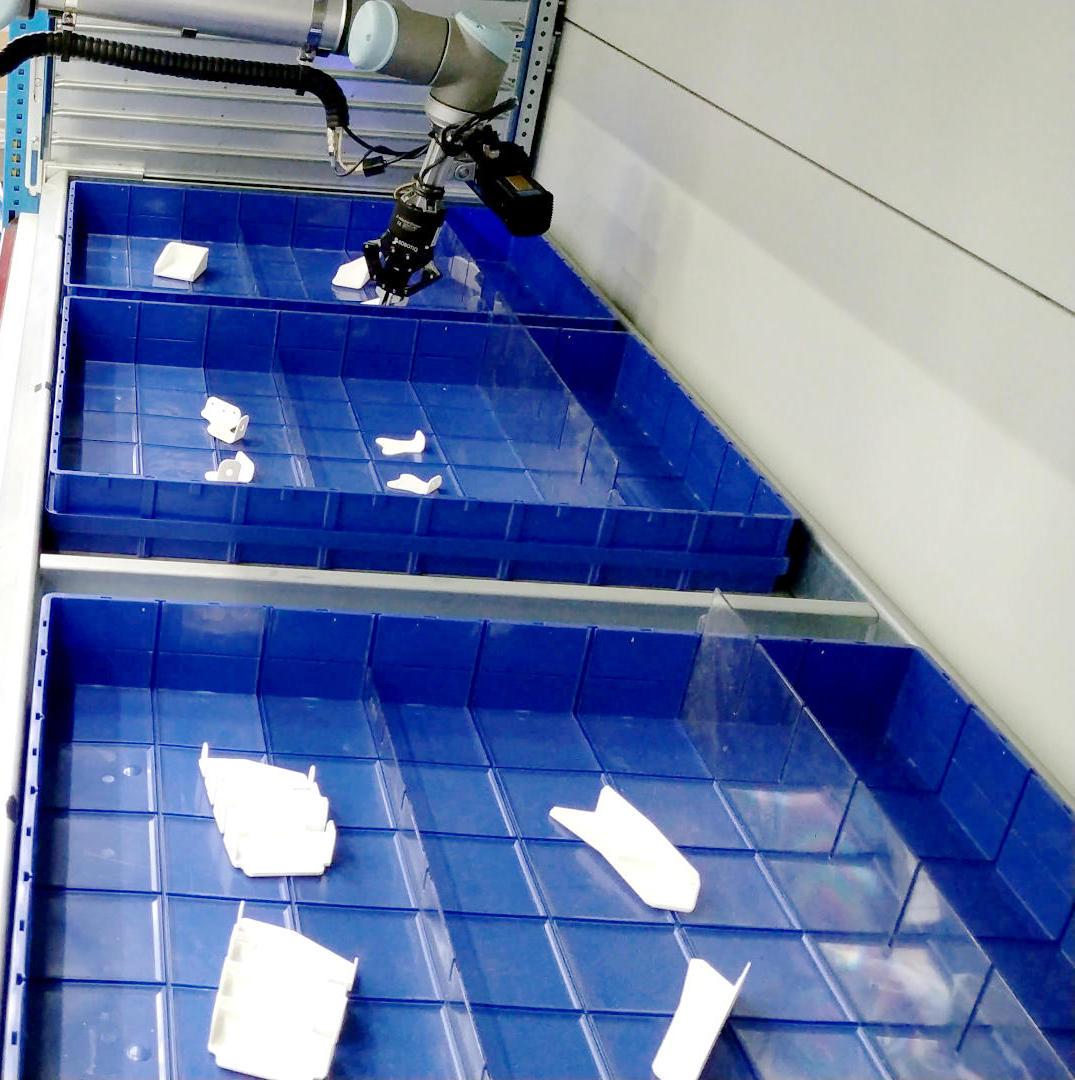
\includegraphics[height=.15\textheight]{Cap5/Figuras/picking_embraer/side-2}\\
	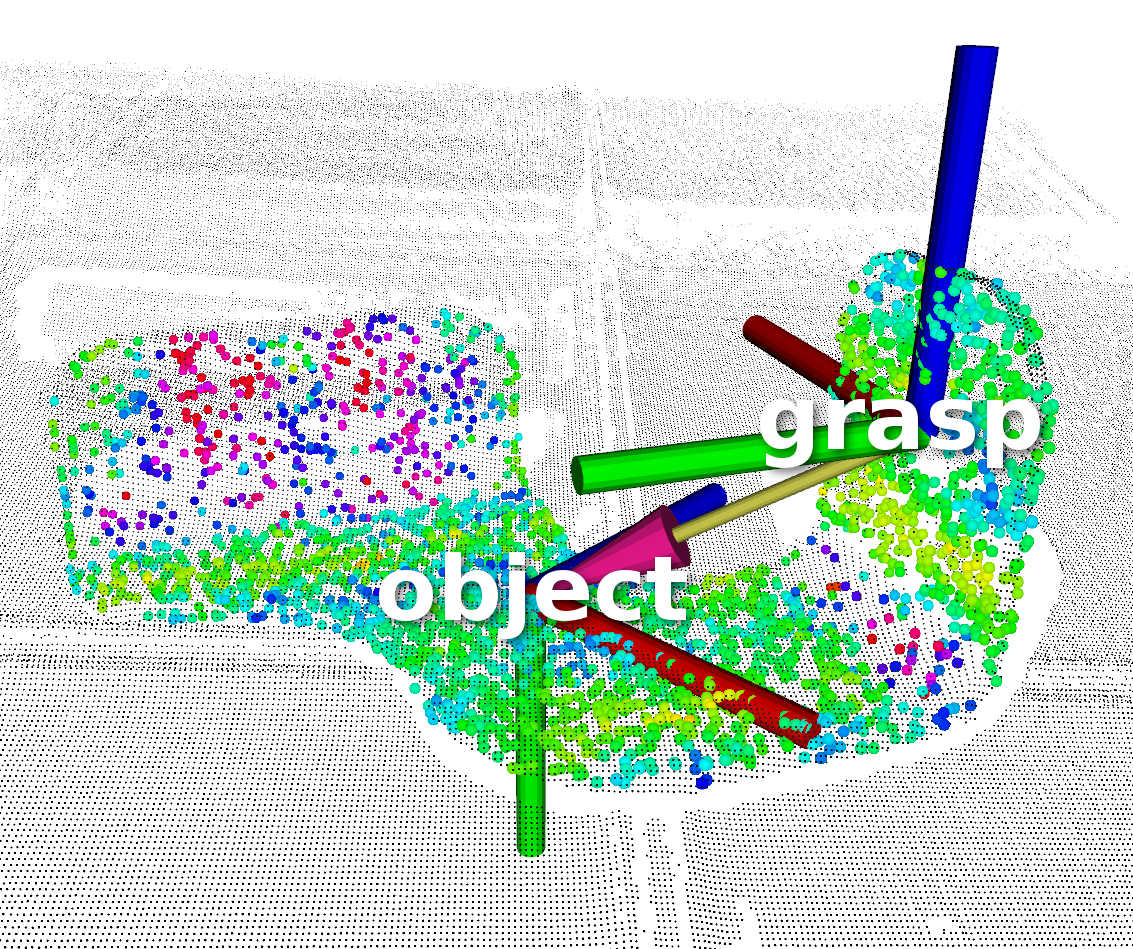
\includegraphics[height=.15\textheight]{Cap5/Figuras/picking_embraer/perception-3}
	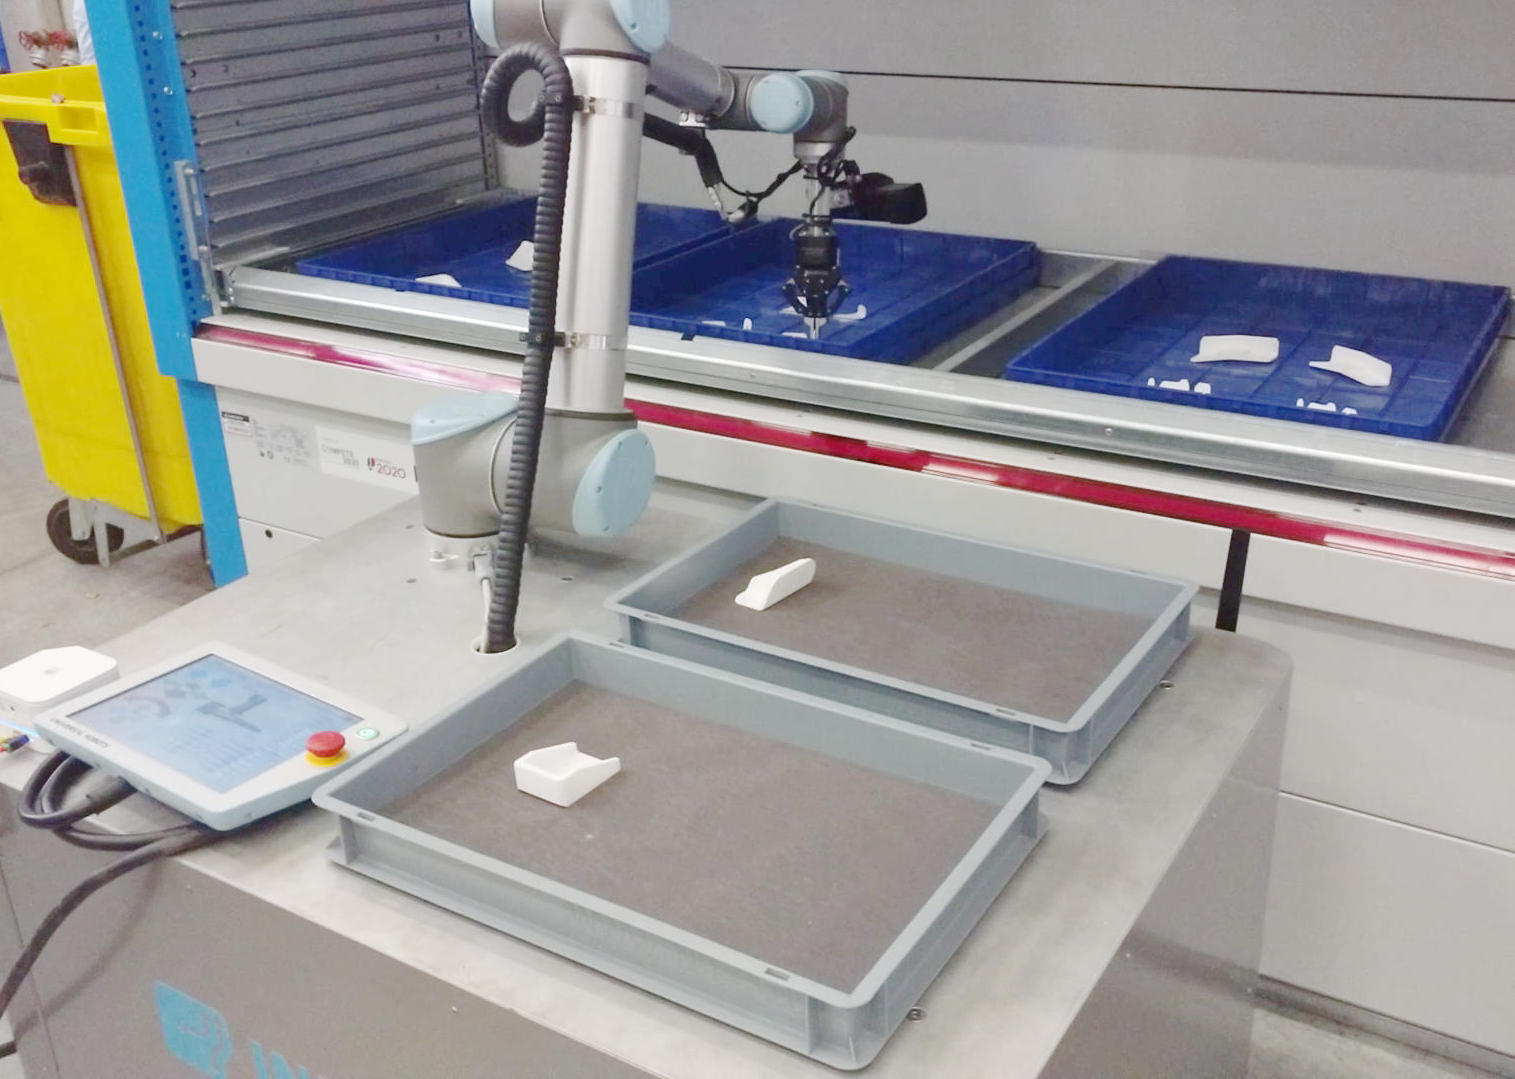
\includegraphics[height=.15\textheight]{Cap5/Figuras/picking_embraer/back-3}
	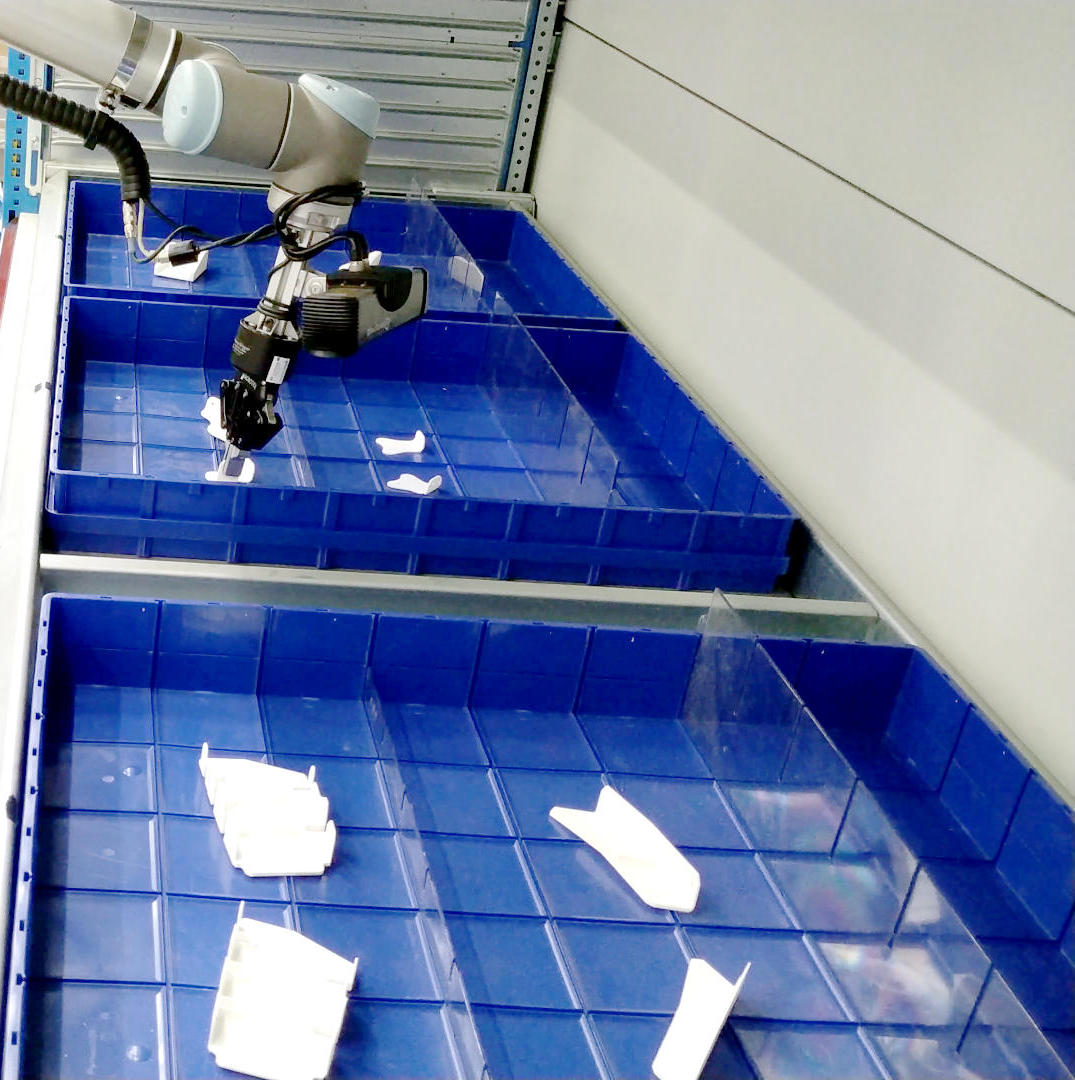
\includegraphics[height=.15\textheight]{Cap5/Figuras/picking_embraer/side-3}\\
	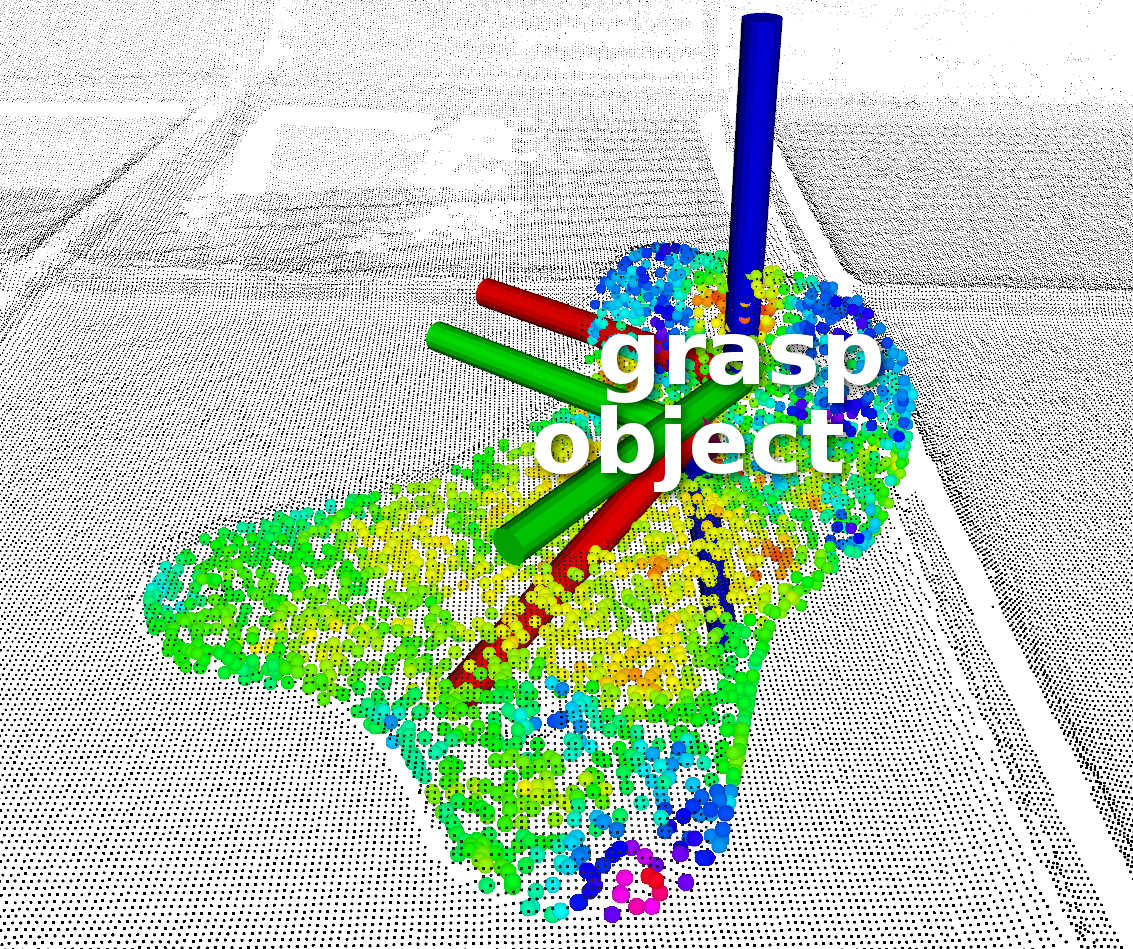
\includegraphics[height=.15\textheight]{Cap5/Figuras/picking_embraer/perception-4}
	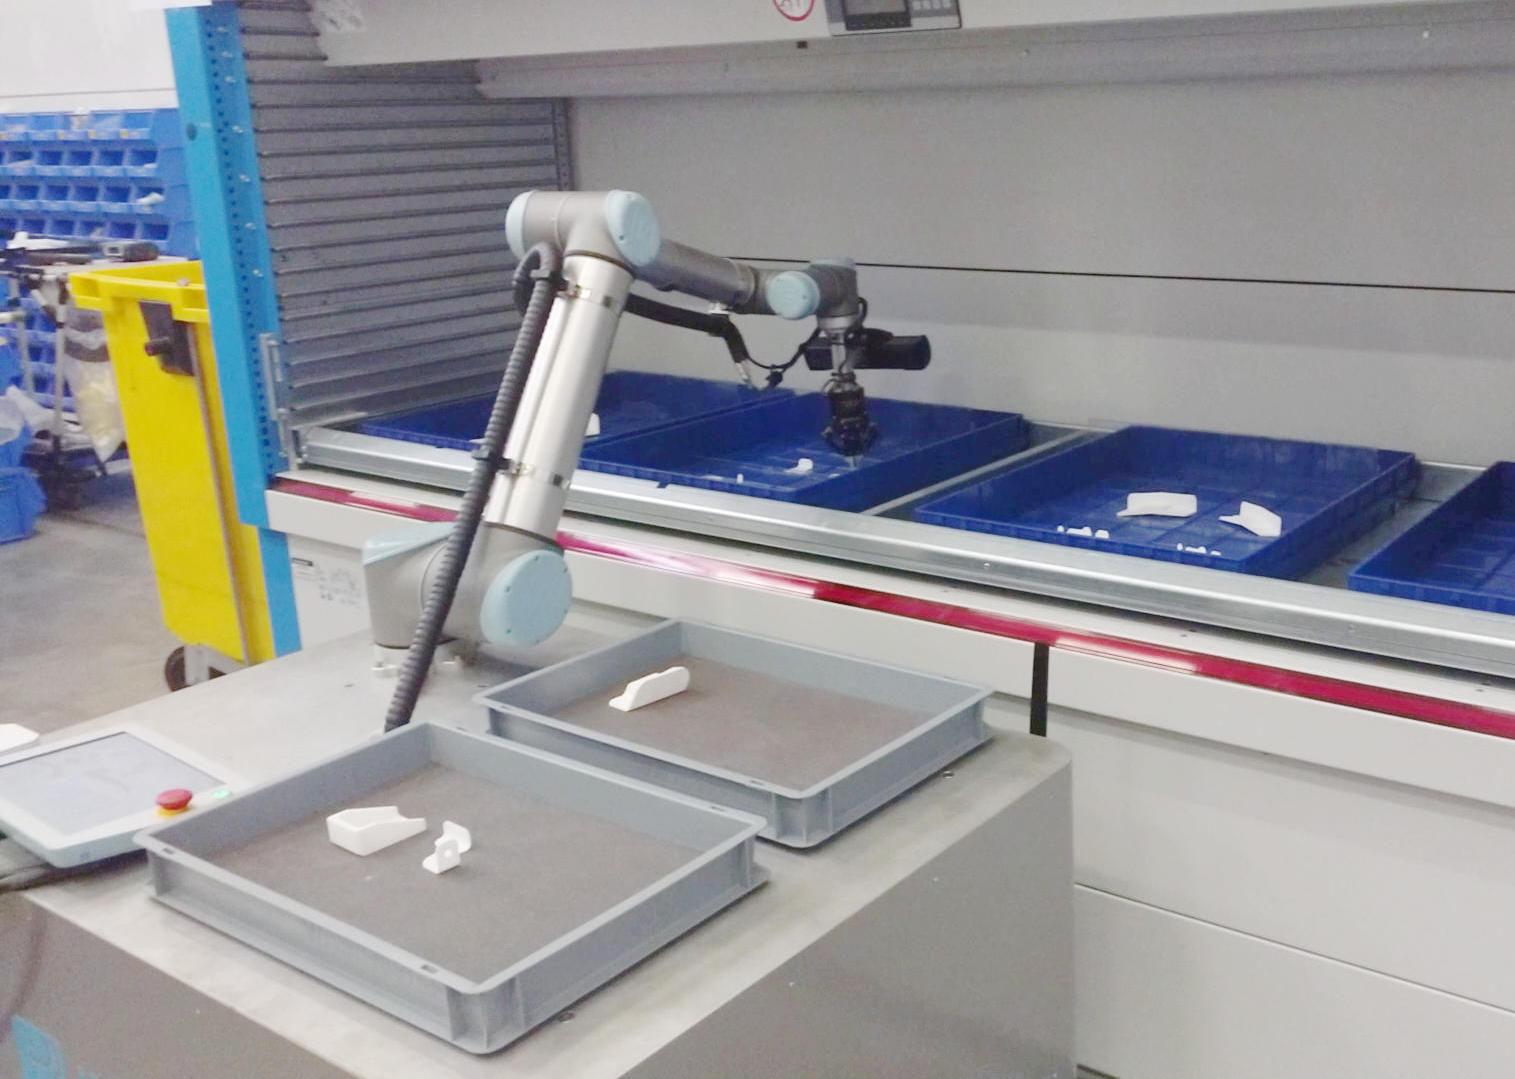
\includegraphics[height=.15\textheight]{Cap5/Figuras/picking_embraer/back-4}
	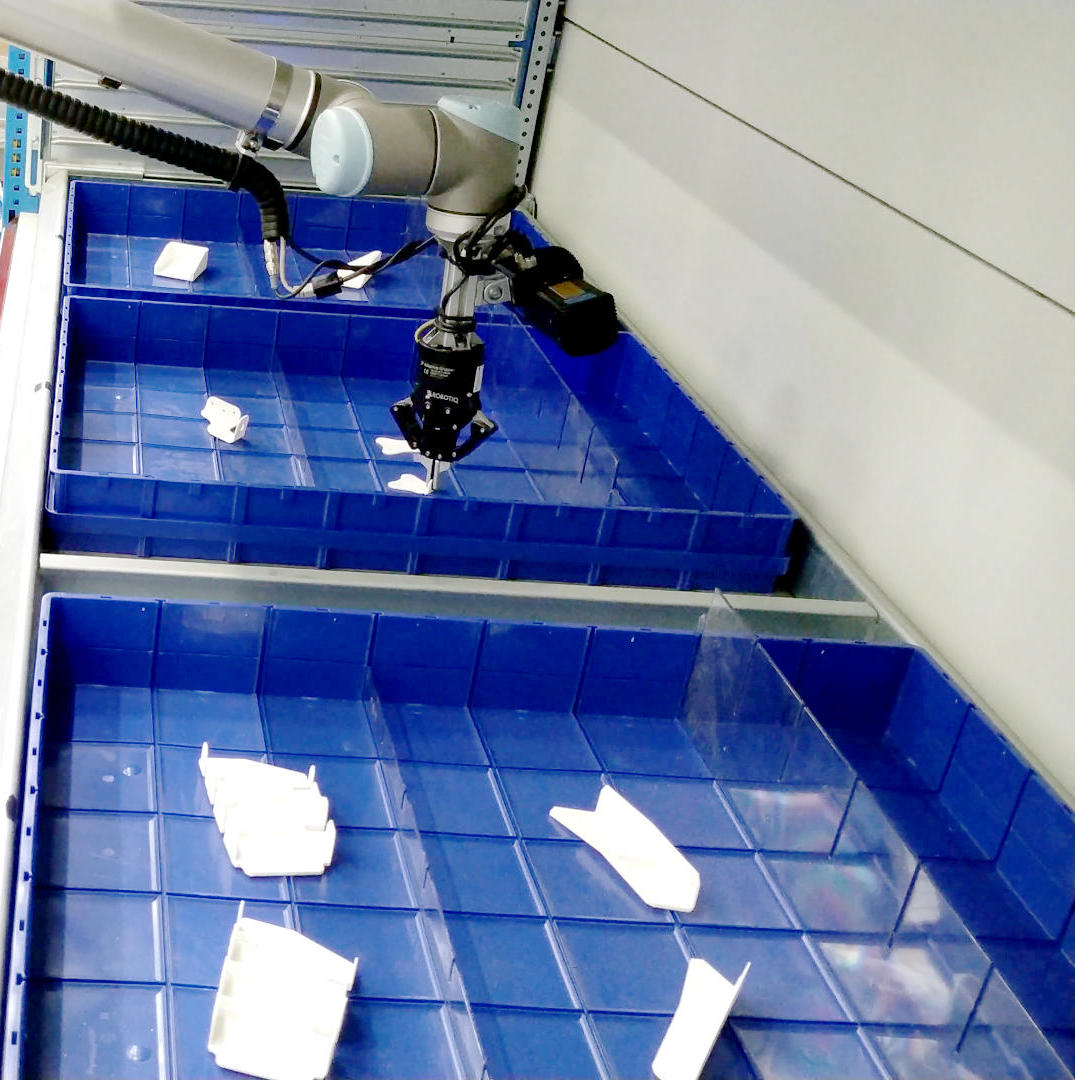
\includegraphics[height=.15\textheight]{Cap5/Figuras/picking_embraer/side-4}\\
	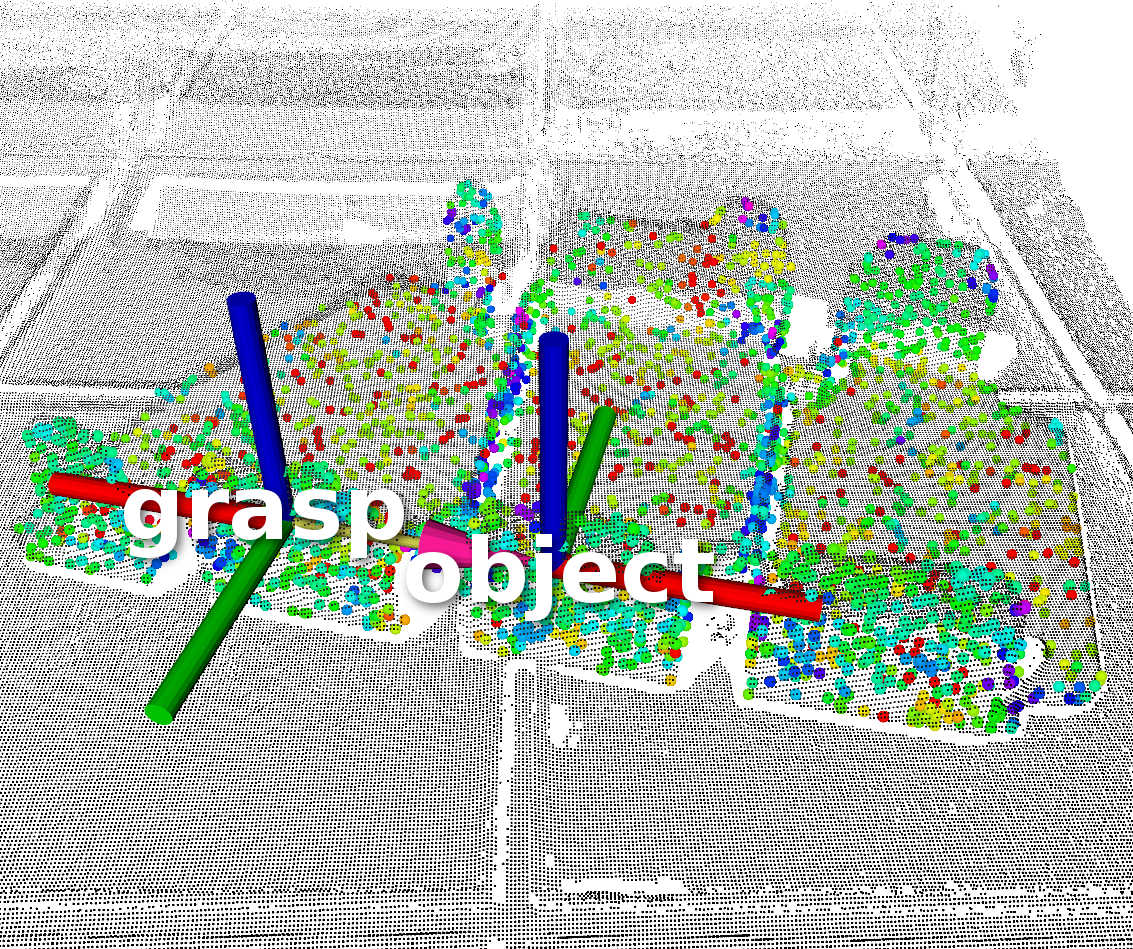
\includegraphics[height=.15\textheight]{Cap5/Figuras/picking_embraer/perception-5}
	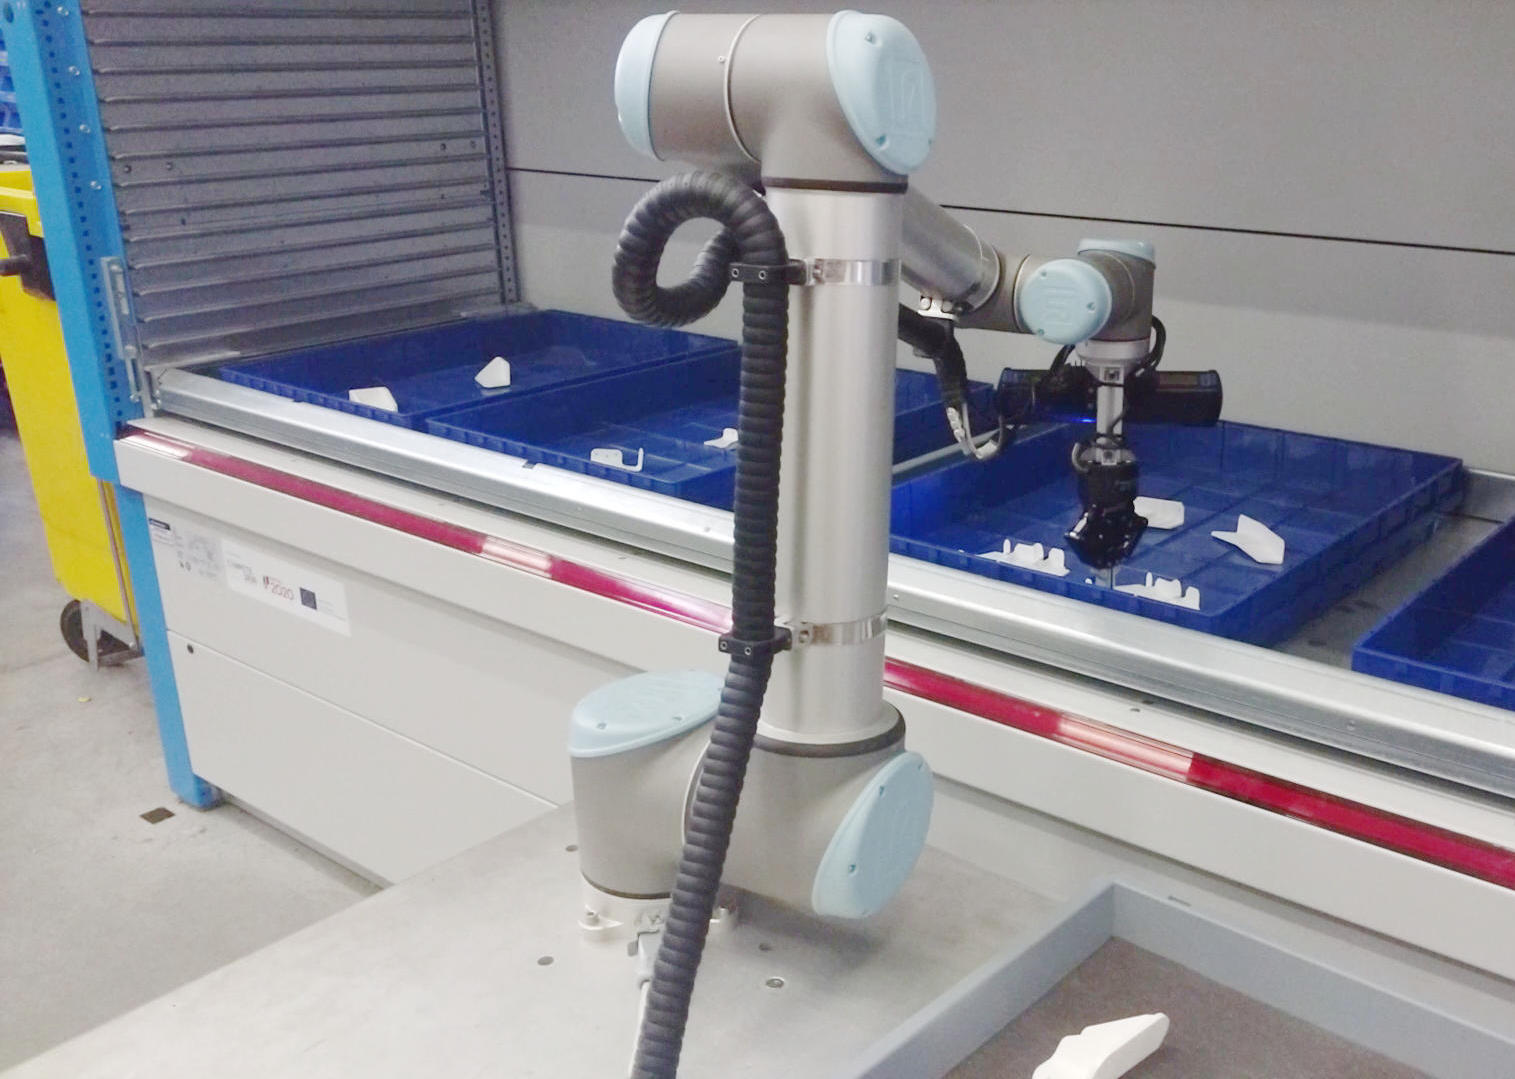
\includegraphics[height=.15\textheight]{Cap5/Figuras/picking_embraer/back-5}
	\includegraphics[height=.15\textheight]{Cap5/Figuras/picking_embraer/side-5}\\
	\includegraphics[height=.15\textheight]{Cap5/Figuras/picking_embraer/perception-6}
	\includegraphics[height=.15\textheight]{Cap5/Figuras/picking_embraer/back-6}
	\includegraphics[height=.15\textheight]{Cap5/Figuras/picking_embraer/side-6}
	\end{tcolorbox}
	\caption{Experimental grasping results in Embraer shop floor.}
	\label{fig:embraer_result}
}
\end{figure}


%\cred{TODO: inserir esta parte na conclusão}
%A priori, the strategy to naval use case were the deployment of the pneumatic grippers HGPC16A~\cite{festo_2f} and the foam suction cup FM-SW 76x22 4x6 N10~\cite{schmalz_cup}. However, along the project development and the access %to the naval pieces the grippers usage become unfeasible given the hardware restrictions on the omnidirectional robot leading to a new gripper hardware strategy, using the RobotiQ 2F-140. This shortcoming highlights the modularity %capability of the proposed pipeline, which in structured was not affected but only new configuration is defined to supply the new exigencies.


%\section{Mimic Grasping Evaluation}
\section{Mimic Grasping Evaluation}
\label{cap5:mimic_grasping_evaluation}

Since the ``Grasping Synthesis'' (``GraspIt!'' and ``Post-processors'') and the ``Grasping Selection'' were validated, tests regarding the ``Mimic Grasping Module''  were conducted at iiLab laboratory in INESCTEC facilities. It is used the use case \ac{OR} and 6DMimic to conduct a precision analysis of the proposal. Namely,  \ac{OR} is responsible to detect the object and the 6DMimic the tool pose, see Figure~\ref{fig:mimic_grapsing_procedure}.  The proposed GUI (Section~\ref{cap4:modular_grasping_architecture:sec:grasping_synthesis:subsec:mimic_grasping:subsubsec:gui}) allows graphical grasping feedback besides being responsible to load the ``Mimic Grasping API'', the configuration setup and the developed plugins. A detailed description of the proposal is discussed in Section~\ref{cap4:modular_grasping_architecture:sec:grasping_synthesis:subsec:mimic_grasping}, 


 \begin{figure}[h!]
 \resizebox{0.80\textwidth}{!}{%
 \begin{tcolorbox}
      \centering
      \begin{subfigure}[c]{.8\textwidth}
          \centering
          \includegraphics[trim={0cm 3.5cm 0cm 0cm},clip,width=1\linewidth,angle=0]{Cap4/Figuras/photo_use_case_overview_labeled.pdf}
          \caption{The use case setup.}
          \label{fig:mimic_grasping_test_idle}
      \end{subfigure}
      \hfill
      \begin{subfigure}[c]{.8\textwidth}
          \centering
          \includegraphics[width=1\textwidth]{Cap4/Figuras/photo_use_case_overview_flashing.pdf}
          \caption{The object pose estimation.}
          \label{fig:mimic_grasping_test_flashing}
      \end{subfigure}
      \hfill
      \begin{subfigure}[c]{.8\textwidth}
          \centering
          \includegraphics[width=1\textwidth]{Cap4/Figuras/photo_use_case_overview_demo.pdf}
          \caption{Tool handler pose acquisition, i.e. candidate generation.}
          \label{fig:mimic_grasping_test_demo}
      \end{subfigure}
     \end{tcolorbox}
     \caption{Precision analyses using the mimic grasping proposal.}
     \label{fig:mimic_grapsing_procedure}
   }%end of resize box      
 \end{figure}


The evaluation procedure consists of attaching a calibration probe to mimic grasping handler tool instead of a gripper. Afterwards, it is requested the handler tool poses at known-defined poses over the object. Figure~\ref{fig:mimic_grapsing_procedure} shows an example of this procedure. 

Two ground-truth pieces are designed to define the known poses, Figure~\ref{fig:groundtruth_pieces}. Both pieces are projected avoiding symmetries and looking for a better object recognition process. Each piece has small cavities along the axis with a defined pose w.r.t the object frame. The linear ground-truth piece's holes are spaced by 10 mm and the angular ground-truth piece's holes are spaced at 15 degrees. These holes work as a guide to the calibrated probe tool attached to the mimic grasping handler. Besides the pointed probe, applicable in the linear ground-truth piece, two other probes are designed (Figure~\ref{fig:probe_pointers}) intended for stable measurement acquisition over the angular ground-truth piece: the surface bracket and the yaw pointer. The pieces are printed using a Raise3D Pro Plus 3D printer with 0.28mm layer height~\cite{impressora3d}.


 \begin{figure}[h!]
 \resizebox{0.65\textwidth}{!}{%
 \begin{tcolorbox}
      \centering
      \begin{subfigure}[c]{.485\textwidth}
          \centering
          \includegraphics[trim={6cm 2cm 6cm 2cm},clip,width=1\linewidth,angle=0]{Cap5/Figuras/linear_gt2.pdf}
          \caption{Linear ground-truth piece.}
          \label{fig:linear_gt}
      \end{subfigure}
      \hfill
      \begin{subfigure}[c]{.485\textwidth}
          \centering
          \includegraphics[trim={6cm 2cm 6cm 2cm},clip,width=1\linewidth,angle=0]{Cap5/Figuras/angular_gt2.pdf}
          \caption{Angular ground-truth piece.}
          \label{fig:angular_gt}
      \end{subfigure}
     \end{tcolorbox}
     \caption{The designed ground-truth pieces.}
     \label{fig:groundtruth_pieces}
   }%end of resize box      
 \end{figure}
 
 
  \begin{figure}[h!]
 \resizebox{.75\textwidth}{!}{%
 \begin{tcolorbox}
      \centering
      \begin{subfigure}[c]{.30\textwidth}
          \centering
          \includegraphics[trim={4cm 0.5cm 3cm 5cm},clip,width=1\linewidth,angle=0]{Cap5/Figuras/ponta_prova_thin.pdf}
          \caption{Probe pointer.}
          \label{fig:probe_pointer}
      \end{subfigure}
      \hfill
      \begin{subfigure}[c]{.30\textwidth}
          \centering
          \includegraphics[trim={3cm 1cm 5cm 2cm},clip,width=1\linewidth,angle=0]{Cap5/Figuras/ponta_prova_surface.pdf}
          \caption{Surface bracket.}
          \label{fig:surface_bracket_probe_pointer}
      \end{subfigure}
      \hfill
      \begin{subfigure}[c]{.25\textwidth}
          \centering
          \includegraphics[trim={1cm 3cm 6cm 4cm},clip,width=1\linewidth,angle=0]{Cap5/Figuras/ponta_prova_yaw.pdf}
          \caption{Yaw pointer.}
          \label{fig:yaw_probe_pointer}
      \end{subfigure}
     \end{tcolorbox}
     \caption{The designed probes attached on tool handler.}
     \label{fig:probe_pointers}
   }%end of resize box      
 \end{figure}
 
 
It is expected that all measurements incorporate a residual offset and linear component due to calibration inconsistencies. Since this is a systematic error, results could be improved by predicting the error and adjusting it. Therefore, ten acquisitions are performed for each pose component using the ground-truth pieces. The error is estimated by manually placing the probe tool on a cavity, requesting grasping capture and verifying the difference between the ground-truth position/orientation and the acquisition pose. This analysis procedure is realised for each axis simplifying the manual analyses procedure. Acquisition examples are presented in Figure~\ref{fig:precision_linear_asses} and Figure~\ref{fig:precision_angular_asses} for linear and angular ground-truth pieces, respectively.

 \begin{figure}[h!]
 \resizebox{.6\textwidth}{!}{%
 \begin{tcolorbox}
      \centering
      \begin{subfigure}[c]{1\textwidth}
          \centering
          \includegraphics[trim={0cm 0cm 0cm 0cm},clip,width=1\linewidth,angle=0]{Cap5/Figuras/demo_x_axis.pdf}
          \caption{X-axis.}
          \label{fig:x-axis-asses}
      \end{subfigure}
      \hfill
      \begin{subfigure}[c]{1\textwidth}
          \centering
          \includegraphics[trim={0cm 0cm 0cm 0cm},clip,width=1\linewidth,angle=0]{Cap5/Figuras/demo_y_axis.pdf}
          \caption{Y-axis.}
          \label{fig:y-axis-asses}
      \end{subfigure}
      \hfill
      \begin{subfigure}[c]{1\textwidth}
          \centering
          \includegraphics[trim={0cm 0cm 0cm 0cm},clip,width=1\linewidth,angle=0]{Cap5/Figuras/demo_z_axis.pdf}
          \caption{Z-axis.}
          \label{fig:z-axis-asses}
     \end{subfigure}
     \end{tcolorbox}
     \caption{Precision assessment procedure using linear ground-truth piece.}
     \label{fig:precision_linear_asses}
   }%end of resize box      
 \end{figure}
 
 \begin{figure}[h!]
 \resizebox{.6\textwidth}{!}{%
 \begin{tcolorbox}
      \centering
      \begin{subfigure}[c]{1\textwidth}
          \centering
          \includegraphics[trim={0cm 0cm 0cm 0cm},clip,width=1\linewidth,angle=0]{Cap5/Figuras/demo_roll_axis.pdf}
          \caption{Roll.}
          \label{fig:roll-axis-asses}
      \end{subfigure}
      \hfill
      \begin{subfigure}[c]{1\textwidth}
          \centering
          \includegraphics[trim={0cm 0cm 0cm 0cm},clip,width=1\linewidth,angle=0]{Cap5/Figuras/demo_pitch_axis.pdf}
          \caption{Pitch.}
          \label{fig:pitch-axis-asses}
      \end{subfigure}
      \hfill
      \begin{subfigure}[c]{1\textwidth}
          \centering
          \includegraphics[trim={0cm 0cm 0cm 0cm},clip,width=1\linewidth,angle=0]{Cap5/Figuras/demo_yaw_axis.pdf}
          \caption{Yaw.}
          \label{fig:yaw-axis-asses}
     \end{subfigure}
     \end{tcolorbox}
     \caption{Precision assessment procedure using angular ground-truth piece.}
     \label{fig:precision_angular_asses}
   }%end of resize box      
 \end{figure}

The mean acquisition error for each ground-truth component pose in association with the predicted error curve is presented in Figure~\ref{fig:mimic_grasping_prediction_error_curve}.
Linear regression  with a confidence interval of 0.95 is applied to build the prediction curve. Therefore, each component prediction value is defined by a linear equation~\ref{eq:linear_eq}.

\begin{figure}[h!]
\resizebox{1\textwidth}{!}{%
\begin{tcolorbox}
     \centering
     \begin{subfigure}[c]{.485\textwidth}
         \centering
         \includegraphics[width=1\textwidth]{Cap5/Figuras/x_correction_asses.pdf}
         %\caption{}
         %\label{fig:x_linear_regression}
     \end{subfigure}
     \hfill
     \begin{subfigure}[c]{.485\textwidth}
         \centering
         \includegraphics[width=1\textwidth]{Cap5/Figuras/y_correction_asses.pdf}
         %\caption{}
         %\label{fig:y_linear_regression}
     \end{subfigure}
     \hfill
     \begin{subfigure}[c]{.485\textwidth}
         \centering
         \includegraphics[width=1\textwidth]{Cap5/Figuras/z_correction_asses.pdf}
         %\caption{Pure force closure.}
         %\label{fig:z_linear_regression}
     \end{subfigure}
     \begin{subfigure}[c]{.485\textwidth}
         \centering
         \includegraphics[width=1\textwidth]{Cap5/Figuras/roll_correction_asses.pdf}
         %\caption{}
         %\label{fig:roll_linear_regression}
     \end{subfigure}
     \hfill
     \begin{subfigure}[c]{.485\textwidth}
         \centering
         \includegraphics[width=1\textwidth]{Cap5/Figuras/pitch_correction_asses.pdf}
         %\caption{}
         %\label{fig:pitch_linear_regression}
     \end{subfigure}
     \hfill
     \begin{subfigure}[c]{.485\textwidth}
         \centering
         \includegraphics[width=1\textwidth]{Cap5/Figuras/yaw_correction_asses.pdf}
         %\caption{}
         %\label{fig:yaw_linear_regression}
     \end{subfigure}
    \end{tcolorbox}
    \caption{Predicted correction curve for all components of a candidate.}
    \label{fig:mimic_grasping_prediction_error_curve}
  }%end of resize box      
\end{figure}

\begin{equation}
   \Delta e = a\cdot x + b 
   \label{eq:linear_eq}
\end{equation}

where $\Delta e$ is the predicted error; $x$ the candidate component measurement; $a$ the line slope and $b$ the linear y-intercept parameters. Table~\ref{tab:ab_table} shows the estimated coefficients $a$ and $b$ which is applied into Mimic Grasping Pipeline by filling the error compensation file (Section~\ref{cap4:modular_grasping_architecture:sec:grasping_synthesis:subsec:graspit:subsubsec:sann}).

\begin{table}[h!]
\resizebox{.55\textwidth}{!}{%
\begin{tcolorbox}
\centering
\caption{Prediction errors linear parameters.}
\label{tab:ab_table}
\resizebox{\textwidth}{!}{%
\begin{tabular}{@{}ccc@{}}
\toprule
\textbf{Candidate's Component} & \textbf{Slope} & \textbf{Y-Intercept} \\ \midrule
X-Axis                         & -0.00296       & 0.00274              \\
Y-Axis                         & -0.00452       & 0.00378              \\
Z-Axis                         & -0.00396       & 0.00891              \\
Roll                           & -0.0373        & 2.10191              \\
Pitch                          & -0.03013       & 2.77801              \\
Yaw                            & -0.02383       & -1.85640             \\ \bottomrule
\end{tabular}%
}
\end{tcolorbox}
}
\end{table}


Along with the error prediction estimated for the given use case, new acquisitions are executed using both ground-truth pieces. A total of 816 grasping acquisitions were performed. The visual \ac{GUI} feedback (Section~\ref{cap4:modular_grasping_architecture:sec:grasping_synthesis:subsec:mimic_grasping:subsubsec:gui}), which update in demonstration-time, allows to identify  a total of 37 outliers that were deleted by the tool handler firmware ``Cancelling'' state (Section~\ref{cap4:modular_grasping_architecture:sec:grasping_synthesis:subsec:mimic_grasping:subsubsec:firmware}). Therefore the pipeline was able to generate feasible grasping poses at a \ac{GPSR} of 95.47\%. These outliers candidates are typically generated when the handler tool's luminous marker is out of 6D Mimic camera's workspace or if any critical occlusion is created. 


The final precision result assessment is defined by the curves of Figure~\ref{fig:mimic_grapsing_final_error}. In these plots it is possible to verify that the strategy to remove the systematic error improves the result, e.g. considering the absolute average error of all measurements, the x-axis, y-axis and z-axis errors improve in 2.5mm, 2.34mm and 8.63mm. Regarding the roll, pitch, and yaw errors the improvements are of 2.63$^o$, 1.83$^o$ and 3.82$^o$, respectively. It is important to note that, since the 6D Mimic is a stereoscopic system, the acquisitions transversal to the cameras' baseline incorporate a larger error than the ones that are in the image plane. Therefore, in the present use case,  the linear ground-truth piece configuration includes a larger and a small transversal stereoscopic error along the y-axis and x-axis, respectively, which define the larger error detected in plots of these components concerning the z-axis that is completely in the image plane. The high error over the z-axis The angular assessments variance is due to the fact the process is manually performed, thus inconsistencies occur based on human movements. However, these results variances result in permissive error values regarding grasping objects.

\begin{figure}[h!]
\resizebox{1\textwidth}{!}{%
\begin{tcolorbox}
     \centering
     \begin{subfigure}[c]{.485\textwidth}
         \centering
         \includegraphics[width=1\textwidth]{Cap5/Figuras/x.pdf}
         %\caption{}
         %\label{fig:x_test}
     \end{subfigure}
     \hfill
     \begin{subfigure}[c]{.485\textwidth}
         \centering
         \includegraphics[width=1\textwidth]{Cap5/Figuras/y.pdf}
         %\caption{}
         %\label{fig:y_test}
     \end{subfigure}
     \hfill
     \begin{subfigure}[c]{.485\textwidth}
         \centering
         \includegraphics[width=1\textwidth]{Cap5/Figuras/z.pdf}
         %\caption{}
         %\label{fig:z_test}
     \end{subfigure}
    %\caption{Linear components error of a candidate.}
    %\label{fig:mimic_grapsing_linear_error}
     \begin{subfigure}[c]{.485\textwidth}
         \centering
         \includegraphics[width=1\textwidth]{Cap5/Figuras/roll.pdf}
         %\caption{}
         %\label{fig:roll_test}
     \end{subfigure}
     \hfill
     \begin{subfigure}[c]{.485\textwidth}
         \centering
         \includegraphics[width=1\textwidth]{Cap5/Figuras/pitch.pdf}
         %\caption{}
         %\label{fig:pitch_test}
     \end{subfigure}
     \hfill
     \begin{subfigure}[c]{.485\textwidth}
         \centering
         \includegraphics[width=1\textwidth]{Cap5/Figuras/yaw.pdf}
         %\caption{}
         %\label{fig:yaw_test}
     \end{subfigure}
    \end{tcolorbox}
    \caption{Components error of a candidate.}
    \label{fig:mimic_grapsing_final_error}
  }%end of resize box      
\end{figure}


With the system properly configured and assessed, grasping demonstrations are performed using the mimic grasping system discussed in this section. The Figure~\ref{fig:demos_mimic_grasping} shows grasping examples executed by IRB2600 robot using the grippers HGPC16A~\cite{festo_2f} and the foam suction cup FM-SW 76x22 4x6 N10~\cite{schmalz_cup} (Figure~\ref{fig:mimic_grippers_supported}) which are mimic of a human movement.


%\begin{figure}[h!]
%\resizebox{1\textwidth}{!}{%
%\begin{tcolorbox}
%\centerline{\includegraphics[trim={0cm 6cm 8cm 1cm},clip,width=.75\linewidth,angle=0]{Cap5/Figuras/demo_01.pdf}}
%\end{tcolorbox}
%\caption{Demonstration process using the Foam suction cup gripper.}
%\label{fig:demo_01}
%}%end resize box
%\end{figure}


\begin{figure}[h!]
\resizebox{1\textwidth}{!}{%
\begin{tcolorbox}
     \centering
     \begin{subfigure}[c]{.495\textwidth}
         \centering
         \includegraphics[trim={0cm 6cm 8cm 0cm},clip,width=1\linewidth,angle=0]{Cap5/Figuras/demo_02.pdf}
         \caption{Two-finger grasping with HGPC16A.}
         \label{fig:demo_02}
     \end{subfigure}
     %\hfill
     \begin{subfigure}[c]{.495\textwidth}
         \centering
         \includegraphics[trim={0cm 6cm 8cm 0cm},clip,width=1\linewidth,angle=0]{Cap5/Figuras/demo_01.pdf}
         \caption{Suction grasping with FM-SW.}
         \label{fig:demo_01}
     \end{subfigure}
    \end{tcolorbox}
    \caption{Mimic grasping candidate building using the linear ground truth object and two different grippers. First the human demonstration, following by the Mimic Grasping GUI representation and the robot grasping movement.}
    \label{fig:demos_mimic_grasping}
  }%end of resize box      
\end{figure}




